\documentclass[12pt,spanish,fleqn,openany,letterpaper,pagesize]{scrbook}

%\usepackage[ansinew]{inputenc}
\usepackage[spanish]{babel}
\usepackage[utf8]{inputenc}
\usepackage[T1]{fontenc}
\usepackage{fancyhdr}
\usepackage{epsfig}
\usepackage{epic}
\usepackage{url}
\usepackage{sectsty}
\usepackage{lipsum}
\usepackage{enumitem}
\usepackage[T1]{fontenc}
\usepackage{pslatex}
\usepackage{gensymb}
% \usepackage{hyperref}

\usepackage{eepic}
\usepackage{amsmath}
\usepackage{nccmath}
\usepackage{threeparttable}
\usepackage{amscd}
\usepackage{here}
\usepackage{graphicx}
\usepackage{lscape}
\usepackage{tabularx}
\usepackage{subfigure}
\usepackage{longtable}
\usepackage{amssymb}
\usepackage{rotating} %Para rotar texto, objetos y tablas seite. No se ve en DVI solo en PS. Seite 328 Hundebuch                        %se usa junto con \rotate, \sidewidestable                        ....
\usepackage{listings}
\usepackage{color}

\definecolor{dkgreen}{rgb}{0,0.6,0}
\definecolor{gray}{rgb}{0.5,0.5,0.5}
\definecolor{mauve}{rgb}{0.58,0,0.82}

\lstset{frame=tb,
  language=Java,
  aboveskip=3mm,
  belowskip=3mm,
  showstringspaces=false,
  columns=flexible,
  basicstyle={\small\ttfamily},
  numbers=none,
  numberstyle=\tiny\color{gray},
  keywordstyle=\color{blue},
  commentstyle=\color{dkgreen},
  stringstyle=\color{mauve},
  breaklines=true,
  breakatwhitespace=true,
  tabsize=3
}
\lstset{extendedchars=\true}
\lstset{literate=
  {á}{{\'a}}1 {é}{{\'e}}1 {í}{{\'i}}1 {ó}{{\'o}}1 {ú}{{\'u}}1
  {Á}{{\'A}}1 {É}{{\'E}}1 {Í}{{\'I}}1 {Ó}{{\'O}}1 {Ú}{{\'U}}1
  {à}{{\`a}}1 {è}{{\`e}}1 {ì}{{\`i}}1 {ò}{{\`o}}1 {ù}{{\`u}}1
  {À}{{\`A}}1 {È}{{\'E}}1 {Ì}{{\`I}}1 {Ò}{{\`O}}1 {Ù}{{\`U}}1
  {ä}{{\"a}}1 {ë}{{\"e}}1 {ï}{{\"i}}1 {ö}{{\"o}}1 {ü}{{\"u}}1
  {Ä}{{\"A}}1 {Ë}{{\"E}}1 {Ï}{{\"I}}1 {Ö}{{\"O}}1 {Ü}{{\"U}}1
  {â}{{\^a}}1 {ê}{{\^e}}1 {î}{{\^i}}1 {ô}{{\^o}}1 {û}{{\^u}}1
  {Â}{{\^A}}1 {Ê}{{\^E}}1 {Î}{{\^I}}1 {Ô}{{\^O}}1 {Û}{{\^U}}1
  {Ã}{{\~A}}1 {ã}{{\~a}}1 {Õ}{{\~O}}1 {õ}{{\~o}}1
  {œ}{{\oe}}1 {Œ}{{\OE}}1 {æ}{{\ae}}1 {Æ}{{\AE}}1 {ß}{{\ss}}1
  {ű}{{\H{u}}}1 {Ű}{{\H{U}}}1 {ő}{{\H{o}}}1 {Ő}{{\H{O}}}1
  {ç}{{\c c}}1 {Ç}{{\c C}}1 {ø}{{\o}}1 {å}{{\r a}}1 {Å}{{\r A}}1
  {€}{{\euro}}1 {£}{{\pounds}}1 {«}{{\guillemotleft}}1
  {»}{{\guillemotright}}1 {ñ}{{\~n}}1 {Ñ}{{\~N}}1 {¿}{{?`}}1
}

\renewcommand{\theequation}{\thechapter-\arabic{equation}}
\renewcommand{\thefigure}{\textbf{\thechapter-\arabic{figure}}}
\renewcommand{\thetable}{\textbf{\thechapter-\arabic{table}}}
\pagestyle{fancyplain}%\addtolength{\headwidth}{\marginparwidth}
\oddsidemargin0.5cm \topmargin-1cm \evensidemargin-0.5cm
\renewcommand{\chaptermark}[1]{\markboth{\thechapter\; #1}{}}
\renewcommand{\sectionmark}[1]{\markright{\thesection\; #1}}
%\lhead[\fancyplain{}{\thepage}]{\fancyplain{}{\rightmark}}
%\rhead[\fancyplain{}{\leftmark}]{\fancyplain{}{\thepage}}

\chapterfont{\centering}
\addtolength{\headwidth}{-0.5cm}
\unitlength1mm %Define la unidad LE para Figuras
\mathindent0cm %Define la distancia de las formulas al texto,  fleqn las descentra
\marginparwidth0cm
\parindent0cm %Define la distancia de la primera linea de un parrafo a la margen

\usepackage[top=3cm,bottom=3cm,left=4cm,right=2cm]{geometry} 
\fancyfoot[CE,CO]{\thepage}
\textheight21.3cm
%Para tablas,  redefine el backschlash en tablas donde se define la posici\'{o}n del texto en las
%casillas (con \centering \raggedright o \raggedleft)
\newcommand{\PreserveBackslash}[1]{\let\temp=\\#1\let\\=\temp}
\let\PBS=\PreserveBackslash

%Espacio entre lineas
\renewcommand{\baselinestretch}{1.1}

%Neuer Befehl f\"{u}r die Tabelle Eigenschaften der Aktivkohlen
\newcommand{\arr}[1]{\raisebox{1.5ex}[0cm][0cm]{#1}}

%Neue Kommandos
\usepackage{Befehle}


%Trennungsliste
\hyphenation {Reaktor-ab-me-ssun-gen Gas-zu-sa-mmen-set-zung
Raum-gesch-win-dig-keit Durch-fluss Stick-stoff-gemisch
Ad-sorp-tions-tem-pe-ra-tur Klein-schmidt
Kohlen-stoff-Mole-kular-siebe Py-rolysat-aus-beu-te
Trans-port-vor-gan-ge}

\begin{document}
\pagenumbering{roman}
%CUBIERTA
\begin{center}
\thispagestyle{empty} \vspace*{0cm} \huge\textbf{
Diseño e Implementaci\'{o}n de un Medidor de Energ\'{i}a Trif\'{a}sica para Sistemas El\'{e}ctricos no Lineales. }\\[6.0cm]
\Large\textbf{German Andres Sanchez Motta\\Kevin Fabian Carrillo Carrillo}\\[6.0cm]
\small Universidad Santo Tomas\\
Facultad de Ingenier\'{i}a Electr\'{o}nica\\
Bogot\'{a}, Colombia\\
2018\\
\end{center}

\newpage{\pagestyle{empty}\clearpage}

%PORTADA
\newpage
\begin{center}
\thispagestyle{empty} \vspace*{0cm} \huge\textbf{
Diseño e Implementaci\'{o}n de un Medidor de Energ\'{i}a Trif\'{a}sica para Sistemas El\'{e}ctricos no Lineales. }\\[2.5cm]
\Large\textbf{German Andres Sanchez Motta\\Kevin Fabian Carrillo Carrillo}\\[2.5cm]
\small Monograf\'{i}a de proyecto de grado para optar al
t\'{\i}tulo de:\\
\textbf{Ingeniero Electr\'{o}nico }\\[2.5cm]

Director:\\
Ing. Edwin Francisco Forero Garcia, M.Sc.\\[3.7cm]




Universidad Santo Tomas\\
Facultad de Ingenier\'{i}a Electr\'{o}nica \\
Bogot\'{a}, Colombia\\
2018\\
\end{center}


%DEDICATORIA
\newpage{\clearpage}
\thispagestyle{empty} \textbf{}\normalsize
\\\\\\%
\textbf{\LARGE Dedicatoria}\\[4.0cm]
\setcounter{page}{3}
\addcontentsline{toc}{chapter}{\numberline{}Dedicatoria}\\\\

\begin{flushright}
\begin{minipage}{8cm}
    \noindent
        \small
		Principalmente a Dios y después a nuestros padres, quienes fueron de gran ayuda y confianza incondicional en esta trayectoria de formación personal y profesional.  \\[4.0cm]\\
        
\end{minipage}
\end{flushright}


%AGRADECIMIENTOS
\newpage{\clearpage}
\thispagestyle{empty} \textbf{}\normalsize
\\\\\\%
\textbf{\LARGE Agradecimientos}
\setcounter{page}{5}
\addcontentsline{toc}{chapter}{\numberline{}Agradecimientos}\\\\\\
Este proyecto ha sido realizado bajo el acompañamiento y dirección de el ingeniero Edwin Francisco Forero Garcia, M.Sc, por habernos brindado su tiempo, conocimientos, paciencia, le expresamos nuestro más sincero agradecimiento por hacer posible la realización de este proyecto.\\\\
A nuestros padres por habernos forjado como las personas que somos en la actualidad; muchos de nuestros logros se los debemos a ustedes en los que se incluye este. Clara Ines Motta Almario, German Sanchez Pinto, Nelcy Faviola Carrillo Carrillo, William Marquez Carrillo Rey.  \\\\
A nuestras parejas, amigos y colegas, por ayudarnos en este proceso, por aportar algún comentario y crítica a nuestro proyecto, por darnos motivación para culminar este proceso y por los momentos compartidos en espacios académicos y sociales. Julieth Garzon, David Ortiz, Sergio Zambrano, Nicolas Ramirez y Mateo Rojas.  \\\\
A nuestros docentes, quienes desde el primer día que empezamos este proceso nos brindaron sus conocimientos y tiempo para ayudarnos a crecer como personas y profesionales.\\\\\\\\
\begin{flushright}
\textbf{\large{ GRACIAS}}
\end{flushright}



%%RESUMEN 
%\newpage{\clearpage}
%\thispagestyle{empty} \textbf{\LARGE Resumen}
%\addcontentsline{toc}{chapter}{\numberline{}Resumen}\\\\
%El resumen es una presentaci\'{o}n abreviada y precisa (la NTC 1486 de 2008 recomienda revisar la norma ISO 214 de 1976). Se debe usar una extensi\'{o}n m\'{a}xima de 12 renglones. Se recomienda que este resumen sea anal\'{\i}tico, es decir, que sea completo, con informaci\'{o}n cuantitativa y cualitativa, generalmente incluyendo los siguientes aspectos: objetivos, dise\~{n}o, lugar y circunstancias, pacientes (u objetivo del estudio), intervenci\'{o}n, mediciones y principales resultados, y conclusiones. Al final del resumen se deben usar palabras claves tomadas del texto (m\'{\i}nimo 3 y m\'{a}ximo 7 palabras), las cuales permiten la recuperaci\'{o}n de la informaci\'{o}n.\\
%
%\textbf{\small Palabras clave: (m\'{a}ximo 10 palabras, preferiblemente seleccionadas de las listas internacionales que permitan el indizado cruzado)}.\\
%
%\textbf{Artes}: AAT: Art y Architecture Thesaurus.\\
%
%
%\textbf{\LARGE Abstract}\\\\
%Es el mismo resumen pero traducido al ingl\'{e}s. Se debe usar una extensi\'{o}n m\'{a}xima de 12 renglones. Al final del Abstract se deben traducir las anteriores palabras claves tomadas del texto (m\'{\i}nimo 3 y m\'{a}ximo 7 palabras), llamadas keywords. Es posible incluir el resumen en otro idioma diferente al espa\~{n}ol o al ingl\'{e}s, si se considera como importante dentro del tema tratado en la investigaci\'{o}n, por ejemplo: un trabajo dedicado a problemas ling\"{u}\'{\i}sticos del mandar\'{\i}n seguramente estar\'{\i}a mejor con un resumen en mandar\'{\i}n.\\[2.0cm]
%\textbf{\small Keywords: palabras clave en ingl\'{e}s(m\'{a}ximo 10 palabras, preferiblemente seleccionadas de las listas internacionales que permitan el indizado cruzado)}\\



\renewcommand{\tablename}{\textbf{Tabla}}
\renewcommand{\figurename}{\textbf{Figura}}
\renewcommand{\listtablename}{Lista de Tablas}
\renewcommand{\listfigurename}{Lista de Figuras}
\renewcommand{\contentsname}{Contenido}


\newpage{\cleardoublepage}
\addcontentsline{toc}{chapter}{\numberline{}Lista de Figuras}
\listoffigures

\newpage{\cleardoublepage}
\addcontentsline{toc}{chapter}{\numberline{}Lista de tablas}
\listoftables


\newpage{\cleardoublepage}
\addcontentsline{toc}{chapter}{\numberline{}Lista de Símbolos y Abreviaciones}
\newlist{abbrv}{itemize}{1}
\setlist[abbrv,1]{label=,labelwidth=1in,align=parleft,itemsep=0.1\baselineskip,leftmargin=!}
\chapter*{Lista de Símbolos y Abreviaciones}
\chaptermark{Lista de Símbolos y Abreviaciones}


\begin{abbrv}
\item[V]			Voltaje Rms total
\item[V$_{1}$]		Voltaje Rms de los componentes de frecuencia
\item[V$_{H}$]		Voltaje Rms termino restante
\item[I]			Corriente Rms total
\item[I$_{1}$]		Corriente Rms de los componentes de frecuencia
\item[I$_{H}$]		Corriente Rms termino restante

\item[THD$_{V}$]		Distorsión armónica total en  voltaje
\item[THD$_{I}$]		Distorsión armónica total en corriente

\item[P]			Potencia activa total
\item[P$_{1}$]		Potencia activa fundamental
\item[P$_{H}$]		Potencia armónica activa (Potencia activa no fundamental)

\item[Q$_{1}$]		Potencia reactiva fundamental

\item[S]			Potencia aparente total
\item[S$_{1}$]		Potencia aparente fundamental
\item[S$_{H}$]		Potencia armónica aparente (Potencia aparente no fundamental)

\item[S$_{N}$]		Potencia aparente no fundamental
\item[D$_{I}$]		Distorsión de potencia en corriente
\item[D$_{V}$]		Distorsión de potencia en voltaje
\item[S$_{H}$]		Potencia armónica aparente
\item[D$_{H}$]		Potencia de distorsiona armónica

\item[N]			Potencia no activa

\item[P$_{F1}$]		Factor de potencia fundamental
\item[PF]			Factor de potencia

\end{abbrv}



%\newcommand{\clearemptydoublepage}{\newpage{\pagestyle{empty}\cleardoublepage}}
\newpage{\cleardoublepage}
\tableofcontents

\newpage{\cleardoublepage}
%\chapter*{Lista de s\'{\i}mbolos}
\addcontentsline{toc}{chapter}{\numberline{}Lista de s\'{\i}mbolos}
Esta secci\'{o}n es opcional, dado que existen disciplinas que no manejan s\'{\i}mbolos y/o abreviaturas.\\

Se incluyen s\'{\i}mbolos generales (con letras latinas y griegas), sub\'{\i}ndices, super\'{\i}ndices y abreviaturas (incluir s\'{o}lo las clases de s\'{\i}mbolos que se utilicen). Cada una de estas listas debe estar ubicada en orden alfab\'{e}tico de acuerdo con la primera letra del s\'{\i}mbolo.
\section*{S\'{\i}mbolos con letras latinas}
 \label{simbolos}
 \renewcommand{\arraystretch}{1.3}
%\begin{longtable}[l]{*{4}{>{$}l<{$}}p{9cm}}
\begin{longtable}[l]{>{$}l<{$}l>{$}l<{$}>{$}l<{$}}
%\begin{tabular}
\textbf{S\'{\i}mbolo}&\textbf{T\'{e}rmino}&\textbf{Unidad SI}&\textbf{Definici\'{o}n}\\[0.5ex]\hline
\endfirsthead%
\textbf{S\'{\i}mbolo}&\textbf{T\'{e}rmino}&\textbf{Unidad SI}&\textbf{Definici\'{o}n}\\[0.5ex]\hline
\endhead%
      A              &\'{A}rea                                   &\text{m}^{2}                         &\int\int dxdy\\%
      A_{\text{BET}} &\'{A}rea interna del s\'{o}lido                &\frac{\text{m}^{2}}{\text{g}}        &\text{ver DIN ISO 9277}\\%
      A_{\text{g}}   &\'{A}rea transversal de la fase gaseosa    &\text{m}^{2}                         &\text{Ec...}\\%
      A_{\text{s}}   &\'{A}rea transversal de la carga a granel  &\text{m}^{2}                         &\text{Ec...}\\%
      a              &Coeficiente                            &1                                    &\text{Ec...}\\%
      a              &Contenido de ceniza                    &1                                    &\frac{m_{\text{ceniza}}}{m_{\text{bm,0}}}\\%
      c              &Contenido de carbono                   &1                                    &\frac{m_{\text{C}}}{m}\\%
      c              &Longitud de la cuerda                  &\text{m}                             &\text{Figura...}\\
      c              &Concentraci\'{o}n de la cantidad de materia&\frac{\text{mol}}{\text{m}^{3}}      &\frac{n}{V}\\%
      D              &Di\'{a}metro                               &\text{m}                             &\\%
      E_{\text{A}}   &Energ\'{\i}a de activaci\'{o}n                  &\frac{\text{kJ}}{\text{mol}}         &\text{Ec....}\\%
      F              &Fracci\'{o}n de materia vol\'{a}til            &1                                    &\text{ver DIN 51720}\\%
      Fr             &N\'{u}mero de Froude                       &1                                    &\frac{\omega^{2}R}{g_{\text{0}}}\\%
      \overrightarrow{g}&Aceleraci\'{o}n de la gravedad          &\frac{\text{m}}{\text{s}^{2}}        &\frac{d^{2}\overrightarrow{r}}{dt^{2}}\\%
      H              &Entalp\'{\i}a                               &\text{J}                             &U+PV\\%
      H_{\text{o}}   &Poder calor\'{\i}fico superior              &\frac{\text{MJ}}{\text{kg}}          &\text{ver DIN 51857}\\%
      h              &Contenido de hidr\'{o}geno                 &1                                    &\frac{m_{\text{H}}}{m}\\%
      K              &Coeficiente de equilibrio              &1                                    &\text{Ec...}\\%
      L              &Longitud                               &\text{m}                             &DF\\%
      L              &Longitud del reactor                   &\text{m}                             &\text{Figura...}\\%
      m              &Masa                                   &\text{kg}                            &DF\\%
      \dot{m}        &Flujo de masa                          &\frac{\text{kg}}{\text{s}}           &\frac{m}{t}\\%
      n              &Velocidad de rotaci\'{o}n                  &\frac{\text{1}}{\text{s}}            &\frac{\omega}{2\pi}\\%
      n              &Cantidad de materia                    &\text{mol}                           &DF\\%
      P              &Presi\'{o}n                                &\text{Pa}                            &\frac{\vec{F}\cdot\vec{n}}{A}\\%
      Q              &Calor                                  &\text{kJ}                            &\text{1. $LT$}\\%
      T              &Temperatura                            &\text{K}                             &DF\\%
      t              &Tiempo                                 &\text{s}                             &DF\\%
      x_{\text{i}}   &Fracci\'{o}n de la cantidad de materia     &1                                    &\frac{n_{\text{i}}}{n}\\%
      V              &Volumen                                &\text{m}^{3}                         &\int{dr^{3}}\\%
      \vec{u}        &Velocidad                              &\frac{\text{m}}{\text{s}}            &(\frac{dr}{dt},r\frac{d\upsilon}{dt},\frac{dz}{dt})\\%
      w_{\text{i}}   &Fracci\'{o}n en masa del componente i      &1                                    &\frac{m_{\text{i}}}{m_{\text{0}}}\\%
      w_{\text{w,i}} &Contenido de humedad de la sustancia i &1                                    &\frac{m_{\text{\wasser}}}{m_{\text{i,0}}}\\%
      Z              &Factor de gases reales                 &1                                    &\frac{pv}{RT}\\%
\end{longtable}
\vspace{5ex}
\section*{S\'{\i}mbolos con letras griegas}

\begin{longtable}[l]{>{$}l<{$}l>{$}l<{$}>{$}l<{$}}
\textbf{S\'{\i}mbolo}&\textbf{T\'{e}rmino}&\textbf{Unidad SI}&\textbf{Definici\'{o}n}\\[0.5ex] \hline%
\endfirsthead%
\textbf{S\'{\i}mbolo}&\textbf{T\'{e}rmino}&\textbf{Unidad SI}&\textbf{Definici\'{o}n}\\[0.5ex] \hline%
\endhead%
\renewcommand{\arraystretch}{1.3}
 \label{simbolosg}
     \alpha_{\text{BET}}  &Factor de superficie                  &\frac{\text{m}^{2}}{\text{g}}   &(w_{\text{F,waf}})(A_{\text{BET}})\\%
     \beta_{\text{i}}     &Grado de formaci\'{o}n del componente i   &1                               &\frac{m_{\text{i}}}{m_{\text{bm,0}}}\\%
     \gamma               &Wandhaftreibwinkel (Stahlblech)       &1                               &\text{Secci\'{o}n...}\\
     \epsilon             &Porosidad de la part\'{\i}cula             &1                               &1-\frac{\rho_{\text{s}}}{\rho_{\text{w}}}\\%
     \eta                 &mittlere Bettneigungswinkel (St\"{u}rzen) &1                               &\text{Figura...}\\%
     \theta               &\'{A}ngulo de inclinaci\'{o}n de la cama      &1                               &\text{Figura...}\\
     \theta_{\text{O}}    &\'{A}ngulo superior de avalancha          &1                               &\text{Figura...}\\
     \theta_{\text{U}}    &\'{A}ngulo inferior de avalancha          &1                               &\text{Figura...}\\
     \kappa               &Velocidad de calentamientoe           &\frac{\text{K}}{\text{s}}       &\frac{dT}{dt}\\%
     \nu                  &Coeficiente estequiom\'{e}trico           &1                               &\text{ver DIN 13345}\\%
     \rho_{\text{b}}      &Densidad a granel                     &\frac{\text{kg}}{\text{m}^{3}}  &\frac{m_{\text{S}}}{V_{\text{S}}}\;(\text{Secci\'{o}n...})\\
     \rho_{\text{s}}      &Densidad aparente                     &\frac{\text{kg}}{\text{m}^{3}}  &\frac{m_{\text{F}}}{V_{\text{P}}}\;(\text{Secci\'{o}n...})\\
     \rho_{\text{w}}      &Densidad verdadera                    &\frac{\text{kg}}{\text{m}^{3}}  &\frac{m_{\text{F}}}{V_{\text{F}}}\;(\text{Secci\'{o}n...})\\
     \tau                 &Tiempo adimensional                   &1                               &\text{Ec....}\\%
     \Phi_{\text{V}}      &Flujo volum\'{e}trico                     &\frac{\text{m}^{3}}{\text{s}}   &\frac{\Delta V}{\Delta t}\\
     \omega               &Velocidad angular                     &\frac{1}{\text{s}}              &\frac{d\upsilon}{dt}\\

\end{longtable}


\section*{Sub\'{\i}ndices}
\begin{longtable}[l]{>{}l<{}l}
  \textbf{Sub\'{\i}ndice} & \textbf{T\'{e}rmino} \\[0.5ex] \hline%
  \endfirsthead%
  \textbf{Sub\'{\i}ndice} & \textbf{T\'{e}rmino} \\[0.5ex] \hline%
  \endhead%
\renewcommand{\arraystretch}{1.4}\label{simbolosg}

 bm&materia org\'{a}nica\\%
 DR&Dubinin-Radushkevich\\%
 E&Experimental\\%
 g&Fase gaseosa\\%
 k&Condensado\\%
 Ma&Macroporos\\%
 P&Part\'{\i}cula\\%
 p&Poro\\%
 p&Pirolizado\\%
 R&Reacci\'{o}n\\%
 t&Total\\%
 wf&Libre de agua\\%
 waf&Libre de agua y de ceniza\\%
 0&Estado de referencia\\%

\end{longtable}


\setlength{\extrarowheight}{0pt}


\section*{Super\'{\i}ndices}
\begin{longtable}[l]{>{}l<{}l}
  \textbf{Super\'{\i}ndice} & \textbf{T\'{e}rmino} \\[0.5ex] \hline%
  \endfirsthead%
  \textbf{Super\'{\i}ndice} & \textbf{T\'{e}rmino} \\[0.5ex] \hline%
  \endhead%
\renewcommand{\arraystretch}{1.4}\label{simbolosg}

 n &Coeficiente x\\%



\end{longtable}


\setlength{\extrarowheight}{0pt}


\section*{Abreviaturas}
\begin{longtable}[l]{>{}l<{}l}
  \textbf{Abreviatura} & \textbf{T\'{e}rmino} \\[0.5ex] \hline%
  \endfirsthead%
  \textbf{Abreviatura} & \textbf{T\'{e}rmino} \\[0.5ex] \hline%
  \endhead%
\renewcommand{\arraystretch}{1.4}\label{simbolosg}
 1.$LT$&Primera ley de la termodin\'{a}mica\\%
 $DF$    &Dimensi\'{o}n fundamental\\%
 $RFF$   &Racimos de fruta fresca\\%

\end{longtable}


\setlength{\extrarowheight}{0pt}
%\include{Resumen}%\newcommand{\clearemptydoublepage}{\newpage{\pagestyle{empty}\cleardoublepage}}
\pagenumbering{arabic}
\setcounter{page}{2}
\setcounter{page}{1}


\newpage{\clearpage}
\chapter{Introducción}

El presente proyecto se refiere al diseño e implementación de un medidor en energía trifásica para sistemas eléctricos no lineales, debido a que los medidores eléctricos actuales están diseñados en su hardware y software para leer el consumo de las cargas existentes en un establecimiento con el problema que estos medidores no tienen en cuenta las perturbaciones que tiene la carga en voltaje y corriente, ya que la mayoría de dispositivos eléctricos que tenemos no son lineales y la onda fundamental del consumo de estos, no es ideal, es decir que existen perturbaciones en la onda, pero los medidores no las tienen en cuenta. \\

La característica principal de este tipo de medidores, es que al no hacer la lectura correcta de la potencia consumida, las empresas de energía no están realizando un tarificación correcta del KW/h por mes a los hogares, residencias, industrias, etc… Por lo tanto se queda en incertidumbre si la factura que se paga mensual, es mayor o menor de lo que se debería cancelar.\\

Para analizar la problemática en necesario mencionar sus causas. Una de ellas es la evolución de la tecnología. Últimamente la tecnología ha avanzado en gran magnitud que muchos errores humanos, son fácilmente corregidos y perfeccionados por la tecnología, debido a este avance, ya se es posible diseñar un medidor que lea las distorsiones armónicas presentes en la onda, con el fin de que entregue el valor exacto de su consumo.\\

La investigación de esta problemática en el ámbito social y económico, se podría dar una posible solución al decrecimiento en la economía que ha tenido Colombia en los últimos años, ya que si se logra realizar un medidor para cargas no lineales y si se demuestra que el consumo en pesos es menor, es un ahorro o que los colombianos no se esperan y puede llegar a solventar un poco la crisis económica que se está viviendo en ciertas partes de Colombia.\\

Profundizar desde el interés académico en hacer el uso de nuevas tecnologías y con ayuda de investigación, lograr descomponer la onda por los coeficientes Fourier y así poder analizar la onda con sus distorsiones. Asimismo, nos interesamos por aportar nuevos descubrimientos o conclusiones a la academia que puedan servir de ayuda para otros proyectos.\\

En el marco de la instrumentación industrial, este proyecto se realiza seleccionando el tipo de tarjeta de desarrollo a utilizar para la medida de señales trifásicas, después de tener los instrumentos necesarios, implementar el sistema de medición, en donde a partir de sus coeficientes de Fourier de voltaje y corriente, se aplica el std IEEE 1459 del 2010, que trata acerca de sistemas monofásicos y trifásicos con cargas desbalanceadas con sus respectivas fórmulas. Una vez se tengan resultados, se realiza un cuadro de comparación con otros medidores para determinar un porcentaje de error y garantizar los resultados obtenidos. Finalmente corroborados los datos, por medio de un display se visualiza el valor exacto de consumo mensual a las empresas de energía. \\



\newpage{\clearpage}
\chapter{Justificación}

La economía en Colombia es un factor que mueve a todo el país y se busca el ahorro o el mejoramiento de la economía y por medio de este contador se pretende saber el valor total de la energía consumida por la población y dar un valor exacto en la factura de  consumo, esto debido a que el consumo que se registra es con medidores lineales a sistemas no lineales y las pérdidas a la red no se contemplan en estos, lo cual hace que en ocasiones el consumidor tenga que pagar por energía que no ha consumido o no pague por toda la energía que ha consumido.\\

Con la norma IEEE STD 1459 del 2010, se obtienen valores más cercanos al consumo y al suministro de potencia de los hogares y en la industria, con esto es posible implementar estudios para mejorar el consumo de energía de todos los componentes de potencia creando un impacto ambiental mejor, aprovechando en su totalidad la generación de energía de todas las centrales importantes en el país.\\
 
Al tener valores más exactos sobre el consumo de energía eléctrica en los hogares y en la industria, se puede generar una cultura social con buenos hábitos de consumo eléctrico, creando conciencia de la cantidad de energía que se está desperdiciando en labores cotidianas.\\

Actualmente en los sectores comerciales no existen medidores que tengan en cuenta los armónicos presentes en la señales de energía en su medición. Por esta razón  es viable implementar un medidor que tenga en cuenta los armónicos en su medición, ya que éste tendría una alta demanda en el mercado. \\

Este medidor al tratar y analizar señales con ondas no sinusoidales y cargas desbalanceadas, se ve necesario fortalecer los conceptos de potencias y adquirir nuevos conocimientos acerca de educación energética para que con esta después se puedan emplear herramientas como lo son las smart grids o redes inteligentes donde para saber el consumo exacto, esta energía se pueda generar de otras maneras y todo esto a partir de una educación energética.


\newpage{\clearpage}
\chapter{Objetivos}
\section{Objetivo General}

Implementar un medidor de energía trifásica para sistemas eléctricos no lineales    basados en la la norma IEEE STD 1459 del 2010 para el manejo de cargas desbalanceadas y ondas no sinusoidales.

\section{Objetivos Específicos}
\begin{itemize} 
\item[•]Determinar los parámetros matemáticos y electrónicos a considerar para el diseño propuesto de acuerdo con el estándar IEEE 1459-2010. 

\item[•]	Diseñar el sistema electrónico y digital para el sistema de medida propuesto, junto con un software que realice el tratamiento digital de las señales requeridas.

\item[•] Implementar el medidor diseñado con la arquitectura y software desarrollado.

\item[•] Desarrollar un banco y conjunto de pruebas para comparar los resultados del CIRCUTOR y el AEMC 45b y verificar la trazabilidad del sistema implementado. 
 
\end{itemize}




\newpage{\clearpage}
\chapter{Marco te\'{o}rico}

\section{Factor de potencia y distorsión de la onda.}

Las distorsiones presentes en la onda se interpreta como un ruido eléctrico. Estas distorsiones es la sobre posición de señales en múltiplos de la frecuencia fundamental. Los armónicos se encuentran en equipos principales generadores de armónicos que efectúan circuitos de rectificación como por ejemplo computadores, televisores, microondas; etc. \cite{A28}\\  Como un caso base, se considera una carga lineal R-L mostrado en \ref{fig:RL} alimentado por medio de una fuente sinusoidal en estado estable. Usando valores rms para las magnitudes de voltaje y corriente, la potencia suministrada por la fuente es:\cite{A29}\\
\begin{equation}\label{EQ1}
P=V_{s}I_{s}cos \phi\\
\end{equation}

El factor de potencia (FP), se conoce como la analogía entre la potencia real media P y el producto de la tensión y corriente rms:
\begin{equation}\label{EQ2}
PF=\frac{P}{V_{s}I_{s}}=cos\phi\\
$(Usando \ref{EQ1})$  \\
\end{equation} 

Y por lo tanto, la corriente rms es:\\

\begin{equation}\label{EQ3}
I=\frac{P}{V_{s}PF}\\
$(Usando \ref{EQ2})$  \\
\end{equation} 

Esto demuestra que el PF y la corriente $I_{s}$ son inversamente proporcional. \\

\begin{figure}[H]
\centering
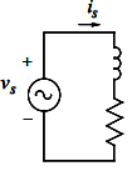
\includegraphics{2Marco/CargaRL}
\caption{ Circuito RL  } 
\label{fig:RL}
\end{figure} 


%\begin{equation}\label{eq1}
%E_{c}=\frac{1}{2}m v^2\\
%\end{equation}
%Donde:\\\\
%$E_{c}$: Energía Cinética\\
%$m$: Masa Propia Del Aire\\
%$v$: Velocidad Propia Del Aire.\\


\section{Distorción armónica total (THD) y valor RMS de la corriente distorsionada}


Una señal de corriente sinusoidal para una carga lineal como en \ref{fig:RL}, no tiene distorsión, sin embargo, hay señales de corrientes que su forma de onda es distorsionada, esto se debe a los equipos generadores de armónicos mencionados en el primer indice. \cite{A29} Un ejemplo de una señal con distorsión se puede ver en \ref{fig:distorsion_current} en donde $i_{s}$ es la señal de corriente distorsionada y $V_{s}(t)$ es sinusoidal. El análisis se aplica a la utilidad de suministros ya sean en monofásico o trifásico, en donde el estudio se realiza por fases.\\
  
\begin{figure}[H]
\centering
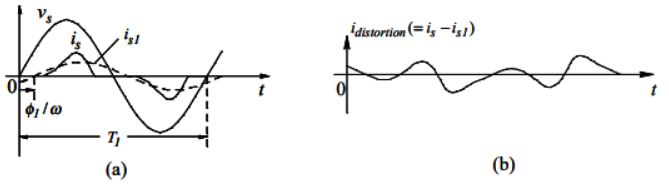
\includegraphics{2Marco/distorsin}
\caption{ Señal de corriente con distorsión (a) Fase de la corriente y su componente fundamental; (b) Componente de distorsión} \cite{A29} 
\label{fig:distorsion_current}
\end{figure} 



La onda periódica de la corriente $i_{s}(t)$, se puede expresar en componentes de Fourier:\\
\begin{equation}\label{EQ4}
i_{s}(t)=i_{s1}(t) + \sum_{h=2}^{\infty}i_{sh(t)}\\
\end{equation}
Donde:\\
$\sum_{h=2}^{\infty}i_{sh(t)} = i_{distorsion}(t)$\\

El componente dc se asume como cero e $i_{s}$ es la componente fundamental mostrada en \ref{fig:distorsion_current}(a). Partiendo de la ecuación \ref{EQ4} la componente de distorsión en la corriente es la diferencia entre $i_{s}(t)$ y su componente de frecuencia fundamental:\cite{A29}\\  
 
\begin{equation}\label{EQ5}
i_{distorsión}(t)=i_{s}(t)-i_{s1}(t)\\
\end{equation}

En una forma de onda con su frecuencia de línea $f_{1}$ y su tiempo de periodo $T_{1}(=\frac{1}{f_{1}})$, los componentes en la expresión de \ref{EQ5} son en los múltiplos de $h$ en la frecuencia fundamental, como por ejemplo, el $3^{er}$ armónico $(h=3)$ está en $180 Hz$ con un sistema de $60 Hz$.\cite{A29}\\

Un concepto básico que se usa es que en una forma de onda repetitiva, la integral de el producto de dos componentes armónicos (incluyendo la fundamental) en frecuencias desiguales sobre repeticiones del tiempo de periodo es igual a cero: \cite{A29}\\

\begin{equation}\label{EQ6}
\int_{T_{1}}^{}f_{h1}(t) \cdot g_{h2}(t) \cdot dt = 0\\
\end{equation}
Donde:\\
$h1 \neq h2$\\

Con el fin de obtener el valor rms de $i_{s}(t)$ en \ref{fig:distorsion_current}(a), se aplica el concepto básico de rms:\\

\begin{equation}\label{EQ7}
I_{s}=\sqrt{\frac{1}{T_{1}}\int_{T_{1}}^{}(i_{s})^2(t) \cdot dt}\\
\end{equation}


Donde, de \ref{EQ4}\\

\begin{equation}\label{EQ8}
i^2_{s}=(i_{s1}+ (\sum_{h=2}^{\infty}i_{sh})^2 = i^2_{sh} + \sum_{h=2}^{\infty}i^2_{sh(t)} \\ 
$+ productos en términos de frecuencia de cruce$
\end{equation}

Sustituyendo \ref{EQ8} en \ref{EQ7}, con el concepto visto en la \ref{EQ6}, cada integral de las frecuencias cruzadas es igual a cero,

\begin{equation}\label{EQ9}
I_{s} = \sqrt{\frac{1}{T}\int_{T_{1}}^{}i^2_{s1}(t) \cdot dt + \sum_{h=2}^{\infty}\frac{1}{T_{1}}\int_{T1}^{}i^2_{sh}(t)\cdot dt}\\
\end{equation}
Donde:\\
$\frac{1}{T}\int_{T_{1}}^{}i^2_{s1}(t) \cdot dt = I^2_{sh1}$\\\\
$\sum_{h=2}^{\infty}\frac{1}{T_{1}}\int_{T1}^{}i^2_{sh}(t)\cdot dt = I^2_{distorsion}$\\\\
Por lo tanto,\\
\begin{equation}\label{EQ10}
I_{s} = \sqrt{I^2_{s1}+I^2_{distorsion}}\\\\
\end{equation}

Donde los valores rms del componente de la frecuencia fundamental y los componentes de distorsión son los siguientes:\\
\begin{equation}\label{EQ11}
I_{s1}=\sqrt{\frac{1}{T}\int_{T1}^{}i^2_{s1}(t) \cdot dt}\\
\end{equation}
y\\
\begin{equation}\label{EQ12}
I_{distorsion}=\sqrt{\sum_{h=2}^{\infty}\left(\frac{1}{T_{1}}\int_{T_{1}}^{}i^2_{sh}(t)\cdot dt\right)}=\sqrt{\sum_{h=2}^{}I^2_{sh}}\\\\
\end{equation}

La ecuación descrita anteriormente, presenta que el valor rms de la componente de distorsión en \ref{fig:distorsion_current} puede ser obtenido de s valores de las componentes individual de los armónicos.\cite{A29}\\

Tomando como referencia los valores rms de los componentes de la distorsión y la fundamental en la corriente $i_{s}(t)$, un indice de distorsión llamado Distorsión Armónica Total (THD) es definida en porcentaje y este mismo pude ser presentado en distintas formas bajo las siguientes ecuaciones:\\

\begin{equation}\label{EQ13}
\%THD = 100*\frac{I_{distorsion}}{I_{s1}}\\
=100*\frac{\sqrt{I^2_{s}-I^2_{s1}}}{I_{s1}}\\
=100*\frac{\sqrt{\sum_{h=2}^{\infty}I^2_{sh}}}{I_{s1}}\\
\end{equation}



\section{ Definiciones del STD IEEE 1459 para la medición de calidad energética bajo condiciones balanceadas y des balanceadas }
\subsection{Mono-fase}
\subsubsection{Mono-fase sinusoidal}

Se parte de una entrada de tipo sinusoidal:\\
\begin{equation}\label{EQ14}
v=\sqrt{2}V sin(\omega t)\\
\end{equation}

Y si a esta, se le conecta una carga lineal, se producirá una corriente sinusoidal de tipo:\\

\begin{equation}\label{EQ15}
i\sqrt{2}I sin(\omega t - \theta)\\
\end{equation}

Donde:\\
$V$ es el valor rms de el voltaje $(V)$\\
$I$ es el valor rms de el voltaje $(I)$\\
$\omega$ es la frecuencia angular  $2\pi f(rad/s)$\\
$f$ es la frecuencia del sistema $(Hz)$\\
$\theta$ es el ángulo de fase entre el voltaje y la corriente  $(rad)$\\
$t$ es el tiempo $(s)$\\
\subsubsection{Potencia activa(W)}

La potencia activa P o también conocida como potencia real, es la medición del flujo de energía durante in intervalo de tiempo $\tau$ a $\tau + KT$. \cite{A30}\\

\begin{equation}\label{EQ16}
P=\frac{1}{KT}\int_{\tau}^{\tau + KT}pdt = \frac{1}{KT}\int_{\tau}^{\tau + KT}p_{a}dt\\
\end{equation}

Donde:\\
$T=1/f$ es el ciclo de tiempo $(s)$\\
$k$     es un número entero positivo $(s)$\\
$\tau$  es el momento cuando empieza la medición $(s)$\\
$P=VIcos \theta$\\
\subsubsection{Potencia Reactiva (var)}

La magnitud de la potencia reactiva $Q$ iguala la amplitud de la potencia reactiva instantánea $P_{q}$.\cite{A30}\\
\begin{equation}\label{EQ17}
Q=VIsin \theta\\
\end{equation}
\begin{equation}\label{EQ18}
Q=\frac{\omega}{KT}\int_{\tau}^{\tau + KT}i\left[\int_{}^{}vdt\right] dt\\
\end{equation}

Sí la carga es inductiva, entonces $Q>0$. Sí la carga es capacitiva, entonces $Q<0$. Por lo tanto, cuando la corriente atrasa el voltaje $\theta>0$ y viceversa.\\
\subsubsection{Potencia Aparente (VA)}

La potencia aparente $S$ es el producto del voltaje rms y corriente rms.\cite{A30}\\

\begin{equation}\label{EQ19}
S=VI
\end{equation}

$S=\sqrt{P^2+Q^2}$ \\

La potencia aparente de una carga monofásica se puede interpretar como la potencia activa total que se puede transmitir a través de la misma línea mientras se mantiene el voltaje rms constante de la carga y a línea de alimentación  de pérdida de potencia constante.\cite{A30}\\

\subsubsection{Factor de potencia}

\begin{equation}\label{EQ20}
PF=\frac{P}{S}
\end{equation}

El factor de potencia se puede interpretar como el radio entre la energía transmitida a la carga sobre la energía máxima que podría transmitirse, siempre y cuando las pérdidas de línea se mantengan iguales.\cite{A30}\\

Para un $S$ y $V$ dados, la utilización máxima de la línea es obtenida cuando $P=S$, por lo tanto, el radio $P/S$ es un indicador de factor de utilización.\cite{A30}\\
 \subsubsection{Potencia Compleja (VA)}
 
 La potencia compleja es una cantidad la cual la potencia activa es la parte real y la potencia reactica es la parte imaginaría.\cite{A30}\\
 
 \begin{equation}\label{EQ21}
 S = P+jQ =  VI^*\\
\end{equation}  

Esta expresión proviene del triángulo de potencias $S,P$ Y $Q$. En la figura \ref{fig:triangulo} se observa un resumen de las direcciones del flujo de potencia. El ángulo $\theta$ es el ángulo de fase de la impedancia equivalente compleja $Z/ \theta = \textbf{V/I}$.\cite{A30}\\ 

\begin{figure}[H]
\centering
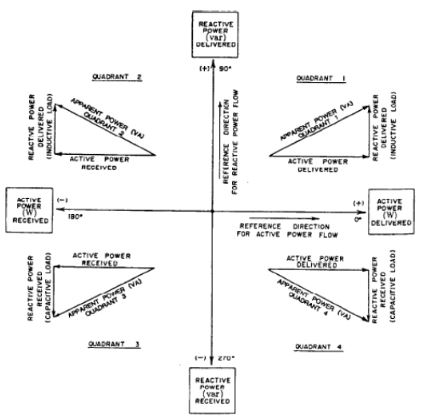
\includegraphics{2Marco/triangulopotencias}
\caption{ Cuatro cuadrantes de las direcciones del flujo de potencia} \cite{A30} 
\label{fig:triangulo}
\end{figure} 


\subsection{Mono-fase no sinusoidal}

Para condiciones estables, una señal de corriente o voltaje no sinusoidal periódica, tiene dos componentes distintos: Los componentes del sistema de frecuencia $V_{1}$ e $i_{1}$ y el termino restante $v_{H}$ e $i_{H}$.\cite{A30}\\

\begin{equation}\label{EQ22}
v=v_{1}+v_{H} 
\end{equation}
e\\\\
$i=i_{1}+i_{H}$\\\\
Donde:\\\\
$v_{1}=\sqrt{2V_{1}}sin(\omega t - \alpha_{1})$\\\\
$i_{1}=\sqrt{2I_{1}}sin(\omega t - \beta_{1})$\\\\
$v_{H}=V_{0}+\sqrt{2}\sum_{h\neq 1}^{}V_{h}sin(h\omega t-\alpha_{h})$\\\\
$i_{H}=I_{0}+\sqrt{2}\sum_{h\neq 1}^{}I_{h}sin(h\omega t-\beta_{h})$\\\\

Los valores valores rms al cuadrado son los siguientes:

\begin{equation}\label{EQ59}
\begin{split}
V^2 = {V_{1}}^2 + {V_{H}}^2 \\
I^2 = {I_{1}}^2 + {I_{H}}^2
\end{split}
\end{equation}

Las formas de ondas distorsionadas de a menudo contienen componentes de frecuencias llamadas armónicos. Un grupo especial de inter-armónicos es caracterizado por $h<1$. Estos armónicos tienen periodos más largos que el periodo $T$ de la frecuencia fundamental.\cite{A30}\\

Si la onda de corriente o voltaje distorsionada está compuesta únicamente, la medición en intervalos de tiempo $kT$, no permitirá una medición correcta de rms y valores de potencia. \cite{A30}\\

Si al menos uno de los inter-armónicos de orden $h$ es irracional, la onda observada no es periódica. En tal caso las mediciones deberían ser infinitas con el fin de tener una medición correcta del rms y las potencias.\cite{A30}\\

\subsubsection{Distorsión Total Armónica (THD) } 

La desviación en general de una onda distorsionada, se puede estimar con la ayuda de la distorsión armónica total. La distorsión armónica total del voltaje es el siguiente:\\

\begin{equation}\label{EQ23}
THD_{v}=\frac{V_{H}}{V_{1}}=\sqrt{\left(\frac{V}{V_{1}}\right)^2-1}\\
\end{equation}

La distorsión armónica total de corriente es el siguiente:\\
\begin{equation}\label{EQ24}
THD_{I}=\frac{I_{H}}{I_{1}}=\sqrt{\left(\frac{I}{I_{1}}\right)^2-1}\\
\end{equation}

\subsubsection{Potencia Activa (W)}

\begin{equation}\label{EQ25}
P=\frac{1}{kT}\int_{\tau}^{\tau + kT}pdt=\int_{\tau}^{\tau + kT}p_{a}dt\\
\end{equation}
$P=P_{1}+P_{H}$\\

\subsubsection{Potencia activa fundamental (W)}


\begin{equation}\label{EQ26}
P_{1}=\frac{1}{kT}\int_{\tau}^{\tau + kT}v_{1}i_{1}dt=V_{i}I_{1}cos \theta_{1}
\end{equation}

\subsubsection{Potencia Aparente (VA)}

\begin{equation}\label{EQ27}
S=VI\\
\end{equation}

La potencia aparente es la cantidad de potencia activa que pueden ser suministradas a la carga en condiciones ideales.\cite{A30}\\

\subsubsection{Potencia aparente fundamental (VA)}

La potencia fundamental $S_{1}$ y sus componentes $P_{1}$ y $Q_{1}$ son las cantidades actuales que ayudan a definir el tipo de flujo del campo magnético asociado con el voltaje y la corriente fundamental.\cite{A30}\\

\begin{equation}\label{EQ28}
S_{1}=V_{1}I{1}
\end{equation}

\subsubsection{Potencia Aparente no fundamental}

\begin{equation}\label{EQ29}
S_{N}=\sqrt{S^2-S^2_{1}}
\end{equation}

También se puede expresar mediante la siguiente ecuación:

\begin{equation}\label{EQ30}
S^2_{N}=D^2_{I}+D^2_{V}+S^2_{H}\\
\end{equation}

\subsubsection{Potencia de la Distorsión de Corriente (var)}
\begin{equation} \label{EQ60}
D_{1}=V_{1}I_{H}=S_{1}(THD_{I})
\end{equation}

\subsubsection{Potencia de la Distorsión de Volatje (var)}
\begin{equation} \label{EQ61}
D_{v}=V_{H}I_{1}=S_{1}(THD_{V})
\end{equation}

\subsubsection{Potencia de la Armónica Aparente (VA)}
\begin{equation} \label{EQ62}
S_{H}=V_{H}I_{H}=S_{1}(THD_{I})(THD_{V})
\end{equation}


\subsubsection{Potencia de distorsión armónica (var)}

\begin{equation}\label{EQ31}
D_{H}=\sqrt{S^2_{H}-P^2{H}}\\
\end{equation}

\subsubsection{Potencia no activa (var)}

\begin{equation}\label{EQ32}
N=\sqrt{S^2-P^2}\\
\end{equation}

Esta potencia agrupa componentes no activas fundamentales y no fundamentales.\cite{A30}\\

\subsubsection{Factor de potencia fundamental}

\begin{equation}
P_{F1}=cos \theta_{1} = \frac{P_{1}}{S_{1}}\\
\end{equation}

Este radio, facilita la evaluación de las condiciones del flujo energía.\cite{A30}\\

\subsubsection{Factor de potencia}

\begin{equation}\label{EQ33}
PF=\frac{P}{S}
\end{equation}

Dados un $S$ y un $V$, la máxima utilización de la línea es obtenido cuando $P=S$, por lo tanto, el radio $P/S$ es un indicador de factor de utilización.\cite{A30}\\

Cuando el $THD_{v}<5\%$ y $THD_{i}>40\%$, es conveniente usar la siguiente ecuación:\\

\begin{equation}\label{EQ34}
PF=\frac{1}{\sqrt{1+THD^2_{I}}}PF_{1}\\
\end{equation}

\subsection{Ejemplo monofásico}

En un circuito de alimentación monofásico se tienen las siguientes medidas tomadas por un analizador de redes eléctricas: $V_{Total}=120 V$;  $THD_{i}= 45\%$; $THD_{v}= 4\%$; $S_{1}= 200 + j40 VA$.\\

Estimar de acuerdo a los criterios de la norma IEEE 1459 las magnitudes de los siguientes parámetros: $V_{1}$, $I_{1}$, $P_{1}$, $Q_{1}$, $S_{T}$, $P_{T}$, $V_{h}$, $I_{h}$, $D_{V}$, $D_{i}$, $S_{h}$.\\

Según la ecuación \ref{EQ19}:\\

$S_{1} = \sqrt{P^2 + Q^2}; \;\;\;\;\;\; S_{1} = \sqrt{200^2 + 40^2} $\\

\textbf{* }$S_{1} = 203,9608 VA$\\

Según la ecuación \ref{EQ23}:\\

$THD_{v}=\sqrt{\left(\frac{V}{V_{1}}\right)^2-1} ;  \;\;\;\;\;\; {THD_{v}}^2=\left(\frac{V}{V_{1}}\right)^2 - 1;  \;\;\;\;\;\;
{THD_{v1}}^2=\frac{{V}^2 - {{V}_{1}}^2}{{V_{1}}^2} $\\

${THD_{v1}}^2*{{V_{1}}^2}={{V}^2 - {{V}_{1}}^2}; \;\;\;\;\;\;
{THD_{v1}}^2*{{V_{1}}^2} + {{V}_{1}}^2={{V}^2}; \;\;\;\;\;\;
{V_{1}}^2 ({THD_{v1}}^2 + 1)={{V}^2}; \;\;\;\;\;\;$\\

${V_{1}}^2 = \frac{{{V}^2}}{{THD_{v1}}^2 + 1}; \;\;\;\;\;\;
V_{1} = \sqrt{\frac{{{V}^2}}{{THD_{v1}}^2 + 1}}; \;\;\;\;\;\;
V_{1} = \sqrt{\frac{{{120V}^2}}{{0.04}^2 + 1}}$\\

\textbf{* }$V_{1} = 119.9041V$\\

$V_{H} = THD_{v}*V_{1};  \;\;\;\;\;\;
V_{H} = 0.04 * 119.9041V$\\

\textbf{* }$V_{H} = 4,7962 V$\\

Según la ecuación \ref{EQ28}:\\

$S_{1} = V_{1}*I_{1}; \;\;\;\;\;\;
I_{1} = \frac{S_{1}}{V_{1}}; \;\;\;\;\;\;
I_{1} = \frac{203,9608VA}{119,9041V}$\\

\textbf{* }$I_{1} = 1,7010A$\\

$I_{H} = THD_{I} * I_{1}; \;\;\;\;\;\;
I_{H} = 0,45 * 1,7010A$\\

\textbf{* }$I_{H} = 0,7654A$\\

Según la ecuación \ref{EQ59}:\\

$I^2 = {I_{1}}^2 + {I_{H}}^2; \;\;\;\;\;\;
I = \sqrt{{I_{1}}^2 + {I_{H}}^2}; \;\;\;\;\;\;
I = \sqrt{{1,7010A}^2 + {0,7654A}^2}$\\

\textbf{* }$I = 1,8653A$\\

Según la ecuación \ref{EQ28}: \\

$S = V*I; \;\;\;\;\;\;
S = 119,9041V * 1,8653A$\\

\textbf{* }$S = 223,836VA$\\

$S_{H} = V_{H}*I_{H}; \;\;\;\;\;\;
\textbf{* }S_{H} = 4,7962V * 0,7654A = 3,6710VA$\\

Según la ecuación \ref{EQ29}: \\

$S_{N} = \sqrt{{S}^2 - {{S}_{1}}^2}; \;\;\;\;\;\;
S_{N} =  \sqrt{{223,836VA}^2 - {203,9608VA}^2}$\\

\textbf{* }$S_{N} = 92,2094VA$\\

Según la ecuación \ref{EQ60}: \\

\textbf{* }$D_{1} = V_{1}*I_{H} = 119,9041V * 0,7654A = 91,7745VA$\\

\textbf{* }$D_{v} = V_{H}*I_{1} = 4.7962V *1,7010A = 8,1583VA$\\

Según la ecuación \ref{EQ26}: \\

$P_{1} = V_{1}*I_{1}*cos \theta_{1}; \;\;\;\;\;\; 
\theta_{1} =  cos^{-1}(\frac{P_{1}}{V_{1}*I_{1}}); \;\;\;\;\;\; 
\theta_{1} =  cos^{-1}(\frac{200VA}{119,9041V*1,7010A})$\\

\textbf{* }$\theta_{1} = 11,3044º$\\

Según la ecuación \ref{EQ33}: \\

$PF_{1} = \frac{P_{1}}{S_{1}}; \;\;\;\;\;\; PF_{1} = \frac{203,9608VA}{200VA};$\\

\textbf{* }$PF_{1} = 0,9805$

Según la ecuación ref{EQ34}: \\

$PF=\frac{1}{\sqrt{1+THD^2_{I}}}PF_{1}; \;\;\;\;\;\; PF=\frac{1}{\sqrt{1+0,45^2}}0,9805$ \\

\textbf{* } $PF= 0,8941$

Según la ecuación \ref{EQ33}: \\

$PF= \frac{P}{S}; \;\;\;\;\;\; P = PF * S; \;\;\;\;\;\; P = 0,8941 * 223,836 VA$\\

\textbf{* } $P = 200,1317VA$ \\

Según la ecuación \ref{EQ32}: \\

$N=\sqrt{S^2-P^2}; \;\;\;\;\;\; \sqrt{223,836VA^2-200,1317VA^2}$\\

\textbf{* }$N = 100,2489 VAR$\\

Según la ecuación \ref{EQ25}: \\

$P_{H} = P - P_{1}; \;\;\;\;\;\;\; P_{H} = 200,1317VA - 200VA$\\

\textbf{* }$P_{H} = 0,1317VA$

Según la ecuación \ref{EQ31}: \\

$D_{H}=\sqrt{S^2_{H}-P^2{H}}; \;\;\;\;\;\;\; D_{H} = \sqrt{3,6710VA^2 - 0,1317VA^2}$\\

\textbf{* }$D_{H} = 3,6686VAR$

\subsection{Sistema trifásico sinusoidal balanceado }

Para este caso se asume un sistema de secuencia positiva rotativa en sentido anti-horario, a, b, c, lo voltaje linea a neutro son los siguientes:

\begin{equation}\label{EQ35}
v_{a}=\sqrt{2}V sin(\omega t)\\
\end{equation} 
$v_{b}=\sqrt{2}V sin(\omega t-120^{\circ})$\\
$v_{c}=\sqrt{2}V sin(\omega t+120^{\circ})$\\

Las líneas de corriente tienen ecuaciones similares, las cuales son:

\begin{equation}\label{EQ36}
i_{a}=\sqrt{2}I sin(\omega t-\theta)\\
\end{equation} 
$i_{b}=\sqrt{2}I sin(\omega t-\theta -120^{\circ})$\\
$i_{c}=\sqrt{2}I sin(\omega t-\theta +120^{\circ})$\\

En sistemas trifásicos balanceados y perfectamente sinusoidal, los sistemas de bajo voltaje no son comunes, solo bajo condiciones de laboratorio en donde se usan amplificadores de potencia de baja distorsión.\cite{A30}\\

En el caso de un sistemas de tres líneas, con voltajes línea a neutro son definidas asumiendo un nodo neutral artificial, el cual se obtienen con ayuda de tres resistencias idénticas conectadas en \textbf{Y}.

\subsubsection{Potencia activa (w)} 
\begin{equation}\label{Eq37}
P=\frac{1}{kT}\int_{\tau}^{\tau +kT}pdt\\
\end{equation}
$P=3VI\cos\theta=\sqrt{3}V_{\ell \ell}I\cos\theta$\\
Donde\\
$V$              es el voltaje rms de línea a neutro\\
$V_{\ell \ell}$  es el voltaje rms línea a línea\\

\subsubsection{Potencia reactiva}


\begin{equation}\label{EQ38}
Q=3VI\sin\theta=\sqrt{3}V_{\ell \ell}I\sin\theta\\
\end{equation}
$|Q|=\sqrt{S^2-P^2}$\\

\subsubsection{Potencia aparente}

\begin{equation}\label{EQ39}
S=3VI=\sqrt{3}V_{\ell \ell}I\\
\end{equation}

\subsubsection{Factor de potencia}

\begin{equation}\label{EQ40}
PF=\frac{P}{s}\\
\end{equation}

\subsection{Sistema trifásico sinusoidal no balanceada}

En este caso, los tres hilos de corriente \textbf{$I_{a},I_{b}$} y \textbf{$I_{c}$}, no tienen las mismas magnitudes y no están desplazadas exactamente $120^{\circ}$ con respecto una a la otra. Las cargas no balanceadas  conlleva a corrientes asimétricas que a su vez causan asimetría de voltaje. En algunas ocasiones sucede que los tres fasores de voltaje no son simétricos. Esto conduce a corrientes asimétras incluso cuando la carga está perfectamente balanceada.\cite{A30}\\


Las ecuaciones de voltaje línea a neutro son los siguientes:

\begin{equation}\label{EQ41}
v_{a}=\sqrt{2}V_{a}\sin(\omega t+\alpha_{a})\\
\end{equation}
$v_{b}=\sqrt{2}V_{b}\sin(\omega t+\alpha_{b} -120^{\circ})$\\\\
$v_{c}=\sqrt{2}V_{c}\sin(\omega t+\alpha_{c}+120^{\circ})$\\\\
Donde por lo menos una de las tres amplitudes linea a neutro $\sqrt{2}V_{q},\sqrt{2}V_{b},$ o $\sqrt{2}V_{c}$ tiene un valor diferente que al de las otras dos amplitudes. Lo mismo debe aplicar a los ángulos de las fases $\alpha_{a}, \alpha_{b},$ y $\alpha_{c}$. Si un ángulo de fase tiene un valor distinto que los otros dos, el sistema está perdiendo simetría y no es balanceado.\cite{A30}\\


Las ecuaciones de corriente línea a neutro son los siguientes:

\begin{equation}\label{EQ41}
i_{a}=\sqrt{2}I_{a}\sin(\omega t+\beta_{a})\\
\end{equation}
$i_{b}=\sqrt{2}I_{b}\sin(\omega t+\beta_{b} -120^{\circ})$\\\\
$i_{c}=\sqrt{2}i_{c}\sin(\omega t+\beta_{c}+120^{\circ})$\\\\

\subsubsection{Potencia Activa}

\begin{equation}\label{EQ42}
P=\frac{1}{kT}\int_{\tau}^{\tau +kT}pdt\\
\end{equation}
$P=P_{a}+P_{b}+P_{c}$\\\\

Donde $P_{a},P_{b}$ y $P_{c}$ son potencias de fases activas:

\begin{equation}\label{EQ43}
P_{a}=\frac{1}{kT}\int_{\tau}^{\tau +kT}v_{a}i_{a}dt=V_{a}I_{a}\cos\theta_{a};\\ \theta_{a}=\alpha_{a}-\beta_{a}\\
\end{equation}
$P_{b}=\frac{1}{kT}\int_{\tau}^{\tau +kT}v_{b}i_{b}dt=V_{b}I_{b}\cos\theta_{b};$ \hspace{1.5cm} $\theta_{b}=\alpha_{b}-\beta_{b}$\\\\
$P_{c}=\frac{1}{kT}\int_{\tau}^{\tau +kT}v_{c}i_{c}dt=V_{c}I_{c}\cos\theta_{c};$ \hspace{1.5cm} $\theta_{c}=\alpha_{c}-\beta_{c}$\\\\


\subsubsection{Potencias activa en secuencias positivas, negativas y cero (w)}

En sistemas de cuatro hilos, hay situaciones cuando el uso componentes simétricos pueden ser de ayuda. Los componentes simétricos de voltaje $V^{+},V^{-}$ y $V_{0}$ y las componentes de corriente $I^{+},I^{-}$  e $I_{0}$ con sus respectivos ángulos $\theta^{+},\theta^{-}$ y $\theta^{0}$ producen los siguientes tres componentes de potencia activa:\cite{A30}\\

La potencia de secuencia positiva:\\


\begin{equation}\label{EQ44}
P^+=3V^{+}I^{+}\cos\theta^{+}\\
\end{equation} 
La potencia de secuencia negativa:\\


\begin{equation}\label{EQ45}
P^-=3V^{-}I^{-}\cos\theta^{-}\\
\end{equation} 
La potencia de secuencia cero:\\


\begin{equation}\label{EQ46}
P^0=3V^{0}I^{0}\cos\theta^{0}\\
\end{equation} 

La potencia activa total es:

\begin{equation}\label{EQ47}
P=P^{+}+P^{-}+P^{0}\\
\end{equation}

\subsubsection{Potencia reactiva (var)}

Las potencias reactivas por fase son definidas con la ayuda de las siguientes ecuaciones:

\begin{equation}\label{EQ48}
Q_{a}=\frac{\omega}{kT}\int_{\tau}^{\tau +kT}i_{a}\left[\int_{}^{}v_{a}dt\right]dt=V_{a}I_{a}\sin\theta_{a}\\
\end{equation}
$Q_{b}=\frac{\omega}{kT}\int_{\tau}^{\tau +kT}i_{b}\left[\int_{}^{}v_{b}dt\right]dt=V_{b}I_{b}\sin\theta_{b}$\\\\

$Q_{c}=\frac{\omega}{kT}\int_{\tau}^{\tau +kT}i_{c}\left[\int_{}^{}v_{c}dt\right]dt=V_{c}I_{c}\sin\theta_{c}$\\\\

La potencia reactiva total es:\\

\begin{equation}\label{EQ50}
Q=Q_{a}+Q_{a}+Q_{c}\\
\end{equation}

\subsubsection{Potencias aparentes en fase}

\begin{equation}\label{EQ51}
S_{a}=V_{a}I_{a}; \hspace{1cm} S_{b}=V_{b}I_{b}; \hspace{1cm} S_{c}=V_{c}I_{c}\\
\end{equation}
$S^2_{a}=P^2_{a}Q^2_{a};$ \hspace{1cm} $S^2_{b}=P^2_{b}Q^2_{b};$ \hspace{1cm} $S^2_{c}=P^2_{c}I_{c}$\\

\subsubsection{Potencia aparente aritmética }

\begin{equation}\label{EQ52}
S_{A}=S_{a}+S_{b}+S_{c}\\
\end{equation}

$S_{A} \neq \sqrt{P^2+Q^2}$

\subsubsection{Potencia aparente del vector}

\begin{equation}\label{EQ53}
S_{V}=\sqrt{P^2+Q^2}\\
\end{equation}

En la Fig \ref{fig:inter}, se muestra un interpretación de $S_{V}$ y $S_{A}$.

\begin{figure}[H]
\centering
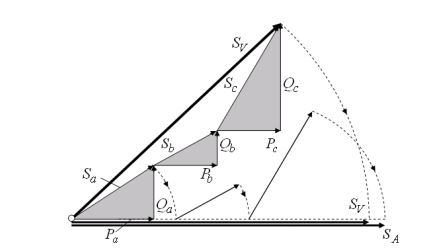
\includegraphics{2Marco/intergeo}
\caption{Potencias aparentes aritmpeticas y de vector} 
\label{fig:inter}
\end{figure} 

\subsubsection{Factor de potencia aritmético y del vector }

\begin{equation}\label{EQ54}
PF_{V}=\frac{P}{S_{V}}\\
\end{equation}
$PF_{A}=\frac{P}{S_{A}}$\\

Una línea trifásica que abastece a uno o más clientes debería ser vista como un solo camino, una entidad que transmite la energía eléctrica a lugares donde es convertida en otras forma de energía. Esta mal ver cada fase como una ruta de energía independiente.\cite{A30}\\

\subsubsection{Potencia aparente efectiva}

Este concepto asume un circuito balanceado virtual que tiene exactamente las mismas líneas de perdidas como el circuito des balanceado actual. Para un sistema de 4 líneas, el balance de la perdida de potencia es expresado en la siguiente ecuación:\cite{A30}\\

\begin{equation}\label{EQ55}
r(I^2_{a}+I^2_{b}+I^2_{c}+\rho I^2_{n})=3rI^2_{e}\\
\end{equation}
Donde:\\\\
$r$			es la resistencia\\
$I_{n}$		es la corriente actual (rms)\\
$r_{n}$		Es el cable neutro de la resistencia\\

De las ecuaciones anteriores, la corriente equivalente de un sistema de 4 líneas es el siguiente:\\

\begin{equation}\label{EQ56}
I_{e}=\sqrt{\frac{I^2_{a}+I^2_{b}+I^2_{c}+\rho I^2_{n}}{3}}=\sqrt{(I^+)^2+(I^-)^2+(1+3\rho)(I^0)^2}\\
\end{equation}

Y para un sistema de tres hilos donde $I^0=0$\\

\begin{equation}\label{EQ57}
I_{e}=\sqrt{\frac{I^2_{a}+I^2_{b}+I^2_{c}}{3}}=\sqrt{(I^+)^2+(I^-)^2}\\
\end{equation}

\subsubsection{Factor de potencia efectiva}

\begin{equation}\label{EQ58}
PF_{e}=\frac{P}{S_{e}}\\
\end{equation}

\section{Ejercicio Práctico}

\subsection{Análisis de datos obtenidos de tres cargas no lineales}

A continuación, se muestra el análisis de los datos obtenidos por el circutor de tres computadores de los etm de la Universidad Santo Tomas en la sede central, siguiendo las normas establecidas para cada caso a nivel nacional. \\
El circutor no posee una memoria que almacene los datos medidos, por tal razón, los datos obtenidos se transmiten en tiempo real por comunicación serial a un computador por medio de un programa realizado en Visual Studio, donde se pueden adquirir las medidas de potencia, tensiones, voltajes, THDi, THDv, en una hoja de cálculo.\\
Las medidas tomadas y el análisis de estas, se realizaron tomando como referencia la norma NTC 1340 (tercera actualización) y el IEEE 1159, el cual establece el tiempo de muestreo para el monitoreo de calidad de energía eléctrica que es mayor a un minuto para sistemas de larga duración en variaciones de rms.

\begin{table}
\begin{center}
\begin{tabular}{ |c|c|c|c|c|c|c|c|c| } 
\hline
Nombre & Fecha & Hora & Prom & Min & Max & Muestras & Duración & Unidades\\
\hline
Frecuencia & 18/05/2018 & 18:13 & 60 & 60 & 60 & 30 & 6:00 & min:s\\
\hline
\end{tabular}
\end{center}
\caption{Datos de caracterización de frecuencia}
\label{tab:ejercicio-frecuencia}
\end{table}



\begin{figure}[H]
\centering
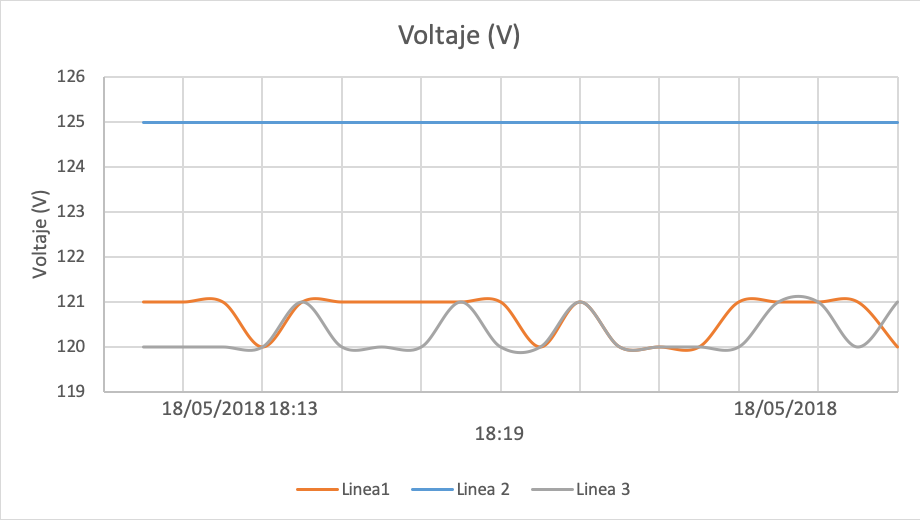
\includegraphics{2Marco/voltaje-rms}
\caption{Voltaje RMS} 
\label{fig:voltaje-rms}
\end{figure} 

Según la norma NTC 1340 (Tercera actualización) expresa que el 100\% de los valores medidos en el rango establecido del IEEE 1159, deben estar dentro del intervalo definido en la figura \ref{fig:tension-nominal}

\begin{figure}[H]
\centering
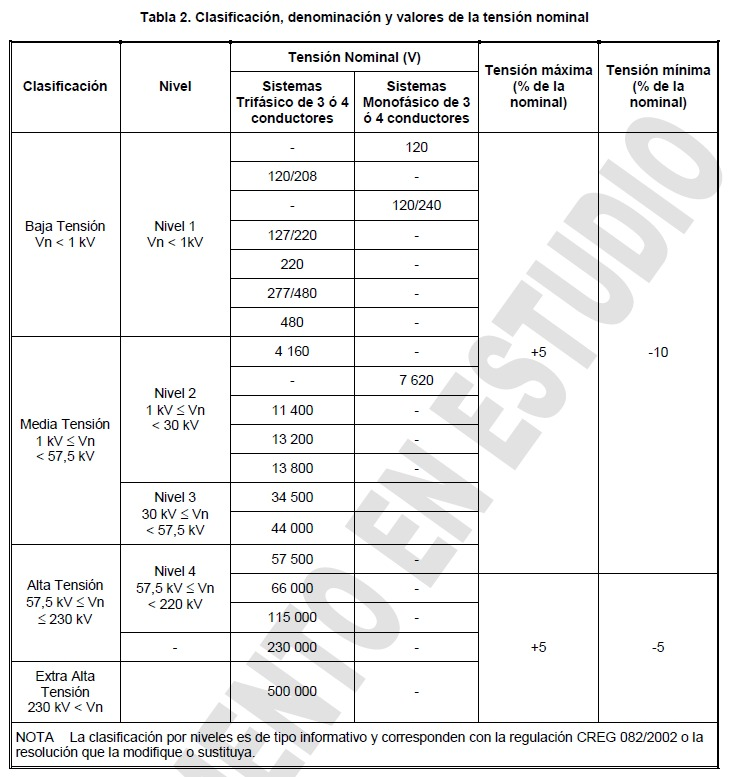
\includegraphics{2Marco/tension-nominal}
\caption{Clasificación, denominación y valores tensión nominal} 
\label{fig:tension-nominal}
\end{figure} 

Con los valores de la figura \ref{fig:voltaje-rms} se evidencia que los valores máximos y mínimos de VRMS, cumplen con los porcentajes establecidos.

\begin{align*}
X1 = \frac{Vmaxl1}{120} = \frac{121}{120} = 1.008;\;\mathbf{ 0,8\% VRMS} \\\\
X2 = \frac{Vmaxl2}{120} = \frac{125}{120} = 1.041;\;\mathbf{ 4.1\% VRMS} \\\\
X3 = \frac{Vmaxl3}{120} = \frac{121}{120} = 1.008;\;\mathbf{ 0,8\% VRMS}
\end{align*}
\textbf{Porcentaje máximos de volatjes}\\
\begin{align*}
&y1 = \frac{Vminl1}{120} = \frac{120}{120} = 1.00;\;\mathbf{ 0\% VRMS} \\\\
&y2 = \frac{Vminl2}{120} = \frac{125}{120} = 1.041;\;\mathbf{ 4.1\% VRMS} \\\\
&y3 = \frac{Vminl3}{120} = \frac{120}{120} = 1.00;\;\mathbf{ 0\% VRMS}
\end{align*}
\textbf{Porcentaje mínimos de volatjes}\\

\begin{table}
\begin{center}
\begin{tabular}{ |c|c|c| } 
\hline
VRMS & MÁXIMO & MÍNIMO\\
\hline
L1V & 0.8\% & 0\%\\
\hline
L2V & 4,1\% & 4,1\%\\
\hline
L3V & 0.8\% & 0\%\\
\hline
\end{tabular}
\end{center}
\caption{Tabla de rangos máximos y mínimos de VRMS}
\label{tab:rangos-vrms}
\end{table}

Al comparar los datos de la tabla en la figura \ref{fig:tension-nominal} con la tabla \ref{tab:rangos-vrms}, se afirma que la tensión nominal de las cargas cumple con los intervalos establecidos en la norma NTC 1340.\\

\begin{table}[!htbp]
\begin{center}
\begin{tabular}{ |c|c|c|c|c|c|c|c|c| } 
\hline
Nombre & Fecha & Hora & RMS & Min & Max & Unidades & Duración & Unidades\\
\hline
L1 Irms & 18/05/2018 & 18:13 & 605,1 & 537 & 808 & mA & 6:00 & min:s\\
\hline
L2 Irms & 18/05/2018 & 18:13 & 624,1 & 576 & 790 & mA & 6:00 & min:s\\
\hline
L3 Irms & 18/05/2018 & 18:13 & 576,5 & 553 & 730 & mA & 6:00 & min:s\\
\hline
\end{tabular}
\end{center}
\caption{Datos de caracterización de corriente}
\label{tab:ejercicio-corriente}
\end{table}

\begin{figure}[H]
\centering
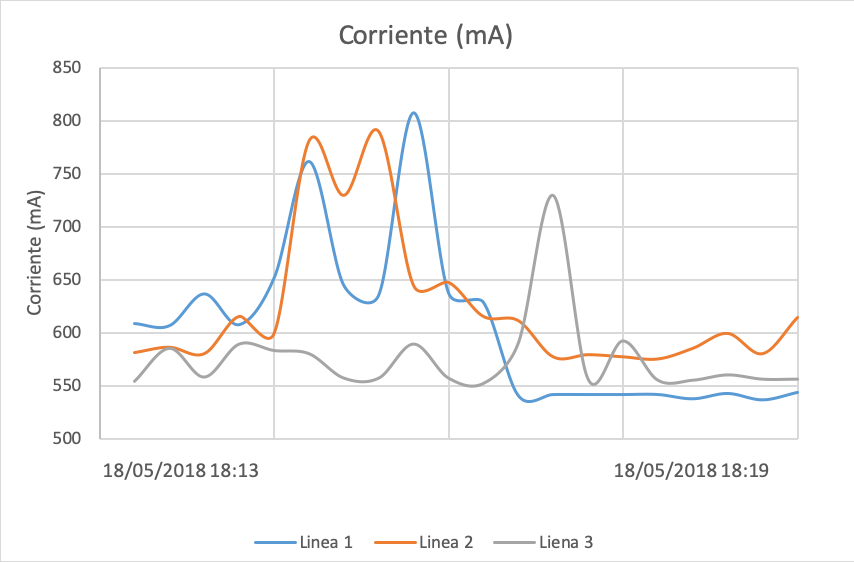
\includegraphics{2Marco/corriente-rms}
\caption{Corriente RMS} 
\label{fig:corriente-rms}
\end{figure} 

La figura \ref{fig:corriente-rms} corresponde a la corriente consumida dentro del intervalo ya establecido, se observa que los valores cambian en un rango de 300 mA, debido al uso que le aplican al computador.

\begin{table}[!htbp]
\begin{center}
\begin{tabular}{ |c|c|c|c|c|c|c|c|c| }
\hline
Nombre & Fecha & Hora & RMS & Min & Max & Unidades & Duración & Unidades\\
\hline
L1 THDv & 18/05/2018 & 18:13 & 2,9 & 2 & 3 & \% & 6:00 & min:s\\
\hline
L2 THDv & 18/05/2018 & 18:13 & 2,85 & 2 & 3 & \% & 6:00 & min:s\\
\hline
L3 THDv & 18/05/2018 & 18:13 & 2,9 & 2 & 3 & \% & 6:00 & min:s\\
\hline
L1 THDi & 18/05/2018 & 18:13 & 40,44 & 34,2 & 45,4 & \% & 6:00 & min:s\\
\hline
L2 THDi & 18/05/2018 & 18:13 & 39,75 & 25,6 & 44,9 & \% & 6:00 & min:s\\
\hline
L3 THDi & 18/05/2018 & 18:13 & 40,45 & 30,9 & 44,5 & \% & 6:00 & min:s\\
\hline
\end{tabular}
\end{center}
\caption{Distorsión armónica en corriente y voltaje}
\label{tab:distorsion-armonica}
\end{table}

\begin{figure}[H]
\centering
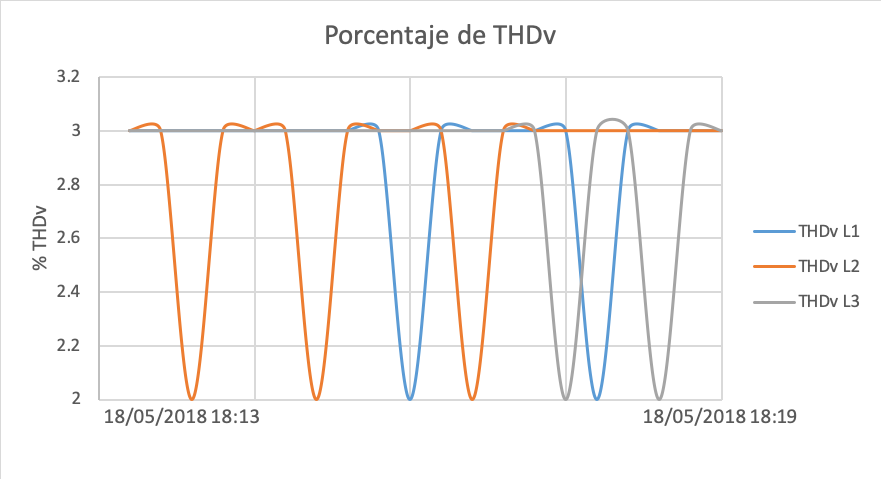
\includegraphics{2Marco/porcentaje-thdv}
\caption{Porcentaje de $THD_{V}$} 
\label{fig:porcentaje-thdv}
\end{figure} 

\begin{figure}[H]
\centering
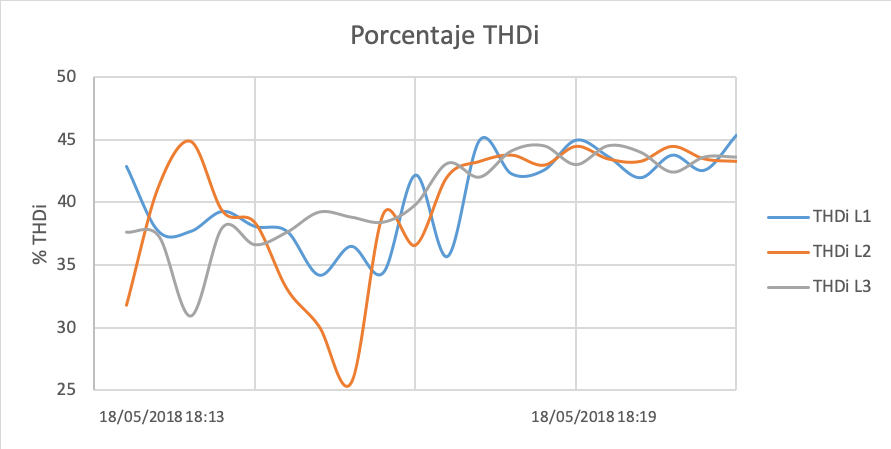
\includegraphics{2Marco/porcentaje-thdi}
\caption{Porcentaje de $THD_{I}$} 
\label{fig:porcentaje-thdi}
\end{figure} 

Los datos de distorsión armónica reflejados en la tabla \ref{tab:distorsion-armonica} y las figuras \ref{fig:porcentaje-thdv}, \ref{fig:porcentaje-thdi} dan a entender como esta afectando las cargas no lineales en el sistema. Según el estándar IEEE 519 en el capitulo 11.1 indica el límite máximo que debe tener el THD en tensión (5\%), de acuerdo en la figura \ref{fig:porcentaje-thdv}, los THD de tensión no exceden el valor indicado anteriormente, por lo tanto, la red está cumpliendo la normatividad internacional.\\ 
En los THD de corriente, para su análisis es necesario hallar la distorsión de la demanda total con la siguiente ecuación:\\

\begin{equation}\label{EQ63}
TDD=\frac{I1*THD}{IL}\\
\end{equation}
\textbf{Ecuación \ref{EQ63}. Distorsión de demanta total.}

La corriente de carga (IL1) se toma el promedio de la tabla de datos que se obtiene por medio del CIRCUTOR de la siguiente manera:

\begin{align*}
&IL1 = L1Irms\;\;\; RMS = 605.1\\
&I_{1a1} = I_{L1} - (I_{L1} * 0.4044) = 0.605 - (0.605 * 0.4044) = 0.3603
\end{align*}

Aplicando la ecuación \ref{EQ63}

\begin{align*}
TDD_{1} = \frac{I_{1a1}*THD_{1}}{I_{L1}} = \frac{0.3603*0.4044}{0.605} = 0.2408 = 24.08\%
\end{align*}

La corriente de carga (IL2) se toma el promedio de la tabla de datos que se obtiene por medio del CIRCUTOR de la siguiente manera:

\begin{align*}
&IL2 = L2Irms RMS = 624.1\\
&I_{1a2} = I_{L2} - (I_{L2} * 0.3975) = 0.624 - (0.624 * 0.3975) = 0.3760
\end{align*}

Aplicando la ecuación \ref{EQ63}

\begin{align*}
TDD_{2} = \frac{I_{1a2}*THD_{2}}{I_{L2}} = \frac{0.3760*0.3975}{0.624} = 0.2395 = 23.95\%
\end{align*}

La corriente de carga (IL3) se toma el promedio de la tabla de datos que se obtiene por medio del CIRCUTOR de la siguiente manera:

\begin{align*}
&IL3 = L3Irms RMS = 576.5\\
&I_{1a3} = I_{L3} - (I_{L3} * 0.4045) = 0576 - (0.576 * 0.4045) = 0.2330
\end{align*}

Aplicando la ecuación \ref{EQ63}

\begin{align*}
TDD_{3} = \frac{I_{1a3}*THD_{3}}{I_{L3}} = \frac{0.2330*0.4045}{0.576} = 0.1636 = 16.36\%
\end{align*}\\

\begin{table}[!htbp]
\begin{center}
\begin{tabular}{ |c|c| } 
\hline
Corrientes & TDD\\
\hline
AL1 & 24.08\%\\
\hline
AL2 & 23.95\%\\
\hline
AL3 & 16.63\%\\
\hline
\end{tabular}
\end{center}
\caption{TDD de corrientes}
\label{tab:tdd-corriente}
\end{table}

Tomando como referencia la figura \ref{fig:limites-corriente}, la cual está en el estándar IEEE 519 y la tabla \ref{tab:tdd-corriente}, se observa que los resultados de TDD obtenidos en las ecuaciones anteriores están dentro del rango aceptado en el estándar, comprobando que el sistema está trabajando en un estado estable. 

\begin{figure}[H]
\centering
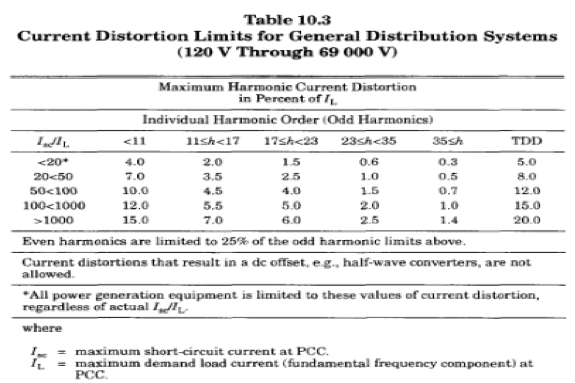
\includegraphics{2Marco/limites-distorsion-corriente}
\caption{Limites de distorsión de corriente para sistemas de distribución general} 
\label{fig:limites-corriente}
\end{figure} 

\section{Desarrollo de Software}

El desarrollo de software es un campo de la ciencia computacional dedicado a la creación, diseño, implementación y soporte de software.

El softaware se compone de una serie de instrucciones o programas que le dicen al computador que debe hacer. Es independiente del hardware y hace a los computadores programables.  \cite{A31}

\subsection{Programación Orientada a Objetos}

La programación orientada a objetos (OOP) es un paradigma de programación  basado en convertir objetos que puedan ser tangibles o intangibles a objetos digitales los cuáles tienen metodos y propiedades. Esto genera ventajas en modularidad y reusabilidad en código. Los objetos que usualmente son instancias de clases, son utilizados para interactuar uno con otro para diseñar aplicaciones y programas de computadores. \cite{A32}

\subsection{Desarrollo Web}

El desarrollo web es una área del desarrollo de software la cuál construye, crea y mantiene sitios web. Dentro de su funcionamiento incluye el diseño web, publicación web y administración de base de datos. \cite{A33}

\subsection{Frontend}

Frontend se entiende como la parte de un programa en la cuál se crea una interfaz de usuario para que el programa interactue con las personas. Los lenguajes principales desarrollo del frontend son Html5, Javascript y Css 3; aunque hay muchos frameworks facilitan la creación de frontend, cómo lo son: React, Angular2+, Vuejs y Bootsrap entre otros.

\subsection{Backend}

En la capa de arquitectura de un proyecto de software, el backend el backend no es accesible por los usuarios ya que este es el encargado de ejecutar todas las funciones y la lógica del sistema, administra y guarda y envía información a la base de datos.

\subsection{REST}

REST se compone de una serie de principios de comunicación web en la cual se diseñan servicios web orientados a recursos de sistemas, incluyendo como los estados de los recursos son ubicados y transferidos atravez del protocolo HTTP por un gran rango de clientes que usan distintos lenguajes de programación.  \cite{A37}


\section{Fourier}
\subsection{Transformada de Fourier}
La transformada de Fourier transforma una señal que depende del tiempo en una señal que depende de la frecuencia (tiempo continuo a tiempo discreto).
\begin{equation}
F(g(t))=G(f)=\int_{-\infty}^{\infty}g(t)e^{-i2\pi ft}dt   
\end{equation}
Se define como la transformada de Fourier. \cite{A34}
\begin{equation}
F^{-1}(G(f))=g(t)=\int_{-\infty}^{\infty}G(f)e^{i2\pi ft}df   
\end{equation} 
Se define como  la inversa de Fourier. \cite{A34}

\subsection{Teorema de muestreo de Nyquist-Shannon}
Sea una señal de \textit{x(t)} de  finita y de banda  limitada  a B, entonces:
\\

$x(t)=\dfrac{1}{\pi}\sum_{n=-\infty}^{\infty} x(\dfrac{n}{2B})\dfrac{\sin(\pi(2Bt-n)) }{2Bt-n}$
\cite{A35}\\

para reconstruir una señal limitada entre la banda B es necesario tener una señal de muestreo de 2B, esta frecuencia se denomina frecuencia de Nyquist.

\begin{equation}
F_{min}>2f
\end{equation}
Donde:\\
F$_{min}$ = Frecuencia mínima de muestreo.\\
f = Frecuencia fundamental de la señal.

\subsection{Transformada rápida de Fourier (FFT) }
Todas las señales periódicas pueden ser representadas en sumatorias de Fourier, de esta sumatoria de Fourier se puede sacar la transformada de Fourier discreta calculando un tiempo finito, esta transformada se define como:
\begin{equation}
X[k]=\sum_{n=0}^{N-1}x[n]W_{N}^{kn} ; \\   k = 0,1,2,3...N-1
\end{equation}
donde $W_{N}=e^{-j\dfrac{2\pi}{N}}$\\
La FFT surge en dividir el tiempo, es decir en la descomposición en transformadas de Fourier Discretas mas simples, para esto se asume que la N es potencia de 2, descomponiendo la como: 

\begin{equation}
X[k]=\sum_{r=0}^{N/2-1}x[2r](W_{N/2})^rk + W_{N}^K \sum_{r=0}^{N/2-1}x[2r+1](W_{N/2})^rk
\end{equation}

donde $W_{N/2}=e^{-j\dfrac{2\pi}{N/2}}$, N siendo el número de muestras. \cite{A36}\\

Esta manera es la que usan la mayoría de conversares análogos digitales y procesadores. 


\section{Convertidores ADC}
El convertido análogo digital (ADC) fue creado para representar en una palabra digital el nivel de voltaje existente en una en una entrada análoga, transformándola en una señal binaria de un número de muestras (N), en la electrónica la resolución de la señal de entrada la da la cantidad de bits disponibles para la conversión, entre mas grande sea la cantidad de bits, mayor es la resolución de la señal y mas confiable es esta. 

\section{Internet de las cosas}

El concepto de internet de las cosas o por su sigla en ingles (IoT) - internet of things, tiene como objetivo conectar lo desconectado, esto significa que algún dispositivo que no tenga comunicación con la red lo pueda tener y así puedan interactuar con las personas y otros objetos. IoT es una tecnología de transición en donde los dispositivos permitiran sensar y controlar el mundo fisico haciendo los objetos inteligentes y conectandolos atravez de una red inteligente. Esta transición de volver un dispositivo intelegente se puede realizar de distintas formas pero la más común para empezar es la Raspberry. \cite{A38}

\subsection{Raspberry pi 4}

Las Raspberry Pi 4 es la nueva generación de computadores soportando más memoria RAM y un mejor rendimiento en CPU, GPU y puertos de entrada y salida. Esta tarjeta cuenta con conectividad Bluetooth 2.0, USB, Red y Wifi, también tiene el protocolo de comunicación I2C el cual permite comunicarse con sistemas digitales electrónicos con el fin de recibir y transmitir información y por medio de la conectividad Wifi, se puede hacer conectividad a la red dispositivos que no tienen conectividad. El mayor beneficio de esta funcionalidad de la Raspberry hace posible el concepto de IoT y así puede haber una interacción entre las personas y los dispositivos. \cite{A39}
%\newpage{\cleardoublepage}
\chapter{Desarrollo y ejecución del proyecto}
\section{Arquitectura del proyecto}
\begin{figure}[H]
\centering
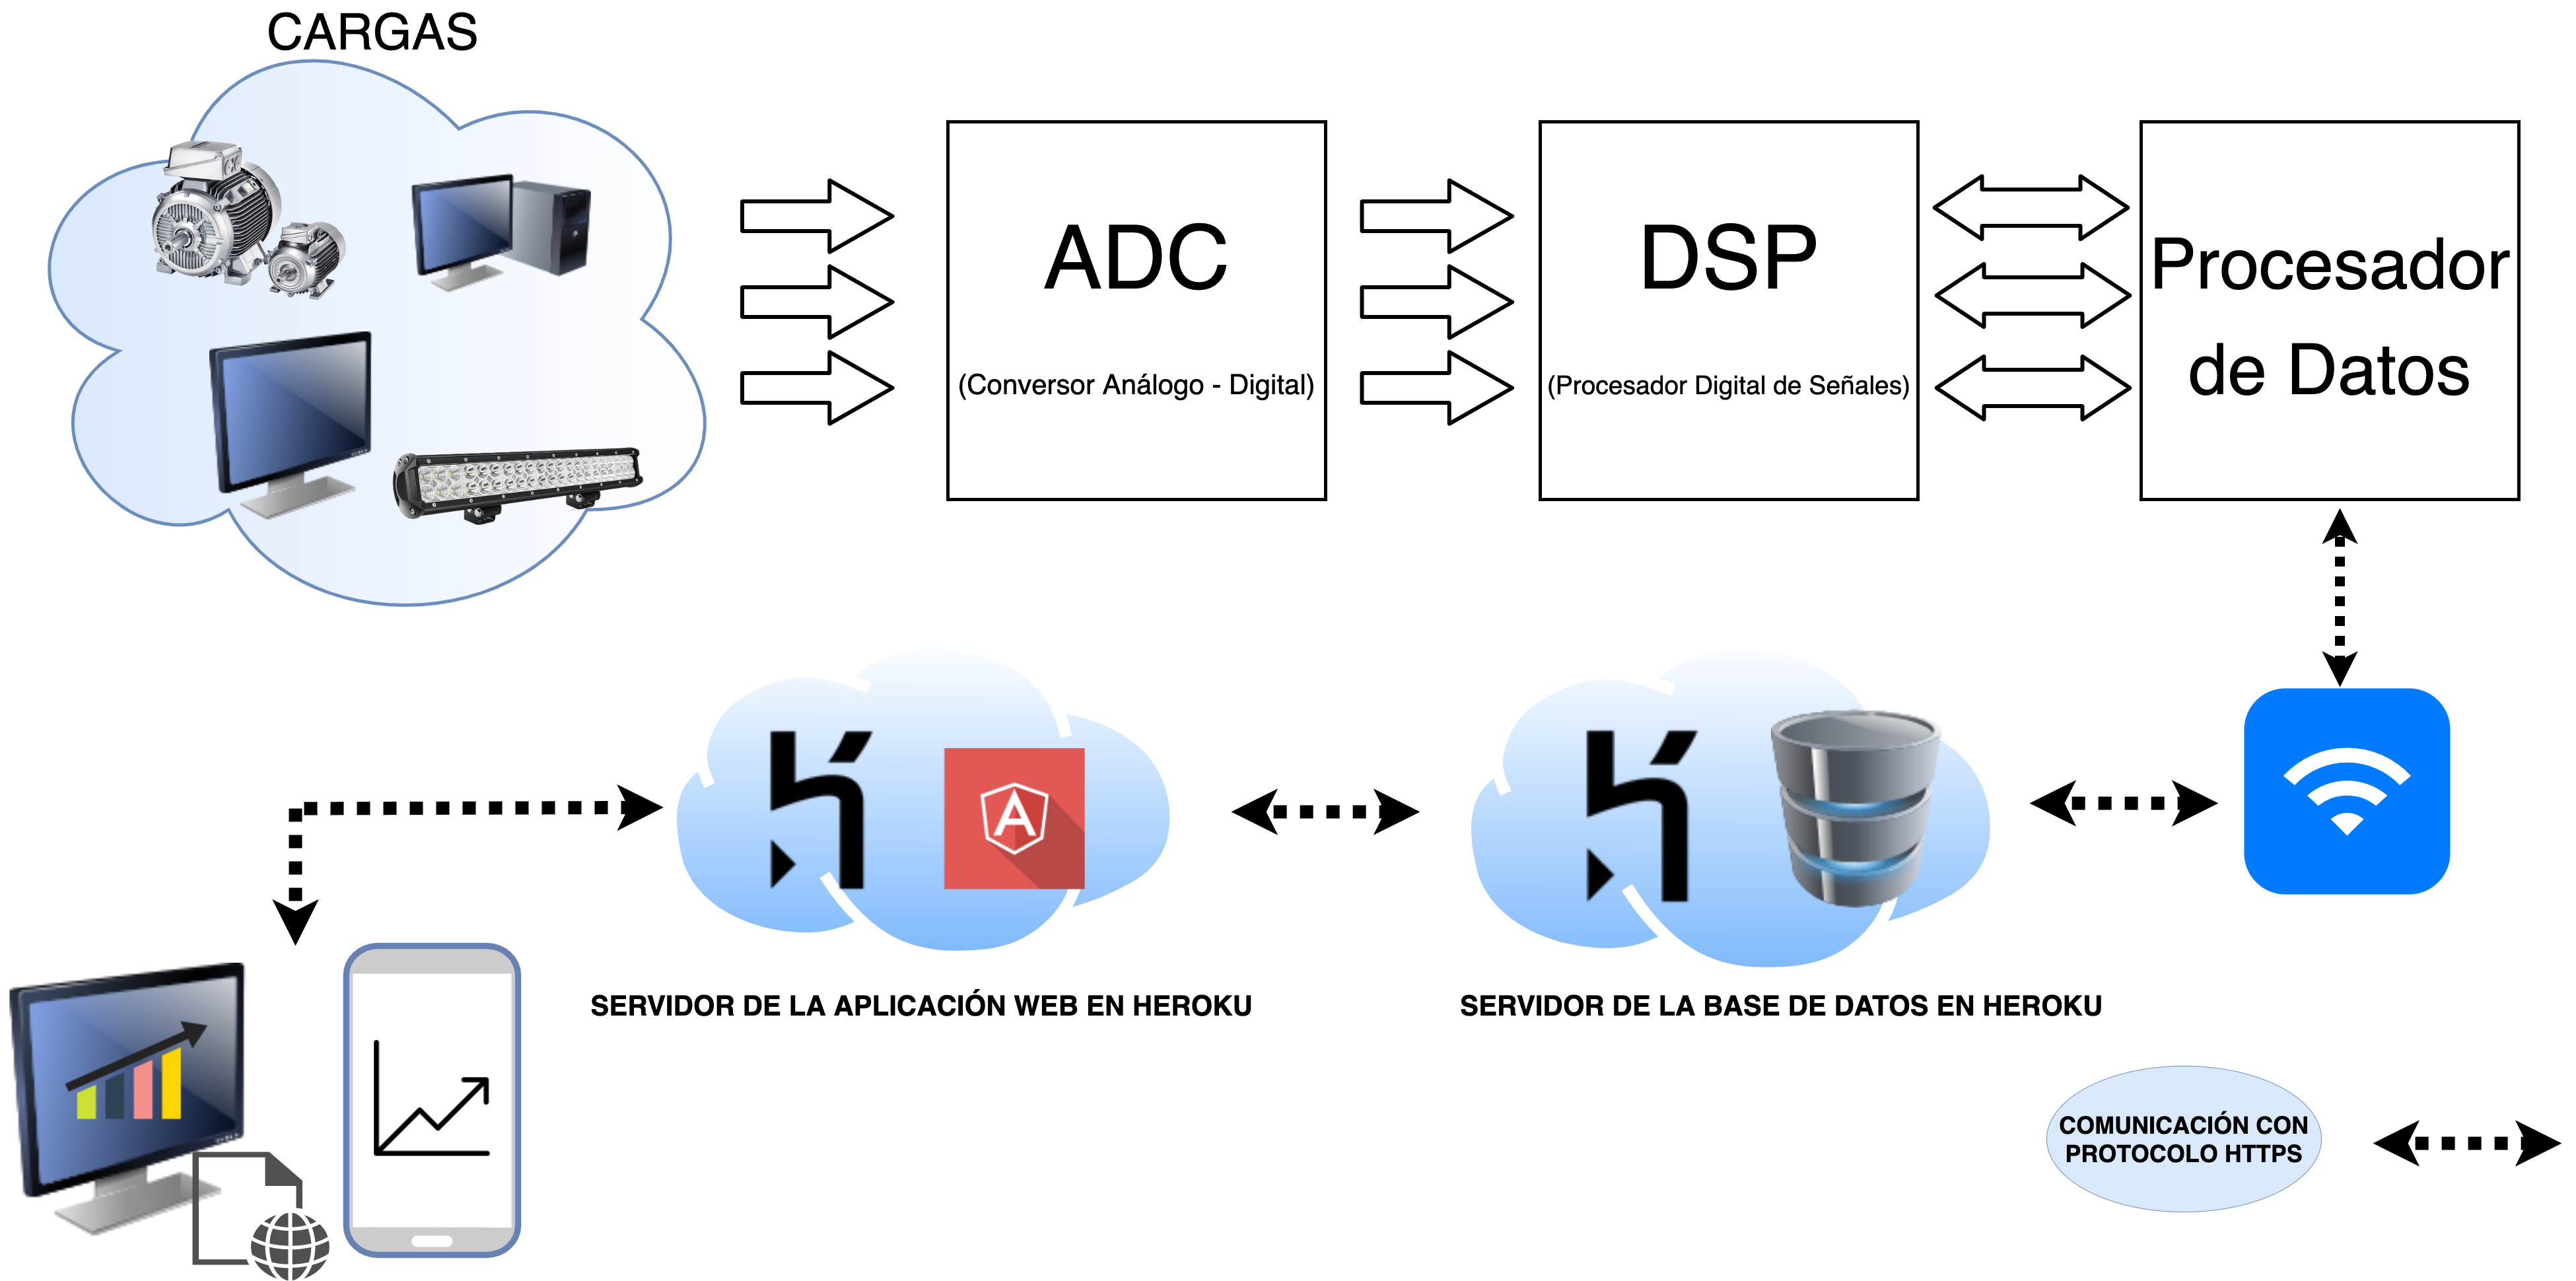
\includegraphics[width = 15cm]{3Proyecto/arquitectura}
\caption{Arquitectura del proyecto} 
\label{fig:arquitectura-proyecto}
\end{figure} 
En primera medida se planteó el diseño electrónico del medidor, iniciando por las cargas donde se conectan a un convertidor de señal análoga a digital, estas señales se pasan a un procesador digital de señales, dónde se aplica los parámetros matemáticos establecidos en el estándar IEEE 1459 del 2010, el cual da la medición de la potencia eléctrica en cualquier tipo de condición.\\\\
Dicho esto, la información se envía a un procesador de datos, este se encarga de administrar el manejo que se le da a los datos como lo es su lectura, escritura y filtración de los datos. El procesador debe contar con conexión a internet ya sea por wifi o ethernet con el fin de guardar la información en una base datos que está alojada en un servidor en la nube, la comunicación que tiene el procesador de datos con el servidor es por protocolo HTTPS.\\\\
Por lo tanto, el servidor en la nube que se planteó es Heroku ya que tiene la opción de una cuenta gratuita y así hostear la base de datos y la aplicación web sin ningún costo. Por ende las restricciones que tiene este plan, es que no se puede escoger el dominio de la página y hay un límite de espacio de 512MB pero es más que suficiente para el peso que tiene la base de datos de 21.5MB y la aplicación web de 65.2MB.\\\\
Una vez configurado el servidor, se escogió el framework javascript Angular 7 para el desarrollo de la aplicación web, ya que por medio del lenguaje de programación Typescript, el cual es un lenguaje tipado y robusto, nos permite tener mayor manipulación y consistencia en los datos; la aplicación utiliza una arquitectura RESTful y este permite, realizar peticiones HTTPS a la base de datos.\\\\
Finalmente, la información se visualiza de forma gráfica y númerica en una página web, en donde se pueden ver los valores de voltaje (V), corriente (A), potencia activa(W), potencia aparente (VA), potencia reactiva(VAR) y porcentaje de distorsión armónica en corriente y voltaje en cada fase.\\\\


\section{Fase de integración}
Considerando las fases y la magnitud del proyecto se decidió investigar e integrar un dispositivo que hiciera el análisis de las señales aplicando las ecuaciones del STD IEEE 1459 del 2010. Durante la búsqueda se encontró que los dispositivos más cercanos son los siguientes:\\
\begin{enumerate}
    \itemsep0em
    \item EVM430-F6779-3 Phase Electronic Watt-Hour EVM
    \item EVAL-ADE 7978
    \item 78M6631 3-Phase PowerMeasurement IC
\end{enumerate}

A continuación se detalla las tarjetas mencionadas:\\
\subsubsection{EVM430-F6779-3 Phase Electronic Watt-Hour EVM}
\begin{figure}
\centering
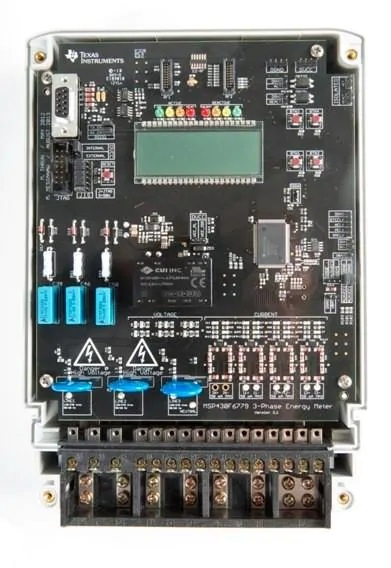
\includegraphics[width = 3cm]{3Proyecto/EVM430-F6779}
\caption{Tarjeta EVM430-F6779-3} 
\label{fig:EVM430-F6779-3}
\end{figure} 
\begin{itemize}
\itemsep0em
\item Es posible ejecutar aplicaciones de medición en tiempo real.
\item Viene con software de medición.
\item Se puede conectar a cualquier sistema de prueba o voltaje AC.
\item Fuentes de alimentación capacitaras y aisladas presentes
\item Fácil visualización de resultados y calibración a través de RS-232
\item Pantalla LCD de 160 segmentos
\item Conectores RF para soporte AMR / AMI
\item Soporte RTC de 32 kHz (cabecera disponible para calibración RTC)
\item Encabezados para alimentación MSP430 o solo  RTC a través de fuentes de alimentación auxiliares
\end{itemize}
\subsubsection{EVAL-ADE 7978}
\begin{figure}[H]
\centering
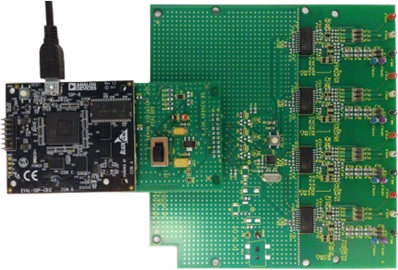
\includegraphics[width = 3cm]{3Proyecto/EVAL-ADE7978}
\caption{Tarjeta EVAL-ADE7978} 
\label{fig:EVAL-ADE7978}
\end{figure}
\begin{itemize}
\itemsep0em
\item Permite sensores Shunt en medidores de energía polifásica. 
\item Inmune a la manipulación magnética.
\item Alta precisión; admite EN 50470-1, EN 50470-3, IEC 62053-21, IEC 62053-22, IEC 62053-23, ANSI C12.20, y la estándar IEEE 1459.
\item Compatible con 3 fases, 3 o 4 lineas (Delta o estrella).
\item Calcula la energia Activa, Pasiva y Aparente en cada fase y en el sistema general.
\item Menos del 0.2\% de error en energía activa y reactiva en un rango dinámico de 2000 a 1 a TA = 25$^{\circ}$C
\item Menos del 0.1\% de error en voltaje rms en un rango dinámico de 500 a 1 a TA = 25$^{\circ}$C.
\item Menos del 0.25\% de error en corriente rms en un rango dinámico de 500 a 1 a TA = 25$^{\circ}$C.
\item Mediciones de calidad  de , incluida  la distorsión armónica total (THD).
\item Suministro de 3.3 V.
\item Temperatura de funcionamiento: -40$^{\circ}$C a +85$^{\circ}$C. 
\item Interfaces seriales flexibles I2C, SPI y HSDC.
\end{itemize}
\subsubsection{78M6631 3-Phase PowerMeasurement IC}
\begin{figure}[H]
\centering
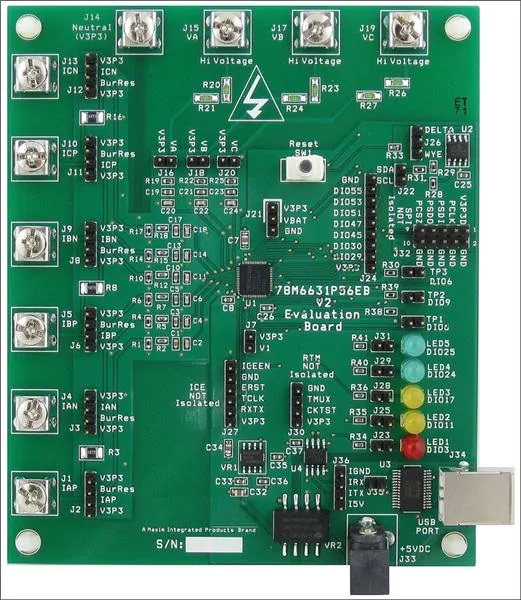
\includegraphics[width = 3cm]{3Proyecto/78M6631-EVM-DSL}
\caption{Tarjeta 78M6631-EVM-DSL}
\label{fig:78M6631-EVM-DSL}
\end{figure}
\begin{itemize}
\itemsep0em
\item 0.5 \% de precisión de vatios sobre 2000 : 1 corriente Rango y temperatura exclusiva
\item Excede los estándares IEC 62053 / ANSI C12.20.
\item Referencia de voltaje <40 ppm/ $^{\circ}$C.
\item Seis entradas analógicas que admiten entradas de medición de corriente y voltaje trifásico.
\item Configuración delta o estrella.
\item ADC Delta-Sigma de 22 bits con motor de cómputo (CE) independiente de 32 bits.
\item MPU de 8 bits (80515), un ciclo de reloj por instrucción con 4 KB MPU XRAM.
\item 128 KB Flash con seguridad.
\item Base de tiempo de 32 kHz con temporizador de vigilancia de hardware
\item Opciones de interfaz de host UART, I2C y High-Speed Slave SPI.
\item 17 pines I/O tolerante a 5V de uso general.
\end{itemize}

Teniendo encenta las características encontradas en las tres tarjetas, se decidió escoger el dispositivo ADE 7978 ya que cumple con la norma IEEE 1459 y tiene una medición precisa, ademas de esto la resolución del dispositivo es mucho mejor que el de los otros ( 24 bits ).
\section{Desarrollo del Hardware}
\subsection{Configuración inicial}

La conexión que se realizó, fue una configuración de 3 fases, 4 hilos, distribución estrella. El diagrama de conexión se ve en la figura \ref{fig:configuracion}

\begin{figure}[H]
    \begin{center}
    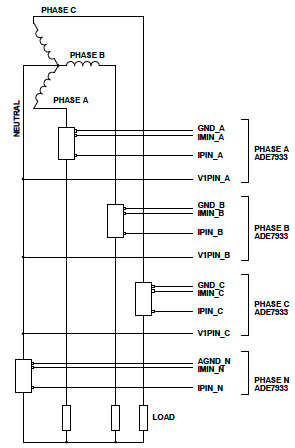
\includegraphics[width = 9cm]{3Proyecto/configuration}
    \caption{ Esquema de conexión para una distribución en Y, 3 fases, 4 hilos.} 
    \label{fig:configuracion}
    \end{center}
    \end{figure}

\subsubsection{Materiales}
\begin{itemize}
\itemsep0em
\item 4 resistencias Shunt.
\item 1m de cable 7 hilos 22 AWG azul - V1PIN.
\item 1m de cable 7 hilos 22 AWG cafe - GND.
\item 1m de cable 7 hilos 22 AWG amarillo - IMIN.
\item 1m de cable 7 hilos 22 AWG rojo - IPIN.
\item 2m de cable duplex 2x10 AWG blanco
\item 10 TYP UK2.50.
\item Carril de aluminio.
\item lamina de acetato.
\item 20 terminales.
\item 4 postes Met 10mm.
  
\end{itemize}

\begin{figure}[H]
\begin{center}
\includegraphics[width = 3cm]{3Proyecto/Cableado}
\caption{ ADE 7978 configurado con las resistencias Shunt} 
\label{fig:Cableado}
\end{center}
\end{figure}
Para configurar la tarjeta fue necesario encontrar una resistencia Shunt que se ajustará a las especificaciones del circuito a implementar, sin embargo este trabajo fue mas complicado, ya que las resistencias Shunt disponibles en el mercado son costosas y la mayoría de ellas vienen con resistencias bajas, elevando el voltaje de salida y ampliando el rango de medición del medidor ($\dfrac{I}{R}=V$), se decidió comprar 4 resistencias Shunt caseras las cuales tenían un costo de tan solo \$4.000 COP muy bajo comparado con las importadas o fabricadas industrial mente, en las que su valor esta entre \$50.000 COP - \$ 200.000 COP.\\
Teniendo todos los materiales, se realiza la conexión de la figura \ref{fig:configuracion}, utilizando el cable azul para el pin V1PIN, el cable café para el pin GND, el cable amarillo para el pin IMIN, el cable rojo para el pin IPIN y el cable blanco para conectar las shunt con el bloque de terminales, todo el montaje puesto sobre una lamina de acetato elevando la tarjeta con los 4 postes Met como se muestra en la figura \ref{fig:Cableado}\\

\subsection{Caracterización de la resistencia Shunt}
\begin{table} [H]
    \begin{center}
    \begin{tabular}{ |c|c|c|c|c|c|c|c|c| }
        \hline 
        Corriente (A) & 0.552 & 0.558 & 0.565 & 0.566 & 0.575 & 0.583 & 0.586 & 0.597\\
        \hline
        Voltaje (V) & 0.00105 & 0.00105 & 0.00107 & 0.00107 & 0.00107 & 0.00108 & 0.00109 & 0.00109\\
        \hline
        \hline 
        Corriente (A) & 0.609 & 0.621 & 0.639 & 0.651 & 0.68 & 0.7 & 0.73 & 0.757\\
        \hline
        Voltaje (V) & 0.00111 & 0.00113 & 0.00115 & 0.00117 & 0.0012 & 0.00122 & 0.00125 & 0.0013\\
        \hline
        \hline 
        Corriente (A) & 0.784 & 0.813 & 0.85 & 0.888 & 0.935 & 1.02 & 1.06 & 1.12\\
        \hline
        Voltaje (V) & 0.00134 & 0.00136 & 0.00143 & 0.00148 & 0.00153 & 0.00162 & 0.0017 & 0.00179\\
        \hline
        \hline 
        Corriente (A) & 1.21 & 1.28 & 1.38 & 1.45 & 1.59 & 1.63 & 1.75 & 1.8\\
        \hline
        Voltaje (V) & 0.0019 & 0.002 & 0.0022 & 0.00226 & 0.00246 & 0.00254 & 0.0027 & 0.00277\\
        \hline
        \hline 
        Corriente (A) & 1.75 & 1.67 & 1.5 & 1.42 & 1.35 & 1.24 & 1.18 & 1.1\\
        \hline
        Voltaje (V) & 0.00269 & 0.00257 & 0.00233 & 0.00222 & 0.00211 & 0.00196 & 0.00187 & 0.00176\\
        \hline
        \hline 
        Corriente (A) & 1.06 & 1.01 & 0.97 & 0.92 & 0.879 & 0.84 & 0.816 & 0.777\\
        \hline
        Voltaje (V) & 0.00169 & 0.00163 & 0.00158 & 0.00151 & 0.00145 & 0.0014 & 0.00137 & 0.00131\\
        \hline
        \hline 
        Corriente (A) & 0.753 & 0.734 & 0.71 & 0.693 & 0.67 & 0.652 & 0.629 & 0.616\\
        \hline
        Voltaje (V) & 0.00127 & 0.00125 & 0.00122 & 0.00119 & 0.00116 & 0.00115 & 0.00112 & 0.00111\\
        \hline
        \hline
        Corriente (A) & 0.605 & 0.591 & 0.575 & 0.562 & 0.555 \\
        \hline
        Voltaje (V) & 0.0011 & 0.00108 & 0.00107 & 0.00105 & 0.00104 \\ 
        \hline
    \end{tabular}
\end{center}
\caption{Corriente vs Voltaje en la resitencia shunt A}
\label{tab:shuntA}
\end{table}




\begin{table} [H]
    \begin{center}
    \begin{tabular}{ |c|c|c|c|c|c|c|c|c| }
        \hline
        Corriente (A) & 0.549 & 0.574 & 0.606 & 0.633 & 0.67 & 0.698 & 0.744 & 0.77\\
        \hline
        Voltaje (V) & 0.00107 & 0.00111 & 0.00112 & 0.00115 & 0.00119 & 0.00125 & 0.0013 & 0.00133\\
        \hline
        \hline
        Corriente (A) & 0.823 & 0.867 & 0.922 & 0.99 & 1.05 & 1.15 & 1.23 & 1.36\\
        \hline
        Voltaje (V) & 0.0014 & 0.00145 & 0.00152 & 0.0016 & 0.0017 & 0.00186 & 0.00196 & 0.00213\\
        \hline
        \hline
        Corriente (A) & 1.48 & 1.69 & 1.8 & 1.7 & 1.48 & 1.35 & 1.22 & 1.15\\
        \hline
        Voltaje (V) & 0.0023 & 0.0026 & 0.00278 & 0.00262 & 0.0023 & 0.00214 & 0.00194 & 0.00182\\
        \hline
        \hline
        Corriente (A) & 1.05 & 0.977 & 0.913 & 0.85 & 0.811 & 0.76 & 0.728 & 0.685\\
        \hline
        Voltaje (V) & 0.0017 & 0.00162 & 0.00151 & 0.00143 & 0.00139 & 0.00132 & 0.00127 & 0.0012\\
        \hline
        \hline
        Corriente (A) & 0.662 & 0.635 & 0.611 & 0.599 & 0.58 & 0.557\\
        \hline
        Voltaje (V) & 0.00119 & 0.00116 & 0.00113 & 0.0011 & 0.00109 & 0.00108\\
        \hline
    \end{tabular}
\end{center}
\caption{Corriente vs Voltaje en la resitencia shunt B}
\label{tab:shuntB}
\end{table}


\begin{table} [H]
    \begin{center}
    \begin{tabular}{ |c|c|c|c|c|c|c|c|c| }
        \hline
        Corriente (A) & 0.557 & 0.573 & 0.593 & 0.631 & 0.654 & 0.69 & 0.717 & 0.752\\
        \hline
        Voltaje (V) & 0.00106 & 0.00108 & 0.0011 & 0.00115 & 0.00117 & 0.00122 & 0.00126 & 0.00131\\
        \hline
        \hline
        Corriente (A) & 0.8 & 0.838 & 0.896 & 0.95 & 1.03 & 1.09 & 1.19 & 1.29\\
        \hline
        Voltaje (V) & 0.00137 & 0.00141 & 0.00149 & 0.00155 & 0.00166 & 0.00175 & 0.00189 & 0.00205\\
        \hline
        \hline
        Corriente (A) & 1.47 & 1.59 & 1.8 & 1.63 & 1.52 & 1.37 & 1.27 & 1.15\\
        \hline
        Voltaje (V) & 0.0023 & 0.00246 & 0.00276 & 0.00251 & 0.00237 & 0.00215 & 0.00199 & 0.00183\\
        \hline
        \hline
        Corriente (A) & 1.07 & 0.98 & 0.925 & 0.86 & 0.816 & 0.766 & 0.737 & 0.697\\
        \hline
        Voltaje (V) & 0.00172 & 0.0016 & 0.00153 & 0.00144 & 0.00138 & 0.00131 & 0.0013 & 0.00121\\
        \hline
        \hline
        Corriente (A) & 0.661 & 0.633 & 0.616 & 0.599 & 0.558\\
        \hline
        Voltaje (V) & 0.00119 & 0.00115 & 0.00113 & 0.00111 & 0.00107\\
        \hline
    \end{tabular}
\end{center}
\caption{Corriente vs Voltaje en la resitencia shunt C}
\label{tab:shuntC}
\end{table}
\subsection{Conversión de voltaje}
Para obtener el voltaje de entrada del ADE7978, se realizaron los siguientes pasos:\\

La carga se conecta a la fase siguiendo el diagrama de conexión \ref{fig:configuracion}. Los pines V1PIN y GND\_A, pasan por un divisor de voltaje donde su salida es el pin V1P y VM como se ve en la figura \ref{fig:divisorVolate}. El divisor se modela bajo la siguiente ecuación:\\

\begin{equation}
    V1P = \frac{R_{2}}{R_{1} + R_{2}} * V_{in}
\end{equation}

Donde $\; R1 = 990150 \ohm$, \;$R2 = 1 K\ohm$.\\

\begin{equation}\label{divisorVoltaje}
    V1P = 0.00100893 * V_{in}
\end{equation}

El divisor de voltaje es necesario ya que el conversor ADE7933 solo debe recibir valores en un rango de $\pm 0.5V$. 

El voltaje VA es la diferencia de voltaje que hay entre V1P y VM, esta es la señal que el conversor transforma a digital. La salida digital que entrega el conversor tiene un rango de $\pm 5.320.000$ como se ve en la figura \ref{fig:voltageOutput}. Esta señal entra al ADE7978 y de ahí en adelante, todos los procesos que se ejecutan, son basados en la conversión anteriormente descrita.\\

La relación de entrada y salida del conversor ADE7933, consiste en un voltaje pico de entrada de $0.5 V$, genera una señal de salida de $5.320.000$.\\

La siguiente ecuación relaciona la señal de salida del conversor con la señal de entrada al medidor:\\

\begin{align*}
    &0,5V \rightarrow 5,320,000.\\
    &V1P \rightarrow DRV
\end{align*}

Donde $DRV = Dato\;del\;rango\;de\;voltaje\;del\;conversor$\\

\begin{equation}
    V1P = \frac{DRV * 0.5}{5.320.000}
\end{equation}

\begin{equation}\label{relacionConversor}
    V1P = DRV * 9,39845 * 10^{-8} 
\end{equation}

Reemplazando la ecuación del divisor de voltaje \ref{divisorVoltaje} en \ref{relacionConversor}

\begin{align*}
    0.00100893 * V_{in} = DRV * 9,39845 * 10^{-8} 
\end{align*}

\begin{equation}\label{conversorEntradaSalida}
    V_{in} = DRV * 0,00009315311
\end{equation}
La ecuación \ref{conversorEntradaSalida} modela la relación del voltaje de entrada al circuito al rango de voltaje del conversor.

\begin{figure}[H]
    \centering
    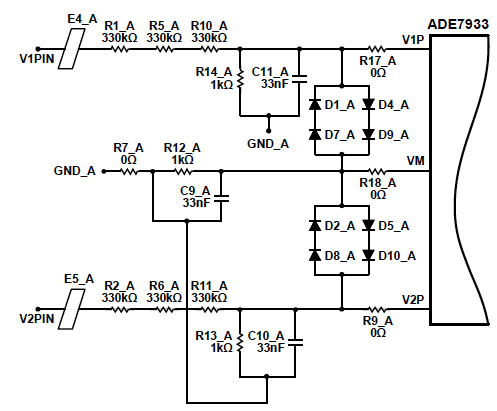
\includegraphics[width = 10cm]{3Proyecto/divisorVoltaje}
    \caption{Divisor de voltaje ADC} 
    \label{fig:divisorVolate}
\end{figure} 

\begin{figure}[H]
    \centering
    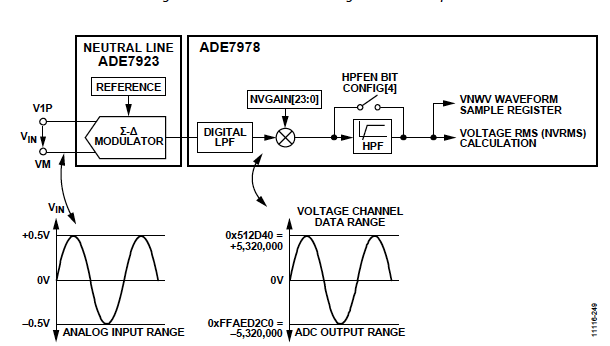
\includegraphics[width = 10cm]{3Proyecto/voltageOutput}
    \caption{Salida de voltaje del ADE 7978} 
    \label{fig:voltageOutput}
\end{figure} 


\subsection{Conversión de corriente}
Para encontrar la relación que hay entre la entrada de corriente y el convertidor ADC fue necesario utilizar la ecuación de la recta arrojada por las muestras de la caracterización de las shunt y también fue necesario hallar la relación de voltaje entre el pin IP e IM que son los usados por el ADC figura \ref{fig:CircuitoCorriente}


\begin{figure}[H]
    \begin{center}
        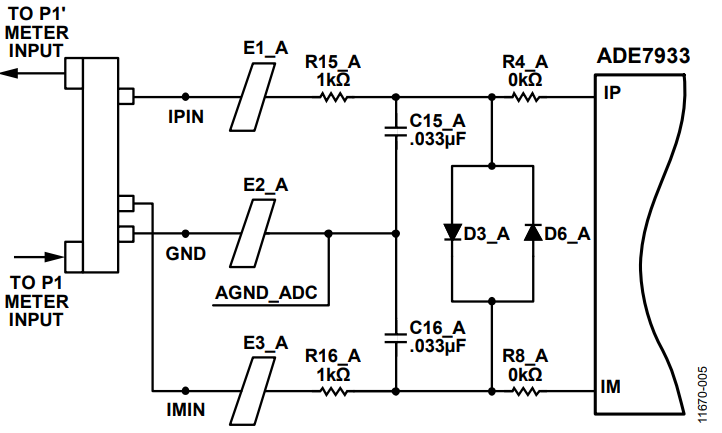
\includegraphics[width = 10cm]{3Proyecto/CircuitoCorriente.PNG}
    \caption{ Circuito de protección para los pines IP e IM } 
    \label{fig:CircuitoCorriente}
   \end{center}
\end{figure}

Como ya se tiene la relación entre la corriente de entrada y el voltaje de salida en la Shunt se procede hallar el voltaje entre el pin IP e IM resolviendo el circuito por medio del teorema de nodos como se muestra en la figura \ref{fig:Nodos}
\begin{figure}[H]
    \begin{center}
        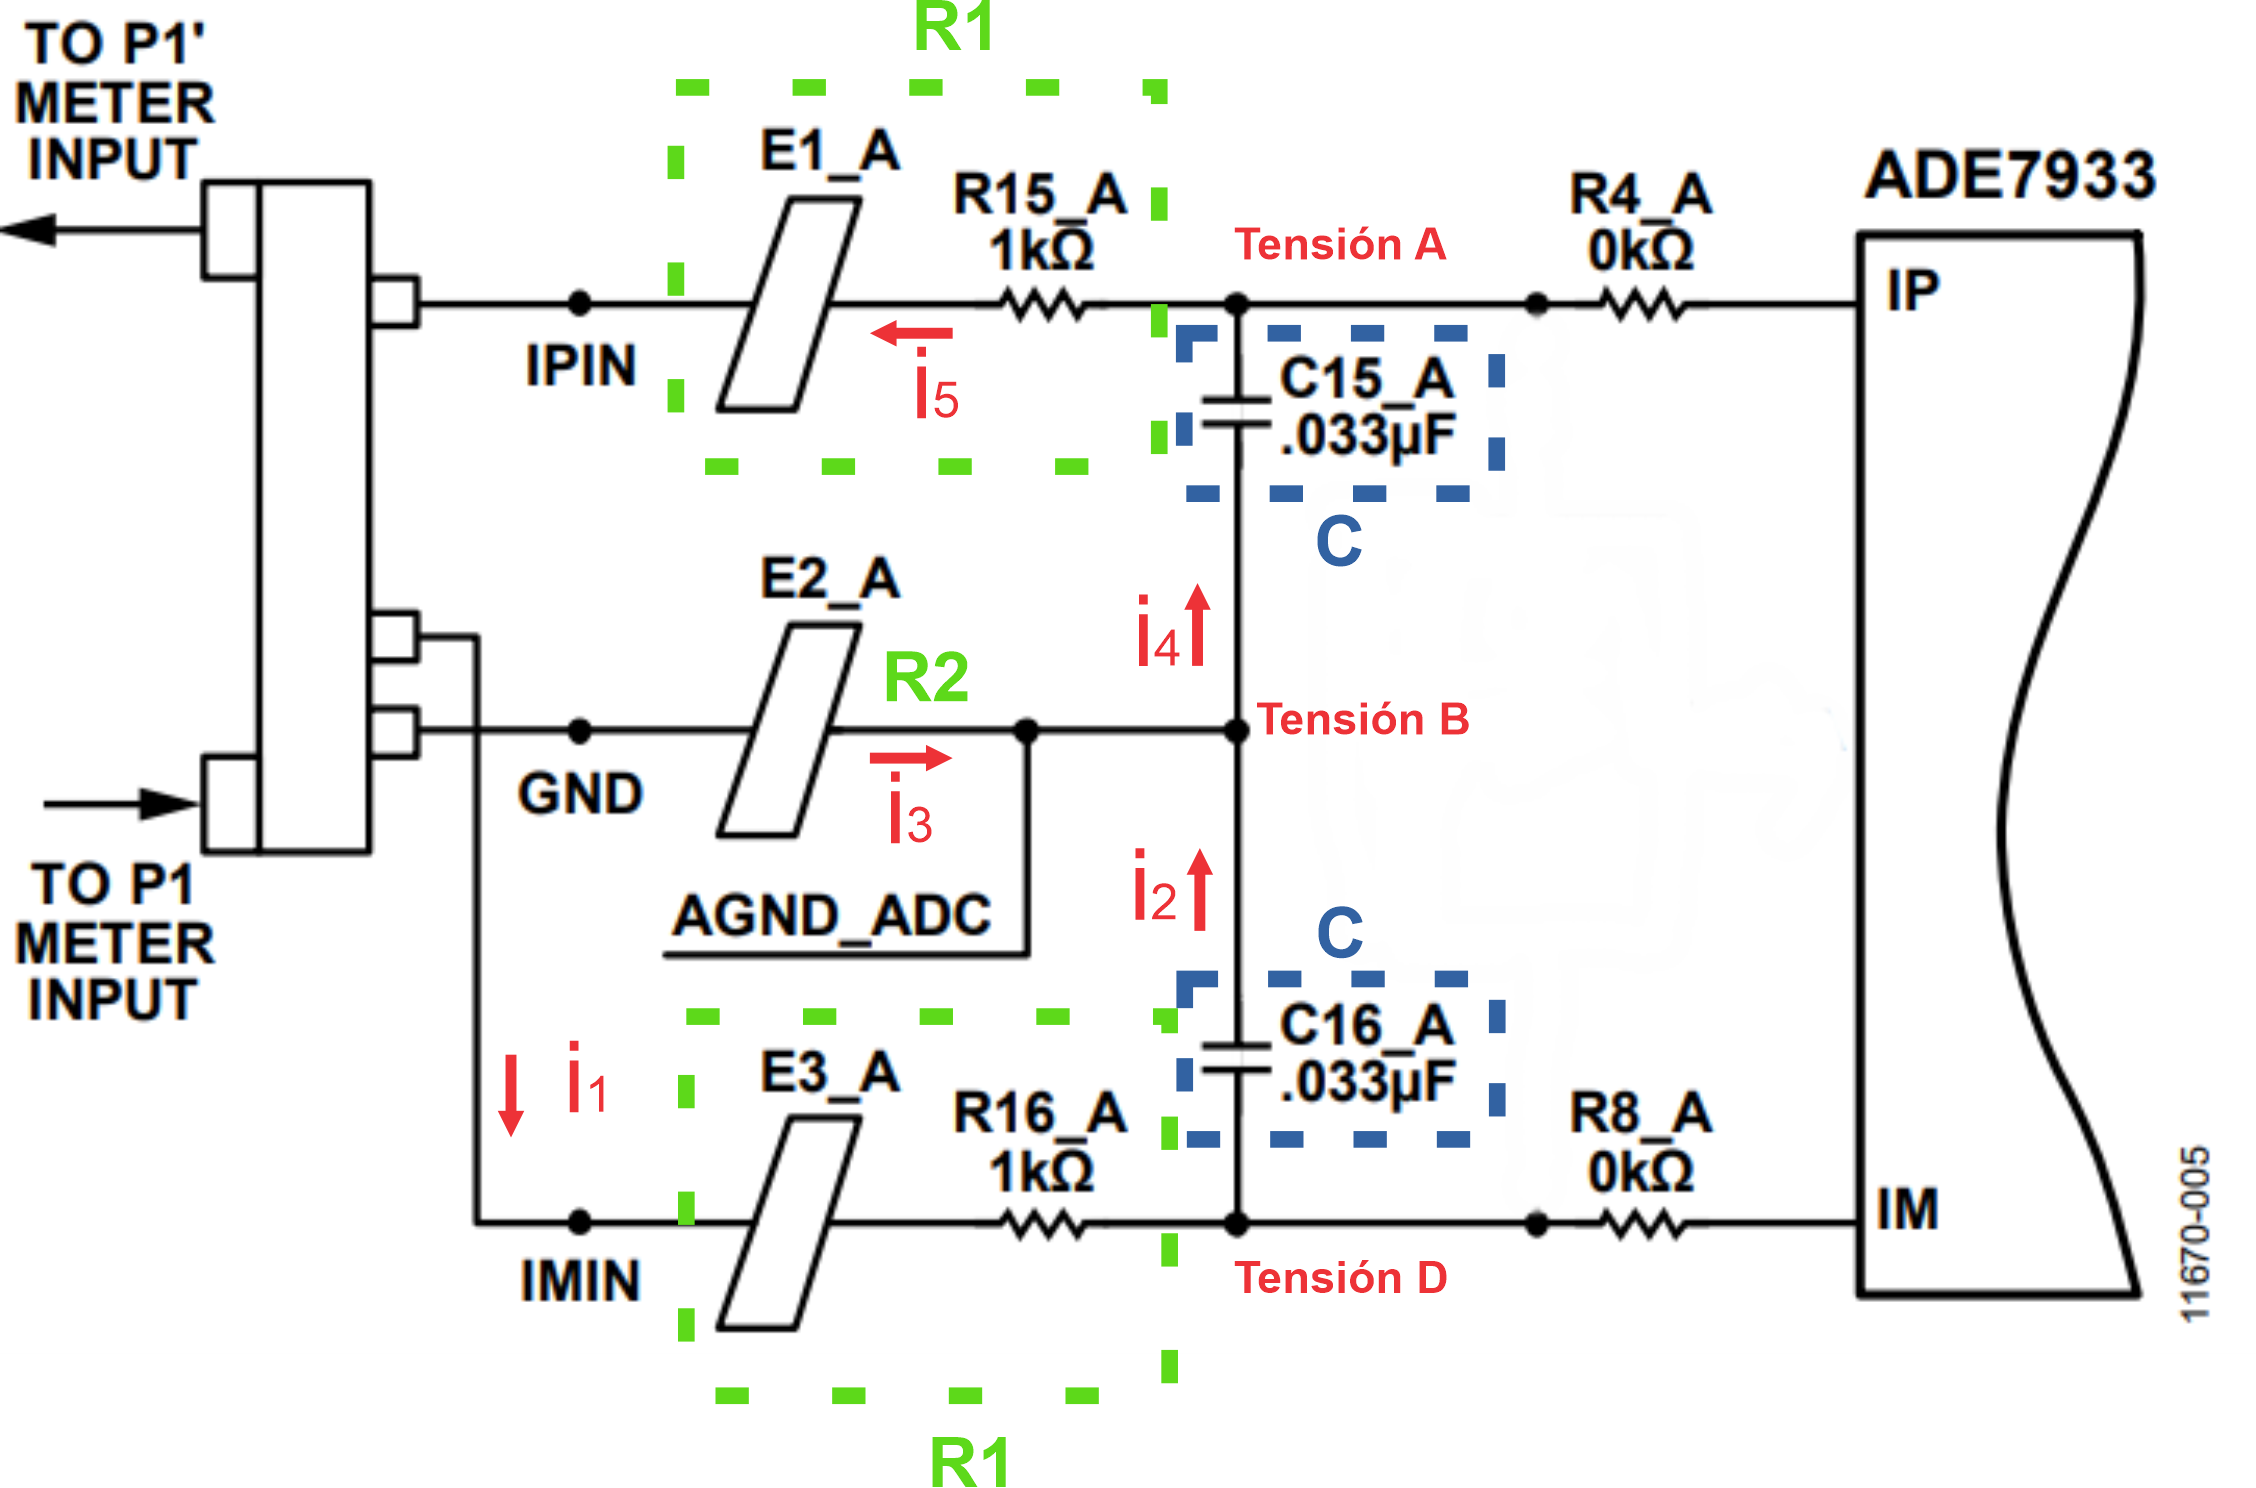
\includegraphics[width = 10cm]{3Proyecto/Nodos.PNG}
    \caption{ Nodos aplicados al circuito} 
    \label{fig:Nodos}
   \end{center}
\end{figure}

Se asume que el circuito se alimenta con una fuente de voltaje AC con terminal $+$ en IPIN y terminal $-$ en GND e IMIN resolviendo de la siguiente manera :
\\  
\begin{equation}\label{Nodo D}
\end{equation}

Con las ecuaciones obtenidas de cada nodo se despeja cada una de ellas dejándola igualada a una variable 
\begin{itemize}
    \item \textbf{Nodo A} \\
    $\mathbf{i_{1}=i_{2}}$
    \begin{align*}
        \frac{V_{i}}{R_{1}} - \frac{A}{R_{1}} = \frac{A}{ZC} - \frac{B}{ZC} \\\\
        \frac{V_{i}}{R_{1}} = A(\frac{1}{R_{1}}+\frac{1}{ZC}) -\frac{B}{ZC} \\\\
        \frac{V_{i}}{R_{1}} = A\frac{R_{1}+ZC}{R_{1}ZC} -\frac{B}{ZC} \\\\
            \frac{B}{ZC} = A\frac{R_{1}+ZC}{R_{1}ZC} - \frac{V_{i}}{R_{1}}
        \end{align*}
        \begin{equation}\label{Nodo A}
            B = A\frac{R_{1}+ZC}{R_{1}} - V_{i}\frac{ZC}{R_{1}}
        \end{equation}
        \item \textbf{Nodo B} \\
        $ \mathbf{i_{2}=i_{3}+i_{4}}$
        \begin{align*}
            \frac{A}{ZC} - \frac{B}{ZC} = \frac{B}{R_{2}} + \frac{B}{ZC} - \frac{D}{ZC} \\\\
            \frac{A}{ZC} + \frac{D}{ZC} = B(\frac{1}{R_{2}} + \frac{1}{ZC} + \frac{1}{ZC}) \\\\
            \frac{A}{ZC} + \frac{D}{ZC} = B(\frac{1}{R_{2}} + \frac{2}{ZC} ) \\\\
            \frac{A}{ZC} + \frac{D}{ZC} = B\frac{2R_{2}+ZC}{R_{2}ZC} 
        \end{align*}
        \begin{equation}\label{Nodo B}
            B = A\frac{R_{2}}{2R_{2}+ZC} + D\frac{R_{2}}{2R_{2}+ZC}
        \end{equation}
        \item \textbf{Nodo D} \\
        $ \mathbf{i_{4}=i_{5}}$
        \begin{align*}
            \frac{B}{ZC} - \frac{D}{ZC} = \frac{D}{R_{3}} \\\\
            \frac{B}{ZC} = D(\frac{1}{R_{3}} + \frac{1}{ZC}) \\\\
            \frac{B}{ZC} = D\frac{R_{3}+ZC}{R_{3}ZC}
        \end{align*}
        \begin{equation}\label{Nodo D}
            B = D\frac{R_{3}+ZC}{R_{3}} 
        \end{equation}
    \end{itemize}
    
    Remplazando la ecuación \ref{Nodo B} en la ecuación \ref{Nodo A}
    \begin{align*}
        A\frac{R_{2}}{2R_{2}+ZC} + D\frac{R_{2}}{2R_{2}+ZC} = A\frac{R_{1}+ZC}{R_{1}} - V_{i}\frac{ZC}{R_{1}} \\\\
        D\frac{R_{2}}{2R_{2}+ZC} = A(\frac{R_{1}+ZC}{R_{1}} - \frac{R_{2}}{2R_{2}+ZC})- V_{i}\frac{ZC}{R_{1}} \\\\
        D\frac{R_{2}}{2R_{2}+ZC} = A\frac{(R_{1}+ZC)(2R_{2}+ZC) - R_{1}R_{2}}{R_{1}(2R_{2}+ZC)} - V_{i}\frac{ZC}{R_{1}} \\\\
        D = A\frac{((R_{1}+ZC)(2R_{2}+ZC) - R_{1}R_{2})(2R_{2}+ZC)}{R_{1}R_{2}(2R_{2}+ZC)} - V_{i}\frac{ZC(2R_{2}+ZC)}{R_{1}R_{2}}
    \end{align*}
    \begin{equation}\label{Nodo B en A}
        D = A\frac{(R_{1}+ZC)(2R_{2}+ZC) - R_{1}R_{2}}{R_{1}R_{2}} - V_{i}\frac{ZC(2R_{2}+ZC)}{R_{1}R_{2}}
    \end{equation}
    
    Remplazando la ecuación \ref{Nodo B} en la ecuación \ref{Nodo D}
    \begin{align*}
        A\frac{R_{2}}{2R_{2}+ZC} + D\frac{R_{2}}{2R_{2}+ZC} = D\frac{R_{3}+ZC}{R_{3}} \\\\
        A\frac{R_{2}}{2R_{2}+ZC} = D(\frac{R_{3}+ZC}{R_{3}}-\frac{R_{2}}{2R_{2}+ZC}) \\\\
        A\frac{R_{2}}{2R_{2}+ZC} = D(\frac{(2R_{2}+ZC)(R_{3}+ZC)-R_{2}R_{3}}{R_{3}(2R_{2}+ZC)} \\\\
        AR_{2} = D(\frac{(2R_{2}+ZC)(R_{3}+ZC)-R_{2}R_{3}}{R_{3}}
    \end{align*}
    \begin{equation}\label{Nodo B en D}
        A\frac{R_{2}R_{3}}{(2R_{2}+ZC)(R_{3}+ZC)-R_{2}R_{3}} = D 
    \end{equation}
    
    Remplazando la ecuación \ref{Nodo B en D} en la ecuación \ref{Nodo B en A}
    \begin{align*}
        A\frac{R_{2}R_{3}}{(2R_{2}+ZC)(R_{3}+ZC)-R_{2}R_{3}} = A\frac{(R_{1}+ZC)(2R_{2}+ZC) - R_{1}R_{2}}{R_{1}R_{2}} - V_{i}\frac{ZC(2R_{2}+ZC)}{R_{1}R_{2}}\\\\ 
        V_{i}\frac{ZC(2R_{2}+ZC)}{R_{1}R_{2}} = A\frac{(R_{1}+ZC)(2R_{2}+ZC) - R_{1}R_{2}}{R_{1}R_{2}} - A\frac{R_{2}R_{3}}{(2R_{2}+ZC)(R_{3}+ZC)-R_{2}R_{3}} \\\\ 
        V_{i}\frac{ZC(2R_{2}+ZC)}{R_{1}R_{2}} = A(\frac{(R_{1}+ZC)(2R_{2}+ZC) - R_{1}R_{2}}{R_{1}R_{2}} - \frac{R_{2}R_{3}}{(2R_{2}+ZC)(R_{3}+ZC)-R_{2}R_{3}}) \\\\ 
        V_{i}\frac{ZC(2R_{2}+ZC)}{R_{1}R_{2}} = A\frac{ [(R_{1}+ZC)(2R_{2}+ZC) - R_{1}R_{2}] [(2R_{2}+ZC)(R_{3}+ZC) - R_{2}R_{3}] - R_{1}R_{2}^{2}R_{3}}{(R_{1}R_{2})((2R_{2}+ZC)(R_{3}+ZC)-R_{2}R_{3})} \\\\ 
        V_{i}ZC(2R_{2}+ZC) = A\frac{ [(R_{1}+ZC)(2R_{2}+ZC) - R_{1}R_{2}] [(2R_{2}+ZC)(R_{3}+ZC)-R_{2}R_{3}] - R_{1}R_{2}^{2}R_{3} }{ (2R_{2}+ZC)(R_{3}+ZC)-R_{2}R_{3} } \\\\ 
        V_{i}\frac{ [ZC(2R_{2}+ZC)] [(2R_{2}+ZC)(R_{3}+ZC)-R_{2}R_{3}] }{ [(R_{1}+ZC)(2R_{2}+ZC) - R_{1}R_{2}] [(2R_{2}+ZC)(R_{3}+ZC)-R_{2}R_{3}]-R_{1}R_{2}^{2}R_{3} } = A\\\\ 
    \end{align*}
    Con ayuda del software Matlab se simplifica la expresión remplazando los valores de cada elemento como se muestra en el datasheet
    \\
    $ R_{1} = 1150 \ohm;$ $R_{2} = 150 \ohm;$ $R_{3} = 1150 \ohm;$ $ZC = \frac{-j}{WC};$
    $W = 2 \pi f;$ $f = 60 Hz;$ $C = 0.033\mu f ;$
    \begin{equation}\label{final A}
        V_{i}(0.9998 - 0.0143j)=A
    \end{equation}
    Magnitud = 0.9999 \\
    Angulo = -0.0143 $^{\circ}$ \\
    Remplazando la ecuación \ref{final A} en la ecuación \ref{Nodo B en A} para encontrar el valor del nodo D
    \begin{align*}
        D = A\frac{(R_{1}+ZC)(2R_{2}+ZC) - R_{1}R_{2}}{R_{1}R_{2}} - V_{i}\frac{ZC(2R_{2}+ZC)}{R_{1}R_{2}}\\\\
        D = [V_{i}(0.9998 - 0.0143j)] [\frac{(R_{1}+ZC)(2R_{2}+ZC) - R_{1}R_{2}}{R_{1}R_{2}}] - V_{i}\frac{ZC(2R_{2}+ZC)}{R_{1}R_{2}}\\\\
        D = [V_{i}(0.9998 - 0.0143j)] [-3.7455e^{4} - 6.7567e^{2}j] - V_{i}(-3.7456e^{4} - 1.3979e^{2}j)\\\\
        D = V_{i} (-2.6677e^{-5} + 8.6311e^{-7}j) \\\\
    \end{align*}
    
    La relación que hay entre el pin IP e IM es la resta entre el nodo A y e nodo D
    
    \begin{align*}
        A-D = IP-IM\\\\
        V_{i}(0.9998 - 0.0143j) - V_{i} (-2.6677e^{-5} + 8.6311e^{-7}j) = IP-IM\\\\
        V_{i}(0.9998 - 0.0143j) = IP-IM \\
        V_{i} (0.9999 \angle -0.0143) =  IP-IM
    \end{align*}
    Usando la relación arrojada en la caracterización de las resistencias, se remplaza en esta ecuación para dejar la expresión en términos de corriente de entrada en la Shunt y voltaje entre el pin IP e IM\\\\
    \begin{align*}
        &1.38e^{-3} I + 2.56e^{-4} = V_{i}\\\\
    \end{align*}
    \begin{equation}\label{Relacion corriente}
        (1.38e^{-3} I + 2.56e^{-4})(0.9999 \angle -0.0143)  = IP-IM
    \end{equation}
    La siguiente ecuación relaciona la señal de salida del conversor con la señal de entrada al medidor:\\

    \begin{align*}
        &0.03125V \rightarrow 5,320,000.\\
        &IP-IM \rightarrow DRI
    \end{align*}
    
    Donde $DRI = Dato\;del\;rango\;de\;corriente\;del\;conversor$\\
    
    \begin{equation}\label{Relacion DRI}
        IP-IM = \frac{DRI * 0.03125}{5.320.000}
    \end{equation}
    
    Remplazando la ecuación \ref{Relacion corriente} en la ecuación \ref{Relacion DRI}
    \begin{align*}
        (1.38e^{-3} I + 2.56e^{-4})(0.9998 - 0.0143j) = \frac{DRI * 0.03125}{5.320.000} \\\\
        (0.0014 - 0.0000j)I + (2.5595e^{-4} - 3.6618e^{-6}j)  = \frac{DRI * 0.03125}{5.320.000} \\\\
        I = \frac{\frac{DRI * 0.03125}{5.320.000} - (2.5595e^{-4} - 3.6618e^{-6}j)}{(0.0014 - 0.0000j)}  \\\\
        I = DRI (4.2566e^{-6} + 6.0898e^{-8}j) - (0.1855 - 0.0000j)   \\\\
        I = 4.2570e^{-6}DRI  - 0.1855   \\\\
    \end{align*}
%\newpage{\clearpage}
\chapter{Resultados del proyecto}

\section{Primer Prueba}

Se procedió a realizar la primer prueba con nuestro medidor y debido que en ese momento el mundo se encontrabá en la pandemia del COVID-19, tocó realizar pruebas con cargas domésticas las culaes fueron las siguientes:
\begin{itemize}
    \itemsep0em
    \item Bombillo de 9 W.
    \item Portatil dell.
    \item Osciloscopio.
    \item Raspberry.
    \item TV de 111 W.
    \item Play Station 3,
    \item Parlantes.
    \item Licuadora.
    \item Licuadora Nutribullet.
    \item Plancha de 1000 W.
\end{itemize}
\begin{table}
    \caption{Resultados de la prueba Nº 1}
      \begin{tabular}{|l|r|r|r|}
      \toprule
      \multicolumn{1}{|c|}{\multirow{2}[4]{*}{CARGA}} & \multicolumn{1}{c|}{MULTÍMETRO} & \multicolumn{2}{c|}{TARJETA} \\
  \cmidrule{2-4}          & \multicolumn{1}{l|}{Corriente} & \multicolumn{1}{l|}{Voltaje} & \multicolumn{1}{l|}{Corriente} \\
      \midrule
      Bombillo led de 9WT & 0,0772 & 122   & 0,84175682 \\
      \midrule
      Portatil, osciloscopio, Raspberry, TV(111W), Play 3, Parlantes & 1,4   & 122   & 2,48453856 \\
      \midrule
      Licuadora & 2,11  & 122   & 3,10783076 \\
      \midrule
      Licuadora pequeña & 1,46  & 122   & 2,32913756 \\
      \midrule
      Licuadora + licuadora pequeña & 3,87  & 121   & 5,06727028 \\
      \midrule
      Plancha de 1000W & 9,2   & 118   & 10,7248316 \\
      \midrule
      Licuadora + licuadora pequeña + plancha & 12,55 & 116   & 14,6785336 \\
      \bottomrule
      \end{tabular}%
    \label{tab:resultado1-1}%
  \end{table}%
  

  \begin{table}[htbp]
    \centering
      \begin{tabular}{|c|c|r|r|r|r|}
      \toprule
      \multicolumn{2}{|c|}{OSCILOSCOPIO} & \multicolumn{2}{c|}{\cellcolor[rgb]{ .557,  .663,  .859}Diferencias de corriente (A)} & \multicolumn{2}{c|}{\cellcolor[rgb]{ .557,  .663,  .859}Diferencia de voltaje(V)} \\
      \midrule
      \multicolumn{2}{|c|}{Voltaje} & \multicolumn{1}{c|}{\cellcolor[rgb]{ .557,  .663,  .859}Error Absoluto} & \multicolumn{1}{c|}{\cellcolor[rgb]{ .557,  .663,  .859}Error relativo} & \multicolumn{1}{c|}{\cellcolor[rgb]{ .557,  .663,  .859}Error Absoluto} & \multicolumn{1}{c|}{\cellcolor[rgb]{ .557,  .663,  .859}Error relativo} \\
      \midrule
      \multicolumn{2}{|c|}{119,93} & \cellcolor[rgb]{ .557,  .663,  .859}0,764556821 & \cellcolor[rgb]{ .557,  .663,  .859}990\% & \cellcolor[rgb]{ .557,  .663,  .859}2,07 & \cellcolor[rgb]{ .557,  .663,  .859}2\% \\
      \midrule
      \multicolumn{2}{|c|}{119,53} & \cellcolor[rgb]{ .557,  .663,  .859}1,084538555 & \cellcolor[rgb]{ .557,  .663,  .859}77\% & \cellcolor[rgb]{ .557,  .663,  .859}2,47 & \cellcolor[rgb]{ .557,  .663,  .859}2\% \\
      \midrule
      \multicolumn{2}{|c|}{119,63} & \cellcolor[rgb]{ .557,  .663,  .859}0,997830763 & \cellcolor[rgb]{ .557,  .663,  .859}47\% & \cellcolor[rgb]{ .557,  .663,  .859}2,37 & \cellcolor[rgb]{ .557,  .663,  .859}2\% \\
      \midrule
      \multicolumn{2}{|c|}{119,87} & \cellcolor[rgb]{ .557,  .663,  .859}0,869137564 & \cellcolor[rgb]{ .557,  .663,  .859}60\% & \cellcolor[rgb]{ .557,  .663,  .859}2,13 & \cellcolor[rgb]{ .557,  .663,  .859}2\% \\
      \midrule
      \multicolumn{2}{|c|}{118,56} & \cellcolor[rgb]{ .557,  .663,  .859}1,197270279 & \cellcolor[rgb]{ .557,  .663,  .859}31\% & \cellcolor[rgb]{ .557,  .663,  .859}2,44 & \cellcolor[rgb]{ .557,  .663,  .859}2\% \\
      \midrule
      \multicolumn{2}{|c|}{120} & \cellcolor[rgb]{ .557,  .663,  .859}1,524831581 & \cellcolor[rgb]{ .557,  .663,  .859}17\% & \cellcolor[rgb]{ .557,  .663,  .859}-2 & \cellcolor[rgb]{ .557,  .663,  .859}2\% \\
      \midrule
      \multicolumn{2}{|c|}{114,5} & \cellcolor[rgb]{ .557,  .663,  .859}2,128533554 & \cellcolor[rgb]{ .557,  .663,  .859}17\% & \cellcolor[rgb]{ .557,  .663,  .859}1,5 & \cellcolor[rgb]{ .557,  .663,  .859}1\% \\
      \midrule
      \multicolumn{2}{|c|}{**Promedio de diferencia =} & \cellcolor[rgb]{ .557,  .663,  .859}1,22381416 & \cellcolor[rgb]{ .557,  .663,  .859}177\% & \cellcolor[rgb]{ .557,  .663,  .859}1,568571429 & \cellcolor[rgb]{ .557,  .663,  .859}2\% \\
      \bottomrule
      \end{tabular}%
    \label{tab:resultado1-2}%
  \end{table}%

  **El valor de referencia es el osciloscopio o muiltimetro y el experimental es el valor de la tarjeta\\

  \begin{figure}[H]
    \begin{center}
        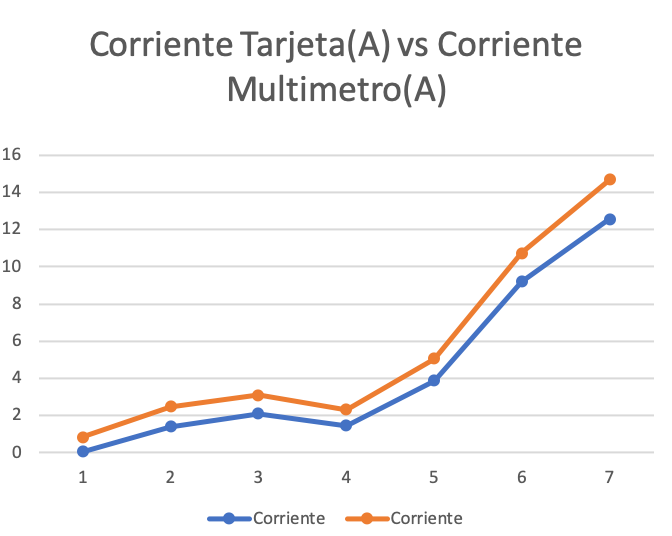
\includegraphics[width = 10cm]{4Resultados/prueba-1.png}
        \caption{ Corriente Tarjeta vs Corriente Multímetro } 
        \label{fig:prueba1}
   \end{center}
\end{figure}

En esta prueba, solo se comparó los registros de corriente rms y voltaje rms que entrega el software con un amperimetro y un osciloscopio midiendo voltaje.
 De igual manera, se calculó un error absoluto y relativo para después ajustar los datos.

 En la figura \ref{fig:prueba1}, la corriente de la tarjeta, tiene presición en su medición más hace falta ajustar su exactitud tomando cómo referencia otro instrumento de medición que se encuentre calibrado.

Según la tabla \ref{tab:resultado1-1}, el promedio de error de voltaje es de un 2\%. El error de corriente es de 177\%, sin embargo ese valor tan alto es debido a que la medicón de una carga que consume baja energía cómo lo es el bombillo, no está dentro de la tolerancia de energía que admite la tarjeta. En la medición del bombillo hay un error relativo del 990\% con respecto a la corriente del amperimetro; por lo tanto, se procede a realizar pruebas con cargas que consuman más energía.
\begin{figure}[H]
  \begin{center}
      \includegraphics[width = 5cm]{4Resultados/prueba1.png}
      \caption{ Cargas utilizadas en la primera prueba } 
      \label{fig:montaje1}
 \end{center}
\end{figure}
\begin{figure}[H]
  \begin{center}
      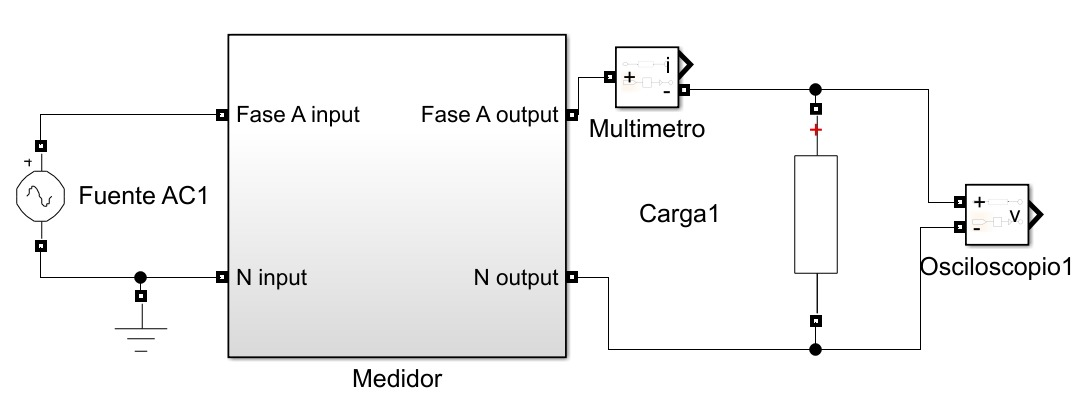
\includegraphics[width = 8cm]{4Resultados/conexion1.jpeg}
      \caption{ Esquema de conexión utilizado en la primera prueba } 
      \label{fig:conexion1}
 \end{center}
\end{figure}
  
\section{Segunda Prueba}
  
En esta prueba se decidió medir todo el ciclo de lavado de una lavadora, con el fin de obtener datos en distintos escenarios los cuales seria llenado, lavado y centrifugado y tener una medición más estable.

Carga:

\begin{itemize}
  \itemsep0em
  \item Lavadora whirlpool de 9.8 A.
\end{itemize}

Ciclos de lavado:

\begin{itemize}
  \itemsep0em
  \item Heavy
  \item Regular
  \item Super wash
  \item Centrifugado
  \item Rinse
  \item Llenado
\end{itemize}
\begin{figure}[H]
  \begin{center}
      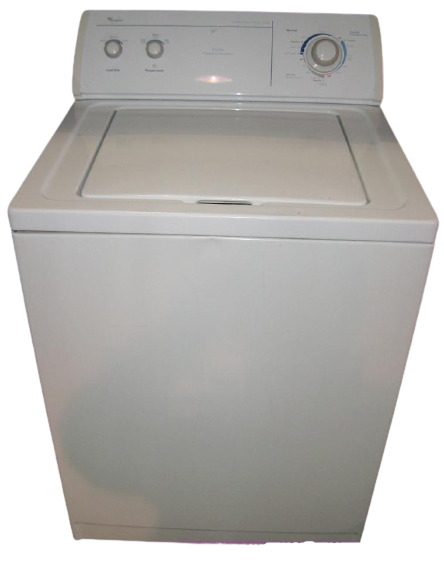
\includegraphics[width = 5cm]{4Resultados/lavadora2.png}
      \caption{ Carga utilizada en la segunda prueba } 
      \label{fig:montaje2}
 \end{center}
\end{figure}
\begin{figure}[H]
  \begin{center}
      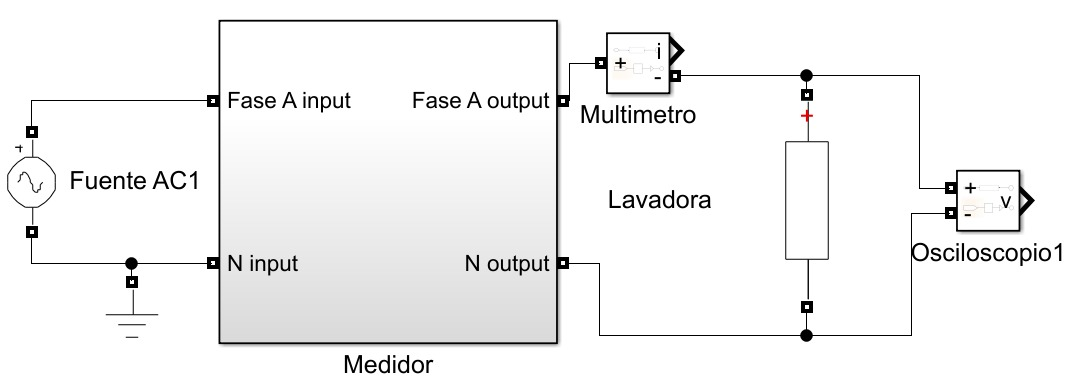
\includegraphics[width = 8cm]{4Resultados/conexion2.jpeg}
      \caption{ Esquema de conexión utilizado en la segunda prueba } 
      \label{fig:conexion2}
 \end{center}
\end{figure}
El análisis se realizó con respecto a los ciclos de lavado y en los todos los ciclos los siguientes datos fueron comunes:

\begin{itemize}
  \itemsep0em
  \item Volatje RMS total con un valor promedio de 121 V en todos los ciclos.
  \item Volatje RMS Fundamental con un valor promedio de 120,97 V en todos los ciclos.
\end{itemize}

\subsection{Análisis en el ciclo heavy}
\begin{figure}[H]
  \hfill
  \subfigure{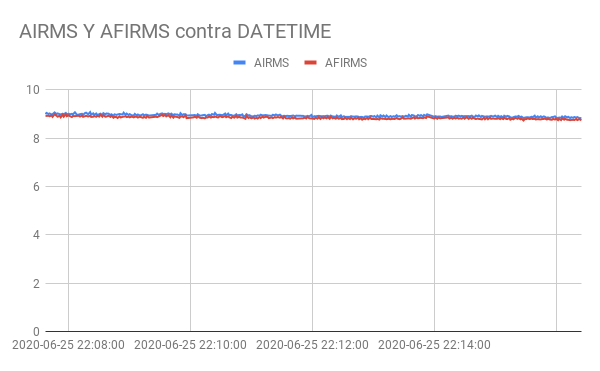
\includegraphics[width=7.5cm]{4Resultados/AIRMS-AFIRMS-Heavy.png}}
  \hfill
  \subfigure{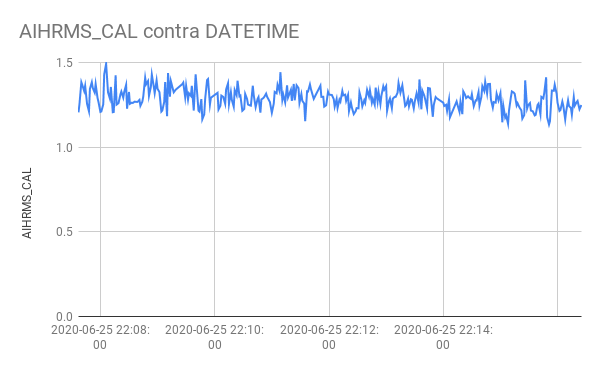
\includegraphics[width=7.5cm]{4Resultados/AIHRMS_CAL-Heavy.png}}
  \hfill
  \caption{AIRMS, AFIRMS Y AIHRMS-CAL VS DATETIME EN EL CICLO HEAVY}
  \end{figure}
\begin{figure}[H]
  \hfill
  \subfigure{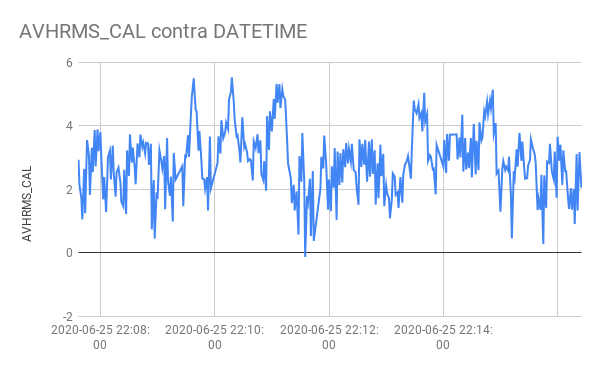
\includegraphics[width=7.5cm]{4Resultados/AVHRMS_CAL-Heavy.png}}
  \hfill
  \subfigure{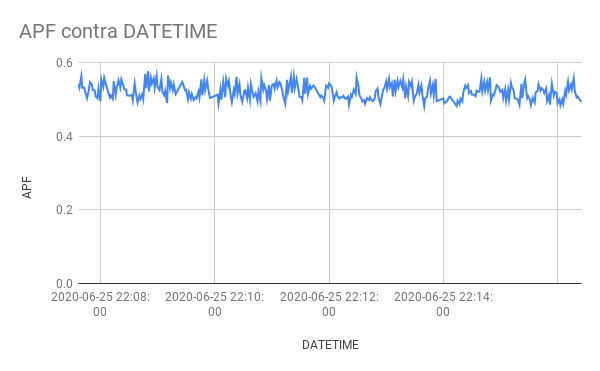
\includegraphics[width=7.5cm]{4Resultados/APF-Heavy.png}}
  \hfill
  \caption{AVHRMS Y APF VS DATETIME EN EL CICLO HEAVY}
  \end{figure}
\begin{figure}[H]
  \hfill
  \subfigure{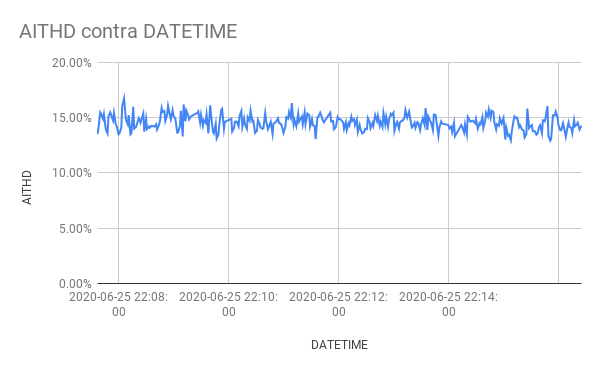
\includegraphics[width=7.5cm]{4Resultados/AITHD-Heavy.png}}
  \hfill
  \subfigure{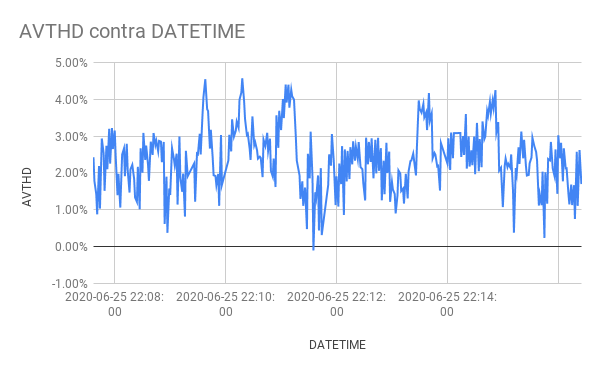
\includegraphics[width=7.5cm]{4Resultados/AVTHD-Heavy.png}}
  \hfill
  \caption{AITHD Y AVTHD VS DATETIME EN EL CICLO HEAVY}
  \end{figure}
\begin{figure}[H]
  \hfill
  \subfigure{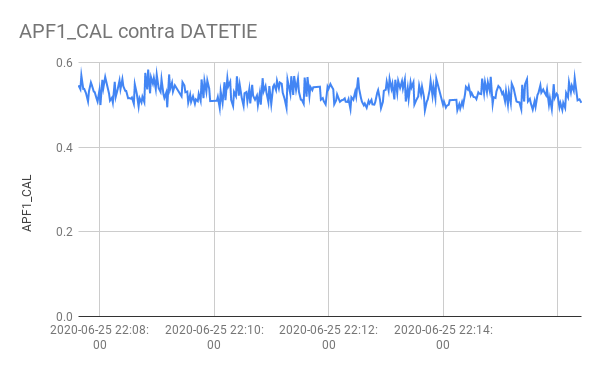
\includegraphics[width=7.5cm]{4Resultados/APF1_CAL-Heavy.png}}
  \hfill
  \subfigure{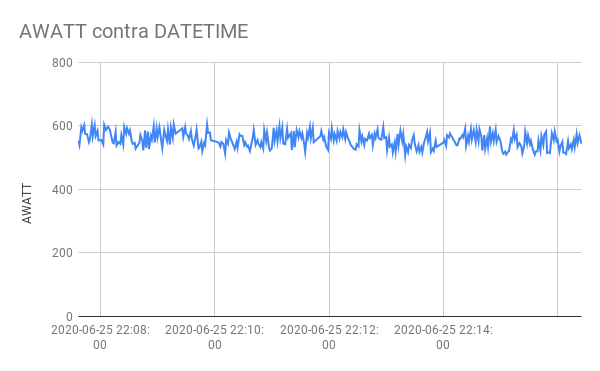
\includegraphics[width=7.5cm]{4Resultados/AWATT-Heavy.png}}
  \hfill
  \caption{APF1-CAL Y AWATT VS DATETIME EN EL CICLO HEAVY}
  \end{figure}
\begin{figure}[H]
  \hfill
  \subfigure{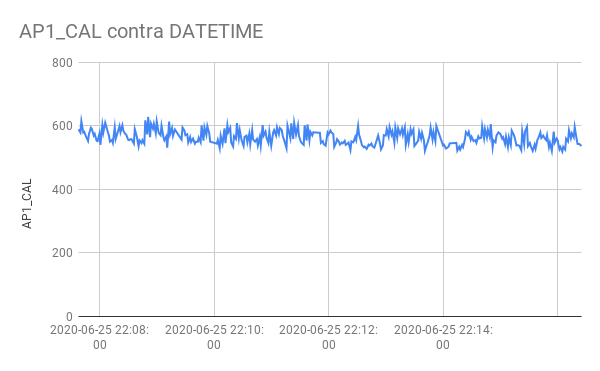
\includegraphics[width=7.5cm]{4Resultados/AP1_CAL-Heavy.png}}
  \hfill
  \subfigure{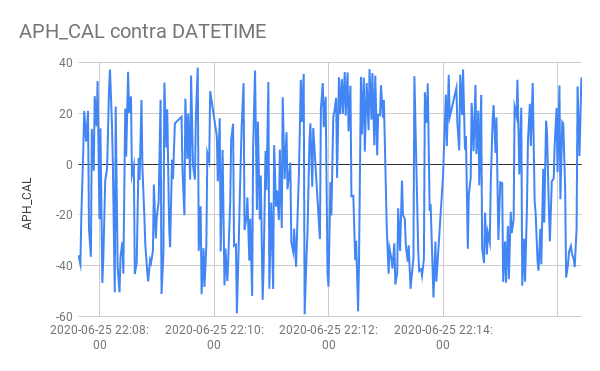
\includegraphics[width=7.5cm]{4Resultados/APH_CAL-Heavy.png}}
  \hfill
  \caption{AP1-CAL Y APH-CAL VS DATETIME EN EL CICLO HEAVY}
  \end{figure}
\begin{figure}[H]
  \hfill
  \subfigure{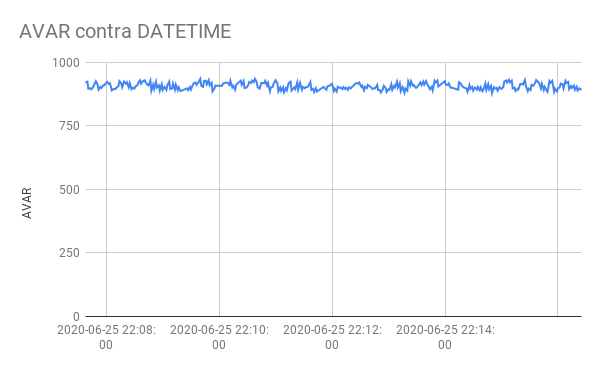
\includegraphics[width=7.5cm]{4Resultados/AVAR-Heavy.png}}
  \hfill
  \subfigure{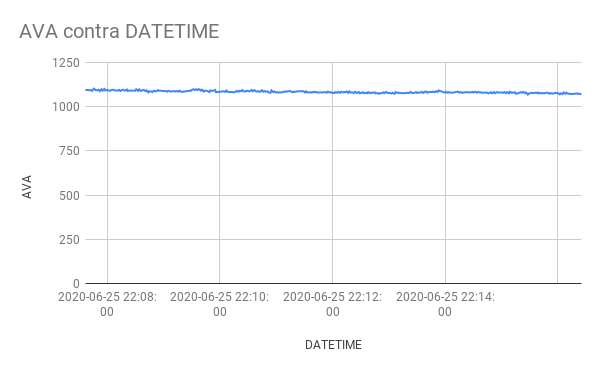
\includegraphics[width=7.5cm]{4Resultados/AVA-Heavy.png}}
  \hfill
  \caption{AVAR Y AVA VS DATETIME EN EL CICLO HEAVY}
  \end{figure}
\begin{figure}[H]
  \hfill
  \subfigure{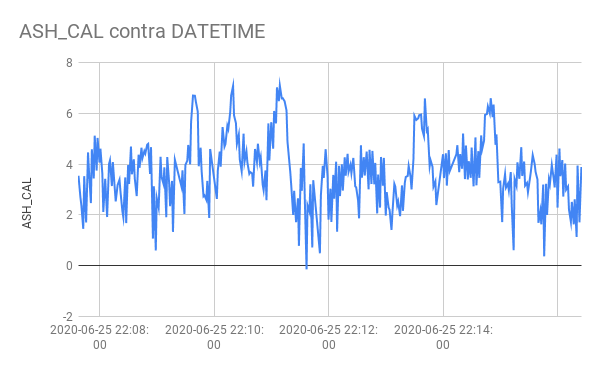
\includegraphics[width=7.5cm]{4Resultados/ASH_CAL-Heavy.png}}
  \hfill
  \subfigure{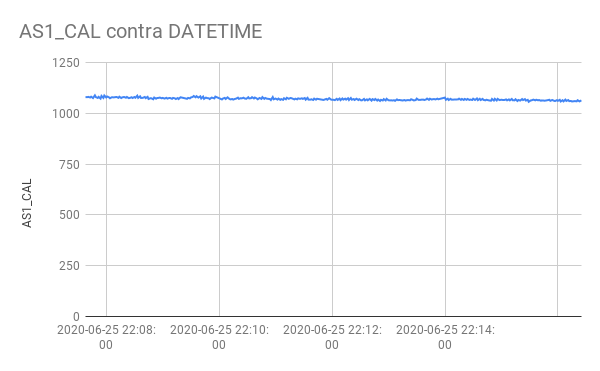
\includegraphics[width=7.5cm]{4Resultados/AS1_CAL-Heavy.png}}
  \hfill
  \caption{ASH-CAL Y AS1-CAL VS DATETIME EN EL CICLO HEAVY}
  \end{figure}
\begin{figure}[H]
  \hfill
  \subfigure{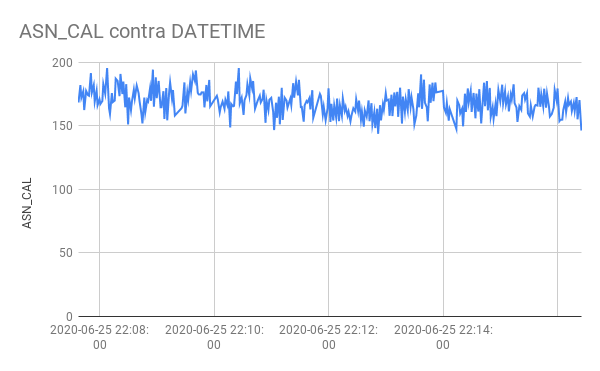
\includegraphics[width=7.5cm]{4Resultados/ASN_CAL-Heavy.png}}
  \hfill
  \subfigure{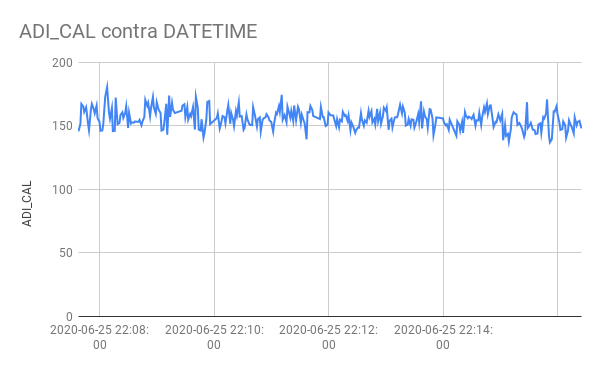
\includegraphics[width=7.5cm]{4Resultados/ADI_CAL-Heavy.png}}
  \hfill
  \caption{ASN-CAL Y ADI-CAL VS DATETIME EN EL CICLO HEAVY}
  \end{figure}
\begin{figure}[H]
  \hfill
  \subfigure{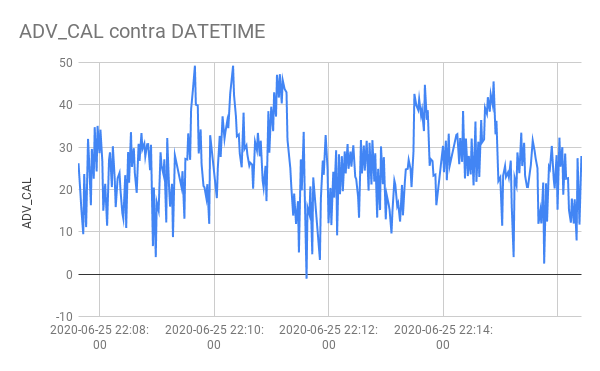
\includegraphics[width=7.5cm]{4Resultados/ADV_CAL-Heavy.png}}
  \hfill
  \subfigure{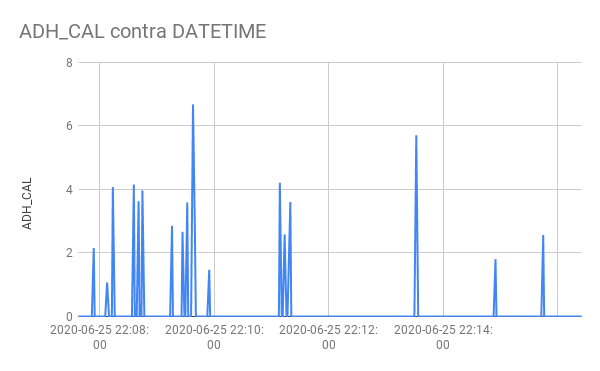
\includegraphics[width=7.5cm]{4Resultados/ADH_CAL-Heavy.png}}
  \hfill
  \caption{ADV-CAL Y ADH-CAL VS DATETIME EN EL CICLO HEAVY}
  \end{figure}
\begin{figure}[H]
  \hfill
  \subfigure{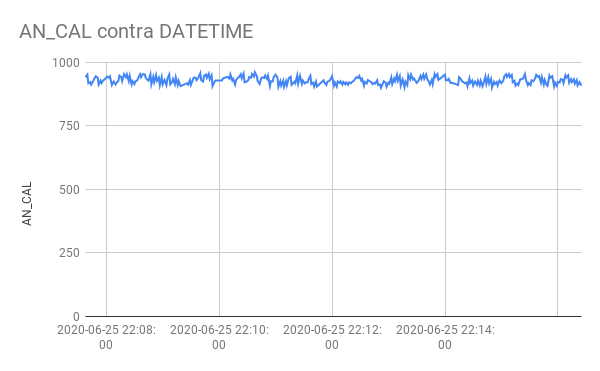
\includegraphics[width=7.5cm]{4Resultados/AN_CAL-Heavy.png}}
  \hfill
  \subfigure{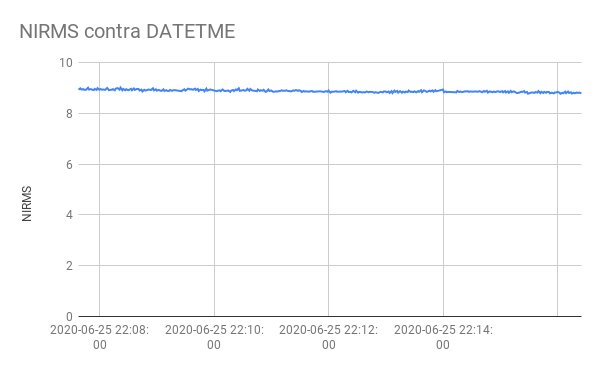
\includegraphics[width=7.5cm]{4Resultados/NIRMS-Heavy.png}}
  \hfill
  \caption{AN-CAL Y NIRMS VS DATETIME EN EL CICLO HEAVY}
  \end{figure}
\begin{figure}[H]
  \hfill
  \subfigure{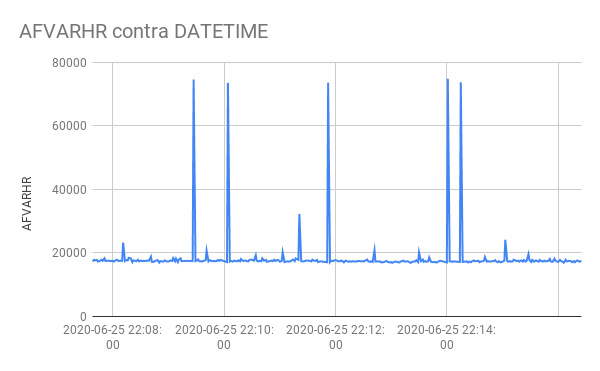
\includegraphics[width=7.5cm]{4Resultados/AFVARHR-Heavy.png}}
  \hfill
  \subfigure{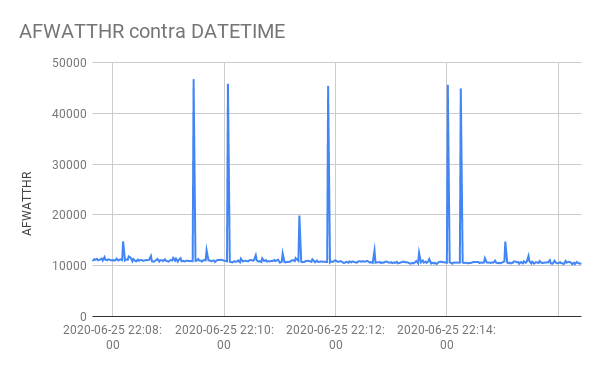
\includegraphics[width=7.5cm]{4Resultados/AFWATTHR-Heavy.png}}
  \hfill
  \caption{AFVARHR Y AFWATTHR VS DATETIME EN EL CICLO HEAVY}
  \end{figure}
\begin{figure}[H]
  \hfill
  \subfigure{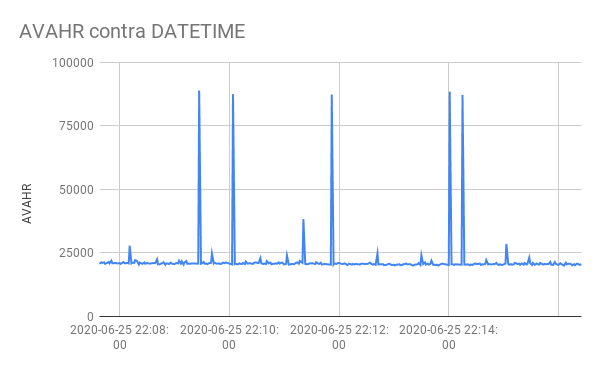
\includegraphics[width=7.5cm]{4Resultados/AVAHR-Heavy.png}}
  \hfill
  \subfigure{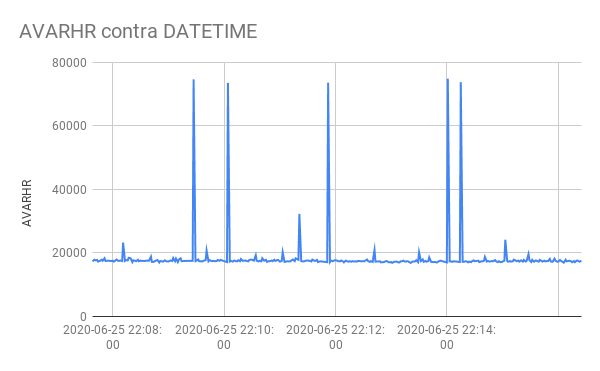
\includegraphics[width=7.5cm]{4Resultados/AVARHR-Heavy.png}}
  \hfill
  \caption{AVAHR Y AVARHR VS DATETIME EN EL CICLO HEAVY}
  \end{figure}
\begin{figure}[H]
  \hfill
  \subfigure{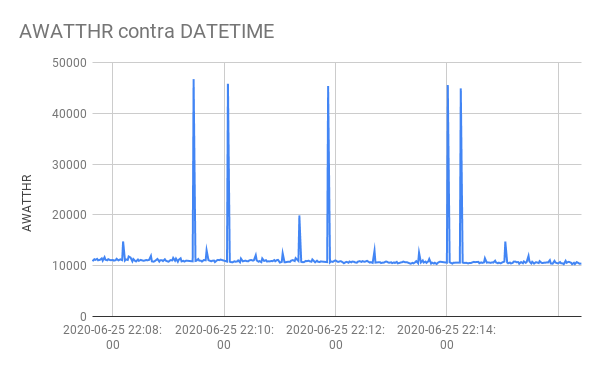
\includegraphics[width=7.5cm]{4Resultados/AWATTHR-Heavy.png}}
  \hfill
  \caption{AWATTHR VS DATETIME EN EL CICLO HEAVY}
  \end{figure}
\subsection{Análisis en el ciclo regular}
\begin{figure}[H]
  \hfill
  \subfigure{\includegraphics[width=7.5cm]{4Resultados/AIRMS-AFIRMS-Regular.png}}
  \hfill
  \subfigure{\includegraphics[width=7.5cm]{4Resultados/AIHRMS_CAL-Regular.png}}
  \hfill
  \caption{AIRMS, AFIRMS Y AIHRMS-CAL VS DATETIME EN EL CICLO REGULAR}
  \end{figure}
\begin{figure}[H]
  \hfill
  \subfigure{\includegraphics[width=7.5cm]{4Resultados/AVHRMS_CAL-Regular.png}}
  \hfill
  \subfigure{\includegraphics[width=7.5cm]{4Resultados/APF-Regular.png}}
  \hfill
  \caption{AVHRMS Y APF VS DATETIME EN EL CICLO REGULAR}
  \end{figure}
\begin{figure}[H]
  \hfill
  \subfigure{\includegraphics[width=7.5cm]{4Resultados/AITHD-Regular.png}}
  \hfill
  \subfigure{\includegraphics[width=7.5cm]{4Resultados/AVTHD-Regular.png}}
  \hfill
  \caption{AITHD Y AVTHD VS DATETIME EN EL CICLO REGULAR}
  \end{figure}
\begin{figure}[H]
  \hfill
  \subfigure{\includegraphics[width=7.5cm]{4Resultados/APF1_CAL-Regular.png}}
  \hfill
  \subfigure{\includegraphics[width=7.5cm]{4Resultados/AWATT-Regular.png}}
  \hfill
  \caption{APF1-CAL Y AWATT VS DATETIME EN EL CICLO REGULAR}
  \end{figure}
\begin{figure}[H]
  \hfill
  \subfigure{\includegraphics[width=7.5cm]{4Resultados/AP1_CAL-Regular.png}}
  \hfill
  \subfigure{\includegraphics[width=7.5cm]{4Resultados/APH_CAL-Regular.png}}
  \hfill
  \caption{AP1-CAL Y APH-CAL VS DATETIME EN EL CICLO REGULAR}
  \end{figure}
\begin{figure}[H]
  \hfill
  \subfigure{\includegraphics[width=7.5cm]{4Resultados/AVAR-Regular.png}}
  \hfill
  \subfigure{\includegraphics[width=7.5cm]{4Resultados/AVA-Regular.png}}
  \hfill
  \caption{AVAR Y AVA VS DATETIME EN EL CICLO REGULAR}
  \end{figure}
\begin{figure}[H]
  \hfill
  \subfigure{\includegraphics[width=7.5cm]{4Resultados/ASH_CAL-Regular.png}}
  \hfill
  \subfigure{\includegraphics[width=7.5cm]{4Resultados/AS1_CAL-Regular.png}}
  \hfill
  \caption{ASH-CAL Y AS1-CAL VS DATETIME EN EL CICLO REGULAR}
  \end{figure}
\begin{figure}[H]
  \hfill
  \subfigure{\includegraphics[width=7.5cm]{4Resultados/ASN_CAL-Regular.png}}
  \hfill
  \subfigure{\includegraphics[width=7.5cm]{4Resultados/ADI_CAL-Regular.png}}
  \hfill
  \caption{ASN-CAL Y ADI-CAL VS DATETIME EN EL CICLO REGULAR}
  \end{figure}
\begin{figure}[H]
  \hfill
  \subfigure{\includegraphics[width=7.5cm]{4Resultados/ADV_CAL-Regular.png}}
  \hfill
  \subfigure{\includegraphics[width=7.5cm]{4Resultados/ADH_CAL-Regular.png}}
  \hfill
  \caption{ADV-CAL Y ADH-CAL VS DATETIME EN EL CICLO REGULAR}
  \end{figure}
\begin{figure}[H]
  \hfill
  \subfigure{\includegraphics[width=7.5cm]{4Resultados/AN_CAL-Regular.png}}
  \hfill
  \subfigure{\includegraphics[width=7.5cm]{4Resultados/NIRMS-Regular.png}}
  \hfill
  \caption{AN-CAL Y NIRMS VS DATETIME EN EL CICLO REGULAR}
  \end{figure}
\begin{figure}[H]
  \hfill
  \subfigure{\includegraphics[width=7.5cm]{4Resultados/AFVARHR-Regular.png}}
  \hfill
  \subfigure{\includegraphics[width=7.5cm]{4Resultados/AFWATTHR-Regular.png}}
  \hfill
  \caption{AFVARHR Y AFWATTHR VS DATETIME EN EL CICLO REGULAR}
  \end{figure}
\begin{figure}[H]
  \hfill
  \subfigure{\includegraphics[width=7.5cm]{4Resultados/AVAHR-Regular.png}}
  \hfill
  \subfigure{\includegraphics[width=7.5cm]{4Resultados/AVARHR-Regular.png}}
  \hfill
  \caption{AVAHR Y AVARHR VS DATETIME EN EL CICLO REGULAR}
  \end{figure}
\begin{figure}[H]
  \hfill
  \subfigure{\includegraphics[width=7.5cm]{4Resultados/AWATTHR-Regular.png}}
  \hfill
  \caption{AWATTHR VS DATETIME EN EL CICLO REGULAR}
  \end{figure}
\subsection{Análisis en el ciclo super wash}
\begin{figure}[H]
  \hfill
  \subfigure{\includegraphics[width=7.5cm]{4Resultados/AIRMS-AFIRMS-SuperWash.png}}
  \hfill
  \subfigure{\includegraphics[width=7.5cm]{4Resultados/AIHRMS_CAL-SuperWash.png}}
  \hfill
  \caption{AIRMS, AFIRMS Y AIHRMS-CAL VS DATETIME EN EL CICLO SUPER WASH}
  \end{figure}
\begin{figure}[H]
  \hfill
  \subfigure{\includegraphics[width=7.5cm]{4Resultados/AVHRMS_CAL-SuperWash.png}}
  \hfill
  \subfigure{\includegraphics[width=7.5cm]{4Resultados/APF-SuperWash.png}}
  \hfill
  \caption{AVHRMS Y APF VS DATETIME EN EL CICLO SUPER WASH}
  \end{figure}
\begin{figure}[H]
  \hfill
  \subfigure{\includegraphics[width=7.5cm]{4Resultados/AITHD-SuperWash.png}}
  \hfill
  \subfigure{\includegraphics[width=7.5cm]{4Resultados/AVTHD-SuperWash.png}}
  \hfill
  \caption{AITHD Y AVTHD VS DATETIME EN EL CICLO SUPER WASH}
  \end{figure}
\begin{figure}[H]
  \hfill
  \subfigure{\includegraphics[width=7.5cm]{4Resultados/APF1_CAL-SuperWash.png}}
  \hfill
  \subfigure{\includegraphics[width=7.5cm]{4Resultados/AWATT-SuperWash.png}}
  \hfill
  \caption{APF1-CAL Y AWATT VS DATETIME EN EL CICLO SUPER WASH}
  \end{figure}
\begin{figure}[H]
  \hfill
  \subfigure{\includegraphics[width=7.5cm]{4Resultados/AP1_CAL-SuperWash.png}}
  \hfill
  \subfigure{\includegraphics[width=7.5cm]{4Resultados/APH_CAL-SuperWash.png}}
  \hfill
  \caption{AP1-CAL Y APH-CAL VS DATETIME EN EL CICLO SUPER WASH}
  \end{figure}
\begin{figure}[H]
  \hfill
  \subfigure{\includegraphics[width=7.5cm]{4Resultados/AVAR-SuperWash.png}}
  \hfill
  \subfigure{\includegraphics[width=7.5cm]{4Resultados/AVA-SuperWash.png}}
  \hfill
  \caption{AVAR Y AVA VS DATETIME EN EL CICLO SUPER WASH}
  \end{figure}
\begin{figure}[H]
  \hfill
  \subfigure{\includegraphics[width=7.5cm]{4Resultados/ASH_CAL-SuperWash.png}}
  \hfill
  \subfigure{\includegraphics[width=7.5cm]{4Resultados/AS1_CAL-SuperWash.png}}
  \hfill
  \caption{ASH-CAL Y AS1-CAL VS DATETIME EN EL CICLO SUPER WASH}
  \end{figure}
\begin{figure}[H]
  \hfill
  \subfigure{\includegraphics[width=7.5cm]{4Resultados/ASN_CAL-SuperWash.png}}
  \hfill
  \subfigure{\includegraphics[width=7.5cm]{4Resultados/ADI_CAL-SuperWash.png}}
  \hfill
  \caption{ASN-CAL Y ADI-CAL VS DATETIME EN EL CICLO SUPER WASH}
  \end{figure}
\begin{figure}[H]
  \hfill
  \subfigure{\includegraphics[width=7.5cm]{4Resultados/ADV_CAL-SuperWash.png}}
  \hfill
  \subfigure{\includegraphics[width=7.5cm]{4Resultados/ADH_CAL-SuperWash.png}}
  \hfill
  \caption{ADV-CAL Y ADH-CAL VS DATETIME EN EL CICLO SUPER WASH}
  \end{figure}
\begin{figure}[H]
  \hfill
  \subfigure{\includegraphics[width=7.5cm]{4Resultados/AN_CAL-SuperWash.png}}
  \hfill
  \subfigure{\includegraphics[width=7.5cm]{4Resultados/NIRMS-SuperWash.png}}
  \hfill
  \caption{AN-CAL Y NIRMS VS DATETIME EN EL CICLO SUPER WASH}
  \end{figure}
\begin{figure}[H]
  \hfill
  \subfigure{\includegraphics[width=7.5cm]{4Resultados/AFVARHR-SuperWash.png}}
  \hfill
  \subfigure{\includegraphics[width=7.5cm]{4Resultados/AFWATTHR-SuperWash.png}}
  \hfill
  \caption{AFVARHR Y AFWATTHR VS DATETIME EN EL CICLO SUPER WASH}
  \end{figure}
\begin{figure}[H]
  \hfill
  \subfigure{\includegraphics[width=7.5cm]{4Resultados/AVAHR-SuperWash.png}}
  \hfill
  \subfigure{\includegraphics[width=7.5cm]{4Resultados/AVARHR-SuperWash.png}}
  \hfill
  \caption{AVAHR Y AVARHR VS DATETIME EN EL CICLO SUPER WASH}
  \end{figure}
\begin{figure}[H]
  \hfill
  \subfigure{\includegraphics[width=7.5cm]{4Resultados/AWATTHR-SuperWash.png}}
  \hfill
  \caption{AWATTHR VS DATETIME EN EL CICLO SUPER WASH}
  \end{figure}
\subsection{Análisis en el ciclo centrifugado}
\begin{figure}[H]
  \hfill
  \subfigure{\includegraphics[width=7.5cm]{4Resultados/AIRMS-AFIRMS-Centrifugado.png}}
  \hfill
  \subfigure{\includegraphics[width=7.5cm]{4Resultados/AIHRMS_CAL-Centrifugado.png}}
  \hfill
  \caption{AIRMS, AFIRMS Y AIHRMS-CAL VS DATETIME EN EL CICLO CENTRIFUGADO}
  \end{figure}
\begin{figure}[H]
  \hfill
  \subfigure{\includegraphics[width=7.5cm]{4Resultados/AVHRMS_CAL-Centrifugado.png}}
  \hfill
  \subfigure{\includegraphics[width=7.5cm]{4Resultados/APF-Centrifugado.png}}
  \hfill
  \caption{AVHRMS Y APF VS DATETIME EN EL CICLO CENTRIFUGADO}
  \end{figure}
\begin{figure}[H]
  \hfill
  \subfigure{\includegraphics[width=7.5cm]{4Resultados/AITHD-Centrifugado.png}}
  \hfill
  \subfigure{\includegraphics[width=7.5cm]{4Resultados/AVTHD-Centrifugado.png}}
  \hfill
  \caption{AITHD Y AVTHD VS DATETIME EN EL CICLO CENTRIFUGADO}
  \end{figure}
\begin{figure}[H]
  \hfill
  \subfigure{\includegraphics[width=7.5cm]{4Resultados/APF1_CAL-Centrifugado.png}}
  \hfill
  \subfigure{\includegraphics[width=7.5cm]{4Resultados/AWATT-Centrifugado.png}}
  \hfill
  \caption{APF1-CAL Y AWATT VS DATETIME EN EL CICLO CENTRIFUGADO}
  \end{figure}
\begin{figure}[H]
  \hfill
  \subfigure{\includegraphics[width=7.5cm]{4Resultados/AP1_CAL-Centrifugado.png}}
  \hfill
  \subfigure{\includegraphics[width=7.5cm]{4Resultados/APH_CAL-Centrifugado.png}}
  \hfill
  \caption{AP1-CAL Y APH-CAL VS DATETIME EN EL CICLO CENTRIFUGADO}
  \end{figure}
\begin{figure}[H]
  \hfill
  \subfigure{\includegraphics[width=7.5cm]{4Resultados/AVAR-Centrifugado.png}}
  \hfill
  \subfigure{\includegraphics[width=7.5cm]{4Resultados/AVA-Centrifugado.png}}
  \hfill
  \caption{AVAR Y AVA VS DATETIME EN EL CICLO CENTRIFUGADO}
  \end{figure}
\begin{figure}[H]
  \hfill
  \subfigure{\includegraphics[width=7.5cm]{4Resultados/ASH_CAL-Centrifugado.png}}
  \hfill
  \subfigure{\includegraphics[width=7.5cm]{4Resultados/AS1_CAL-Centrifugado.png}}
  \hfill
  \caption{ASH-CAL Y AS1-CAL VS DATETIME EN EL CICLO CENTRIFUGADO}
  \end{figure}
\begin{figure}[H]
  \hfill
  \subfigure{\includegraphics[width=7.5cm]{4Resultados/ASN_CAL-Centrifugado.png}}
  \hfill
  \subfigure{\includegraphics[width=7.5cm]{4Resultados/ADI_CAL-Centrifugado.png}}
  \hfill
  \caption{ASN-CAL Y ADI-CAL VS DATETIME EN EL CICLO CENTRIFUGADO}
  \end{figure}
\begin{figure}[H]
  \hfill
  \subfigure{\includegraphics[width=7.5cm]{4Resultados/ADV_CAL-Centrifugado.png}}
  \hfill
  \subfigure{\includegraphics[width=7.5cm]{4Resultados/ADH_CAL-Centrifugado.png}}
  \hfill
  \caption{ADV-CAL Y ADH-CAL VS DATETIME EN EL CICLO CENTRIFUGADO}
  \end{figure}
\begin{figure}[H]
  \hfill
  \subfigure{\includegraphics[width=7.5cm]{4Resultados/AN_CAL-Centrifugado.png}}
  \hfill
  \subfigure{\includegraphics[width=7.5cm]{4Resultados/NIRMS-Centrifugado.png}}
  \hfill
  \caption{AN-CAL Y NIRMS VS DATETIME EN EL CICLO CENTRIFUGADO}
  \end{figure}
\begin{figure}[H]
  \hfill
  \subfigure{\includegraphics[width=7.5cm]{4Resultados/AFVARHR-Centrifugado.png}}
  \hfill
  \subfigure{\includegraphics[width=7.5cm]{4Resultados/AFWATTHR-Centrifugado.png}}
  \hfill
  \caption{AFVARHR Y AFWATTHR VS DATETIME EN EL CICLO CENTRIFUGADO}
  \end{figure}
\begin{figure}[H]
  \hfill
  \subfigure{\includegraphics[width=7.5cm]{4Resultados/AVAHR-Centrifugado.png}}
  \hfill
  \subfigure{\includegraphics[width=7.5cm]{4Resultados/AVARHR-Centrifugado.png}}
  \hfill
  \caption{AVAHR Y AVARHR VS DATETIME EN EL CICLO CENTRIFUGADO}
  \end{figure}
\begin{figure}[H]
  \hfill
  \subfigure{\includegraphics[width=7.5cm]{4Resultados/AWATTHR-Centrifugado.png}}
  \hfill
  \caption{AWATTHR VS DATETIME EN EL CICLO CENTRIFUGADO}
  \end{figure}
\subsection{Análisis en el ciclo rinse}
\begin{figure}[H]
  \hfill
  \subfigure{\includegraphics[width=7.5cm]{4Resultados/AIRMS-AFIRMS-Rinse.png}}
  \hfill
  \subfigure{\includegraphics[width=7.5cm]{4Resultados/AIHRMS_CAL-Rinse.png}}
  \hfill
  \caption{AIRMS, AFIRMS Y AIHRMS-CAL VS DATETIME EN EL CICLO RINSE}
  \end{figure}
\begin{figure}[H]
  \hfill
  \subfigure{\includegraphics[width=7.5cm]{4Resultados/AVHRMS_CAL-Rinse.png}}
  \hfill
  \subfigure{\includegraphics[width=7.5cm]{4Resultados/APF-Rinse.png}}
  \hfill
  \caption{AVHRMS Y APF VS DATETIME EN EL CICLO RINSE}
  \end{figure}
\begin{figure}[H]
  \hfill
  \subfigure{\includegraphics[width=7.5cm]{4Resultados/AITHD-Rinse.png}}
  \hfill
  \subfigure{\includegraphics[width=7.5cm]{4Resultados/AVTHD-Rinse.png}}
  \hfill
  \caption{AITHD Y AVTHD VS DATETIME EN EL CICLO RINSE}
  \end{figure}
\begin{figure}[H]
  \hfill
  \subfigure{\includegraphics[width=7.5cm]{4Resultados/APF1_CAL-Rinse.png}}
  \hfill
  \subfigure{\includegraphics[width=7.5cm]{4Resultados/AWATT-Rinse.png}}
  \hfill
  \caption{APF1-CAL Y AWATT VS DATETIME EN EL CICLO RINSE}
  \end{figure}
\begin{figure}[H]
  \hfill
  \subfigure{\includegraphics[width=7.5cm]{4Resultados/AP1_CAL-Rinse.png}}
  \hfill
  \subfigure{\includegraphics[width=7.5cm]{4Resultados/APH_CAL-Rinse.png}}
  \hfill
  \caption{AP1-CAL Y APH-CAL VS DATETIME EN EL CICLO RINSE}
  \end{figure}
\begin{figure}[H]
  \hfill
  \subfigure{\includegraphics[width=7.5cm]{4Resultados/AVAR-Rinse.png}}
  \hfill
  \subfigure{\includegraphics[width=7.5cm]{4Resultados/AVA-Rinse.png}}
  \hfill
  \caption{AVAR Y AVA VS DATETIME EN EL CICLO RINSE}
  \end{figure}
\begin{figure}[H]
  \hfill
  \subfigure{\includegraphics[width=7.5cm]{4Resultados/ASH_CAL-Rinse.png}}
  \hfill
  \subfigure{\includegraphics[width=7.5cm]{4Resultados/AS1_CAL-Rinse.png}}
  \hfill
  \caption{ASH-CAL Y AS1-CAL VS DATETIME EN EL CICLO RINSE}
  \end{figure}
\begin{figure}[H]
  \hfill
  \subfigure{\includegraphics[width=7.5cm]{4Resultados/ASN_CAL-Rinse.png}}
  \hfill
  \subfigure{\includegraphics[width=7.5cm]{4Resultados/ADI_CAL-Rinse.png}}
  \hfill
  \caption{ASN-CAL Y ADI-CAL VS DATETIME EN EL CICLO RINSE}
  \end{figure}
\begin{figure}[H]
  \hfill
  \subfigure{\includegraphics[width=7.5cm]{4Resultados/ADV_CAL-Rinse.png}}
  \hfill
  \subfigure{\includegraphics[width=7.5cm]{4Resultados/ADH_CAL-Rinse.png}}
  \hfill
  \caption{ADV-CAL Y ADH-CAL VS DATETIME EN EL CICLO RINSE}
  \end{figure}
\begin{figure}[H]
  \hfill
  \subfigure{\includegraphics[width=7.5cm]{4Resultados/AN_CAL-Rinse.png}}
  \hfill
  \subfigure{\includegraphics[width=7.5cm]{4Resultados/NIRMS-Rinse.png}}
  \hfill
  \caption{AN-CAL Y NIRMS VS DATETIME EN EL CICLO RINSE}
  \end{figure}
\begin{figure}[H]
  \hfill
  \subfigure{\includegraphics[width=7.5cm]{4Resultados/AFVARHR-Rinse.png}}
  \hfill
  \subfigure{\includegraphics[width=7.5cm]{4Resultados/AFWATTHR-Rinse.png}}
  \hfill
  \caption{AFVARHR Y AFWATTHR VS DATETIME EN EL CICLO RINSE}
  \end{figure}
\begin{figure}[H]
  \hfill
  \subfigure{\includegraphics[width=7.5cm]{4Resultados/AVAHR-Rinse.png}}
  \hfill
  \subfigure{\includegraphics[width=7.5cm]{4Resultados/AVARHR-Rinse.png}}
  \hfill
  \caption{AVAHR Y AVARHR VS DATETIME EN EL CICLO RINSE}
  \end{figure}
\begin{figure}[H]
  \hfill
  \subfigure{\includegraphics[width=7.5cm]{4Resultados/AWATTHR-Rinse.png}}
  \hfill
  \caption{AWATTHR VS DATETIME EN EL CICLO RINSE}
  \end{figure}
\subsection{Análisis en el ciclo llenado}
\begin{figure}[H]
  \hfill
  \subfigure{\includegraphics[width=7.5cm]{4Resultados/AIRMS-AFIRMS-Llenado.png}}
  \hfill
  \subfigure{\includegraphics[width=7.5cm]{4Resultados/AIHRMS_CAL-Llenado.png}}
  \hfill
  \caption{AIRMS, AFIRMS Y AIHRMS-CAL VS DATETIME EN EL CICLO LLENADO}
  \end{figure}
\begin{figure}[H]
  \hfill
  \subfigure{\includegraphics[width=7.5cm]{4Resultados/AVHRMS_CAL-Llenado.png}}
  \hfill
  \subfigure{\includegraphics[width=7.5cm]{4Resultados/APF-Llenado.png}}
  \hfill
  \caption{AVHRMS Y APF VS DATETIME EN EL CICLO LLENADO}
  \end{figure}
\begin{figure}[H]
  \hfill
  \subfigure{\includegraphics[width=7.5cm]{4Resultados/AITHD-Llenado.png}}
  \hfill
  \subfigure{\includegraphics[width=7.5cm]{4Resultados/AVTHD-Llenado.png}}
  \hfill
  \caption{AITHD Y AVTHD VS DATETIME EN EL CICLO LLENADO}
  \end{figure}
\begin{figure}[H]
  \hfill
  \subfigure{\includegraphics[width=7.5cm]{4Resultados/APF1_CAL-Llenado.png}}
  \hfill
  \subfigure{\includegraphics[width=7.5cm]{4Resultados/AWATT-Llenado.png}}
  \hfill
  \caption{APF1-CAL Y AWATT VS DATETIME EN EL CICLO LLENADO}
  \end{figure}
\begin{figure}[H]
  \hfill
  \subfigure{\includegraphics[width=7.5cm]{4Resultados/AP1_CAL-Llenado.png}}
  \hfill
  \subfigure{\includegraphics[width=7.5cm]{4Resultados/APH_CAL-Llenado.png}}
  \hfill
  \caption{AP1-CAL Y APH-CAL VS DATETIME EN EL CICLO LLENADO}
  \end{figure}
\begin{figure}[H]
  \hfill
  \subfigure{\includegraphics[width=7.5cm]{4Resultados/AVAR-Llenado.png}}
  \hfill
  \subfigure{\includegraphics[width=7.5cm]{4Resultados/AVA-Llenado.png}}
  \hfill
  \caption{AVAR Y AVA VS DATETIME EN EL CICLO LLENADO}
  \end{figure}
\begin{figure}[H]
  \hfill
  \subfigure{\includegraphics[width=7.5cm]{4Resultados/ASH_CAL-Llenado.png}}
  \hfill
  \subfigure{\includegraphics[width=7.5cm]{4Resultados/AS1_CAL-Llenado.png}}
  \hfill
  \caption{ASH-CAL Y AS1-CAL VS DATETIME EN EL CICLO LLENADO}
  \end{figure}
\begin{figure}[H]
  \hfill
  \subfigure{\includegraphics[width=7.5cm]{4Resultados/ASN_CAL-Llenado.png}}
  \hfill
  \subfigure{\includegraphics[width=7.5cm]{4Resultados/ADI_CAL-Llenado.png}}
  \hfill
  \caption{ASN-CAL Y ADI-CAL VS DATETIME EN EL CICLO LLENADO}
  \end{figure}
\begin{figure}[H]
  \hfill
  \subfigure{\includegraphics[width=7.5cm]{4Resultados/ADV_CAL-Llenado.png}}
  \hfill
  \subfigure{\includegraphics[width=7.5cm]{4Resultados/ADH_CAL-Llenado.png}}
  \hfill
  \caption{ADV-CAL Y ADH-CAL VS DATETIME EN EL CICLO LLENADO}
  \end{figure}
\begin{figure}[H]
  \hfill
  \subfigure{\includegraphics[width=7.5cm]{4Resultados/AN_CAL-Llenado.png}}
  \hfill
  \subfigure{\includegraphics[width=7.5cm]{4Resultados/NIRMS-Llenado.png}}
  \hfill
  \caption{AN-CAL Y NIRMS VS DATETIME EN EL CICLO LLENADO}
  \end{figure}
\begin{figure}[H]
  \hfill
  \subfigure{\includegraphics[width=7.5cm]{4Resultados/AFVARHR-Llenado.png}}
  \hfill
  \subfigure{\includegraphics[width=7.5cm]{4Resultados/AFWATTHR-Llenado.png}}
  \hfill
  \caption{AFVARHR Y AFWATTHR VS DATETIME EN EL CICLO LLENADO}
  \end{figure}
\begin{figure}[H]
  \hfill
  \subfigure{\includegraphics[width=7.5cm]{4Resultados/AVAHR-Llenado.png}}
  \hfill
  \subfigure{\includegraphics[width=7.5cm]{4Resultados/AVARHR-Llenado.png}}
  \hfill
  \caption{AVAHR Y AVARHR VS DATETIME EN EL CICLO LLENADO}
  \end{figure}
\begin{figure}[H]
  \hfill
  \subfigure{\includegraphics[width=7.5cm]{4Resultados/AWATTHR-Llenado.png}}
  \hfill
  \caption{AWATTHR VS DATETIME EN EL CICLO LLENADO}
  \end{figure}

  Con esta prueba, se obtuvo una caracterización más del medidor, la cuál para un funcionamiento estable y preciso de la tarjeta, es necesario que las cargas consuman como mínimo 1 Amperio, sin embargo, debido a la alta frecuencia con la que el ADE7978 hace la medición, hay ocasiones en que los datos presentan un valor fuera del rango. \\\\
  Completada la prueba monofásica, se procedió a realizar la prueba trifásica desbalanceada con el fin de tener cubierto todos los casos de medición que se planteó en este proyecto.
  \section{Tercer Prueba}

  Para esta prueba se utilizó una red trifásica doméstica y a cada fase se conectó a una carga. las tres cargas son tienen un consumo distinto para así probar y medir el caso trifásico desbalanceado.\\\\
  A continuación se describe las cargas que se usaron:\\
  \begin{itemize}
    \itemsep0em
    \item FASE A - 2 pantallas, 1 cpu, 2 portatiles y una Raspberry.
    \item FASE B - Caminadora eléctrica.
    \item FASE C - Lavadora samsung.
  \end{itemize}
    \begin{figure}[H]
      \begin{center}
          \includegraphics[width = 7.5cm]{4Resultados/prueba2.png}
          \caption{ Cagas utilizadas en la tercera prueba} 
          \label{fig:cargas-3}
     \end{center}
    \end{figure}
    \begin{figure}[H]
      \begin{center}
          \includegraphics[width = 8cm]{4Resultados/conexion3.jpeg}
          \caption{ Esquema de conexión utilizado en la tercera prueba } 
          \label{fig:conexion3}
     \end{center}
    \end{figure}
    \subsection{Resultados de la prueba}
    \begin{figure}[H]
      \hfill
      \subfigure{\includegraphics[width=7.5cm]{4Resultados/corriente-rms.png}}
      \hfill
      \subfigure{\includegraphics[width=7.5cm]{4Resultados/corriente-fundamental.png}}
      \hfill
      \caption{CORRIENTE RMS Y CORRIENTE FUNDAMENTAL}
      \end{figure}

      Las variaciones que se ven en la señal CIRMS es debido a los distintos ciclos que tiene la lavadora mientras realizaba su ciclo de lavado. \\
      La caminadora se le hizo una variación en la velocidad por lo cual se ve una subida en la gráfica de corriente BIRMS.\\
      La carga en la fase A no tuvo ninguna variación durante la medición por lo cual la señal AIRMS es estable.\\
    \begin{figure}[H]
      \hfill
      \subfigure{\includegraphics[width=7.5cm]{4Resultados/corriente-armonica.png}}
      \hfill
      \subfigure{\includegraphics[width=7.5cm]{4Resultados/THDI.png}}
      \hfill
      \caption{CORRIENTE ARMÓNICA Y DISTORSIÓN ARMÓNICA DE CORRIENTE}
      \label{fig:corriente-armonica}
      \end{figure}
      En la gráfica \ref{fig:Voltaje-armonico}, se ve las distorsiones en corriente que presentan las cargas que en los medidores actuales no tienen en cuenta, sin embargo este medidor lo analiza al momento de medir.
    \begin{figure}[H]
      \hfill
      \subfigure{\includegraphics[width=7.5cm]{4Resultados/voltaje-rms.png}}
      \hfill
      \subfigure{\includegraphics[width=7.5cm]{4Resultados/voltaje-fundamental.png}}
      \hfill
      \caption{VOLTAJE RMS Y VOLTAJE FUNDAMENTAL}
      \end{figure}
    \begin{figure}[H]
      \hfill
      \subfigure{\includegraphics[width=7.5cm]{4Resultados/voltaje-armonico.png}}
      \hfill
      \subfigure{\includegraphics[width=7.5cm]{4Resultados/THDV.png}}
      \hfill
      \caption{VOLTAJE ARMÓNICA Y DISTORSIÓN ARMÓNICA DE VOLTAJE}
      \label{fig:Voltaje-armonico}
      \end{figure}

      En la gráfica \ref{fig:Voltaje-armonico}, se ve las distorsiones en voltaje que presentan las cargas que en los medidores actuales no tienen en cuenta, sin embargo este medidor lo analiza al momento de medir.
    \begin{figure}[H]
      \hfill
      \subfigure{\includegraphics[width=7.5cm]{4Resultados/factor-potencia-total.png}}
      \hfill
      \subfigure{\includegraphics[width=7.5cm]{4Resultados/factor-potencia-fundamental.png}}
      \hfill
      \caption{FACTOR DE POTENCIA TOTAL Y FACTOR DE POTENCIA FUNDAMENTAL}
      \label{fig:factor-potencia}
      \end{figure}
      En la gráfica \ref{fig:factor-potencia}, se evidencia un error en la medición del factor de potencia ya que hay valores superiores a 1.
    
    \begin{figure}[H]
      \hfill
      \subfigure{\includegraphics[width=7.5cm]{4Resultados/potencia-aparente-total.png}}
      \hfill
      \subfigure{\includegraphics[width=7.5cm]{4Resultados/potencia-aparente-fundamental.png}}
      \hfill
      \caption{POTENCIA APARENTE TOTAL Y POTENCIA APARENTE FUNDAMENTAL}
      \end{figure}
    \begin{figure}[H]
      \hfill
      \subfigure{\includegraphics[width=7.5cm]{4Resultados/potencia-aparente-armonica.png}}
      \hfill
      \subfigure{\includegraphics[width=7.5cm]{4Resultados/angulo-desfase.png}}
      \hfill
      \caption{POTENCIA APARENTE ARMÓNICA Y ÁNGULO DE DESFASE ENTRE FASES}
      \end{figure}

    En la gráfica de los ángulos de desfase, las etiquetas se interpretan de la siguiente manera:
    \begin{itemize}
      \itemsep0em
      \item ANGLE 0 - ángulo de desfase entre la fase A y B.
      \item ANGLE 1 - ángulo de desfase entre la fase B y C.
      \item ANGLE 2 - ángulo de desfase entre la fase C y A.
    \end{itemize}
    \begin{figure}[H]
      \hfill
      \subfigure{\includegraphics[width=7.5cm]{4Resultados/potencia-activa-total.png}}
      \hfill
      \subfigure{\includegraphics[width=7.5cm]{4Resultados/potencia-activa-armonica.png}}
      \hfill
      \caption{POTENCIA ACTIVA TOTAL Y POTENCIA ACTIVA ARMÓNICA}
      \end{figure}
    \begin{figure}[H]
      \hfill
      \subfigure{\includegraphics[width=7.5cm]{4Resultados/current-distortion-var.png}}
      \hfill
      \subfigure{\includegraphics[width=7.5cm]{4Resultados/voltage-distortion-var.png}}
      \hfill
      \caption{DISTORSIÓN DE POTENCIA (VAR) EN CORRIENTE Y VOLTAJE}
      \end{figure}
    \begin{figure}[H]
      \hfill
      \subfigure{\includegraphics[width=7.5cm]{4Resultados/NIRMS.png}}
      \hfill
      \subfigure{\includegraphics[width=7.5cm]{4Resultados/potencia-noactiva-var.png}}
      \hfill
      \caption{CORRIENTE RMS EN NEUTRO Y POTENCIA (VAR) NO ACTIVA}
      \end{figure}

      En las gráficas de potencia, se analiza que el consumo de energía es acorde a la corriente que consume la carga.

  
%{\clearpage}
\chapter{Impacto social}
Se deben incluir tantos cap\'{\i}tulos como se requieran; sin embargo, se recomienda que la tesis  o trabajo de investigaci\'{o}n tenga un m\'{\i}nimo 3 cap\'{\i}tulos y m\'{a}ximo de 6 cap\'{\i}tulos (incluyendo las conclusiones).\\
%{\clearpage}
\chapter{ Conclusiones}

\begin{itemize}
    \itemsep0em
    % \item El proyecto propuesto, como ya se explicó, consiste en cuatro fases, mediante cada una de ellas se obtiene información de mucha utilidad para cumplir los objetivos de este trabajo. Como primera fase, se explican los parámetros, variables y formulas necesarias para emplear la norma IEEE14-59-2010 (1459-2010 IEEE Standard Definitions for the Measurement of Electric Power Quantities Under Sinusoidal, Nonsinusoidal, Balanced, or Unbalanced Conditions., n.d.), la cuál es la base para lograr el objetivo principal del proyecto. Define la forma en la que se debe medir cualquier tipo de carga monfásica y trifásica; la siguiente etapa trata de la identifiación de un procesador que lea y descomponga la señal de voltaje y corriente de cada fase y así poder hacer el tratamiento de datos con el estandar IEEE 1459; luego continúa la implementación del hardware garantizando una conexión segura y optima; posteriormente se desarrolla un software acorde al proyecto que permita tomar las mediciones, realizar el tratamiento de datos y enviarlos al servidor para al final ser visualizados por medio de una página web; con esta información, se crea un analísis de datos que resume toda la información obtenida y procesada donde se muestra un escenario de la vida cotidiana y finalmente permite ver las distorsiones que la carga presenta y así obtener una medición más precisa que es lo que se busca en este proyecto.
    % \item Por otro lado, se planteo una métodología que describe el paso a paso de las actividades a desarrollar y llevar a cabo la implementación de un medidor de energía trifásica para sistemas eléctricos no lineales basado en la norma IEEE14-59-2010 (1459-2010 IEEE Standard Definitions for the Measurement of Electric Power Quantities Under Sinusoidal, Nonsinusoidal, Balanced, or Unbalanced Conditions., n.d.). Asimismo, se define y se suministra las herramientas necesarias para la recopilación y estructuración del medidor, se precisan los objetivos y los resultados que se conseguirán al final de cada fase.
    % \item Tanto el proyecto como la métodología se implementaron con un foco orientado a la optimización y mejoramiento de la medición energética y debido a su conectividad con internet, abre una gran oportunidad para que sistemas de redes eléctricas inteligentes o fuentes de energía renovable puedan utilizar este sistema de medición.
    % \item Cómo se evidenció en la primera prueba del medidor, al momento de medir el bombillo con un consumo de 9 vatios, el medidor presentó un alto porcentaje de error en su medición, por lo tanto se optó por realizar pruebas con cargas que tuvieran un mayor consumo y con cargas de 1 A, el medidor empieza a funcionar de manera optima, por lo tanto el rango de medición del medidor es de 1 A a 15 A.
    % \item El medidor se diseñó con la shunt propuesta debido a que fue la mas adsequible en el momento, sin embargo, la ventaja de este medidor es que se puede adaptar a cualquier tamaño de medicion tan solo cambiando la resistencia shunt y asegurando un voltaje de entrada en la dsp de +- 31.25mV haciendo el dispositivo muy versatil para implementar en cualquier sector.
    % \item El ade-7978 no realiza el análisis de estandar IEEE14-59-2010 (1459-2010 IEEE Standard Definitions for the Measurement of Electric Power Quantities Under Sinusoidal, Nonsinusoidal, Balanced, or Unbalanced Conditions., n.d.), sin embargo, entrega los datos necesarios para realizar el tratamiento de datos a travez de un procesador de datos y así cumplir con el estandar.
    % \item Se optó por usar el lenguaje de progrmación c++ ya que es un lenguaje de programación de bajo nivel, permite acceder mejor a los registros y hacer un mejor uso de la memoria en el procesador. En el desarrollo de la página web, se usó angular ya que este cuenta con el lenguaje Typescript y nos permite tipar los datos con el fin de tener un sistema robusto.
    % \item El medidor tiene conectvidad a internet, por lo tanto el proyecto cuenta con IoT (internet de las cosas) y esto implica que el análisis que tuvo en su arquitectura de software fuera complejo. Para un mejor desempeño es necesario contar con  altos conocimientos en arquitectura de software para garantizar que no haya perdida de datos, sin embargo no se posee dicho conocimiento por lo que queda cómo mejora del proyecto ya que este presenta pequeñas fallas en su medición y es debido a que la frecuencia con la que el ADE 7978 adquiere los datos es muy alta y no contamos con un procesador que vaya a la misma velocidad y a la vez cuente con tarjeta wifi para enviar los datos al servidor.
    % \item Debido a que se terminó el desarrollo del medidor en una epoca de pandemia mundial por el covid-19, no fue posible realizar una comparación de mediciones con el AEMC 45b y el circutor, sin embargo se creó un banco de datos y pruebas, el cuál tiene todas las mediciones que se tomaron; posteriormente este banco permite a futuro realizar una comparación con los medidores de referencia propuestos.
    % \item Durante el desarrollo del proyecto, se evidenció que la planeación que se hizo en el anteproyecto estuvo mal diseñada ya que se tuvieron inconvenientes como el de escoger el dispositivo correcto que cumpliera con la norma IEEE 1459, tiempo de compra y respuesta por parte del FODEIN para la financiación del proyecto, el lenguaje de programación, protocolo de comunicación y representación de los datos del dispositivo. Por lo tanto, los inconvenientes ya mencionados impactaron en el tiempo de entrega del proyecto y en su complejidad. El objetivo principal es emplear la norma IEEE 1459 en un medidor de energía, sin embargo, la arquitectura de hardware y software paso a ser más compleja debido a que los datos se mostraron por medio de una página web en donde se tuvieron que analizar factores como, velocidad de ejecución, tiempo de respuesta en envío y lectura de datos y comunicación de dispositivos entre otros. Acorde a todo lo que no se tuvo en cuenta en la planeación, se llegó a la conclusión que este proyecto de grado cumple con todos los requerimientos que una tesis de pregrado y postgrado a su vez requieren.
    % \item El medidor de energía implementó la norma IEEE1459-2010 (1459-2010 IEEE Standard Definitions for the Measurement of Electric Power Quantities Under Sinusoidal, Nonsinusoidal, Balanced, or Unbalanced Conditions., n.d.), el cual permite medir cualquier tipo de carga monofásica y trifásica en cualquier condición.
    % \item Se realizó un estudio de procesadores y se escogió uno que incluyera la funcionalidad de descomponer una señal en componentes de voltaje y corriente con el fin de ahorrar tiempo en la ejecución del proyecto.
    % \item Se creó un software que permita conectarse al procesador, generando un acceso a los valores de los componentes de la señal y con estos aplicar los procesos matemáticos de la norma IEEE1459-2010.
    % \item Al implementar la norma IEEE1459-2010 en el medidor, se mejora la medición de energía. Además, por su conectividad con internet, abre una gran oportunidad para que sistemas de redes eléctricas inteligentes o fuentes de energía renovable y no renovables, puedan utilizar este sistema de medición.
    % \item Al medir el bombillo en la primera prueba, el medidor presentó un alto porcentaje de error en su medición, por lo tanto se optó por realizar pruebas con cargas que consuman más de 1 A. De esta manera, el medidor funcionó de manera optima y se concluye que el rango de medición del medidor es de 1 A a 15 A.
    % \item El medidor se diseñó con la shunt propuesta debido a que fue la mas adsequible en el momento, sin embargo, la ventaja de este medidor es que se puede adaptar a cualquier tamaño de medicion tan solo cambiando la resistencia shunt y asegurando un voltaje de entrada en la dsp de +- 31.25mV haciendo el dispositivo muy versatil para implementar en cualquier sector.
    % \item El ade-7978 no realiza el análisis de estandar IEEE14-59-2010 (1459-2010 IEEE Standard Definitions for the Measurement of Electric Power Quantities Under Sinusoidal, Nonsinusoidal, Balanced, or Unbalanced Conditions., n.d.), sin embargo, entrega los datos necesarios para realizar el tratamiento de datos a travez de un procesador de datos y así cumplir con el estandar.
    % \item Se optó por usar el lenguaje de progrmación c++ ya que es un lenguaje de programación de nivel intermedio, permite acceder mejor a los registros y hacer un mejor uso de la memoria en el procesador. En el desarrollo de la página web, se usó angular ya que este cuenta con el lenguaje Typescript y nos permite tipar los datos con el fin de tener un sistema robusto.
    % \item Debido a que se terminó el desarrollo del medidor en una epoca de pandemia mundial por el COVID-19, no fue posible realizar una comparación de mediciones con el AEMC 45b y el circutor, sin embargo se creó un banco de datos y pruebas, el cuál tiene todas las mediciones que se tomaron; posteriormente este banco permite a futuro realizar una comparación con los medidores de referencia propuestos.
    % \item Durante el desarrollo del proyecto, se evidenció que la planeación que se hizo en el anteproyecto estuvo mal diseñada ya que se tuvieron inconvenientes como el de escoger el dispositivo correcto que cumpliera con la norma IEEE 1459, tiempo de compra y respuesta por parte del FODEIN para la financiación del proyecto, el lenguaje de programación, protocolo de comunicación y representación de los datos del dispositivo. Por lo tanto, los inconvenientes ya mencionados impactaron en el tiempo de entrega del proyecto y en su complejidad. El objetivo principal es emplear la norma IEEE 1459 en un medidor de energía, sin embargo, la arquitectura de hardware y software paso a ser más compleja debido a que los datos se mostraron por medio de una página web en donde se tuvieron que analizar factores como, velocidad de ejecución, tiempo de respuesta en envío y lectura de datos y comunicación de dispositivos entre otros. Acorde a todo lo que no se tuvo en cuenta en la planeación, se llegó a la conclusión que este proyecto de grado cumple con todos los requerimientos que una tesis de pregrado y postgrado a su vez requieren.
    \item Se implementó un medidor de energía trifásico para sistemas eléctricos no lineales basados en la norma IEEE1459-2010 (1459-2010 IEEE Standard Definitions for the Measurement of Electric Power Quantities Under Sinusoidal, Nonsinusoidal, Balanced, or Unbalanced Conditions., n.d.), para el manejo de cargas desbalanceadas y ondas no sinusoidales.
    \item Se determinaron los parámetros matemáticos y electrónicos para el diseño del medidor de acuerdo con el estándar IEEE 1459-2010.
    \item Se diseñó un sistema electrónico y digital conformado por el ADE7978 (encargado de adquirir la señal de la carga y descomponer sus valores en componentes de Fourier) y una Raspberry Pi 3 (delegada de analizar los de datos del ADE7978 enviando su resultado al servidor web).
    \item Se creó un software que permita conectar el ADE7978 al analizador de datos. Siguiente a esto, Se desarrolló un programa que comunique el procesador de datos con el servidor. Finalmente se creó una pagina web generando un acceso a los valores del medidor.
    \item Al implementar la norma IEEE1459-2010 en el medidor, se mejora la medición de energía. Además, por su conectividad con internet, abre una gran oportunidad para que sistemas de redes eléctricas inteligentes o fuentes de energía renovable y no renovables, puedan utilizar este sistema de medición.
    \item Según el análisis de los resultados, el medidor acepta cargas que consuman entre 1 A a 15 A.
    \item El medidor se diseñó con la shunt propuesta debido a que fue la mas adsequible en el momento, sin embargo, la ventaja de este medidor es que se puede adaptar a cualquier tamaño de medicion tan solo cambiando la resistencia shunt y asegurando un voltaje de entrada en la dsp de +- 31.25mV haciendo el dispositivo muy versatil para implementar en cualquier sector.
    \item El ADE7978 no realiza el análisis de estandar IEEE14-59-2010 (1459-2010 IEEE Standard Definitions for the Measurement of Electric Power Quantities Under Sinusoidal, Nonsinusoidal, Balanced, or Unbalanced Conditions., n.d.), sin embargo, entrega los datos necesarios para realizar el tratamiento de datos a travez de un procesador de datos y así cumplir con el estandar.
    \item Se optó por usar el lenguaje de progrmación c++ ya que es un lenguaje de programación de nivel intermedio, permite acceder mejor a los registros y hacer un mejor uso de la memoria en el procesador. En el desarrollo de la página web, se usó angular ya que este cuenta con el lenguaje Typescript y nos permite tipar los datos con el fin de tener un sistema robusto.
    \item La frecuencia con la que el ADE 7978 adquiere los datos es muy alta y no contamos con un analizador de datos que tenga la misma frecuencia de muestreo y a su vez tenga un chip con conectividad a internet; esto, más el hecho que el medidor soporta IoT (internet de las cosas), hizo más complejo la arquitectura del software y el sistema a veces presenta fallas en su medición.
    \item Debido a que se terminó el desarrollo del medidor en una epoca de pandemia mundial por el COVID-19, no fue posible realizar una comparación de mediciones con el AEMC 45b y el circutor, sin embargo se creó un banco de datos y pruebas, el cuál tiene todas las mediciones que se tomaron; posteriormente este banco permite a futuro realizar una comparación con los medidores de referencia propuestos.
    \item Durante el desarrollo del proyecto, se evidenció que la planeación que se hizo en el anteproyecto estuvo mal diseñada ya que se tuvieron inconvenientes como el de escoger el dispositivo correcto que cumpliera con la norma IEEE 1459, tiempo de compra y respuesta por parte del FODEIN para la financiación del proyecto, el lenguaje de programación, protocolo de comunicación y representación de los datos del dispositivo. Por lo tanto, los inconvenientes ya mencionados impactaron en el tiempo de entrega del proyecto y en su complejidad. El objetivo principal es emplear la norma IEEE 1459 en un medidor de energía, sin embargo, la arquitectura de hardware y software paso a ser más compleja debido a que los datos se mostraron por medio de una página web en donde se tuvieron que analizar factores como, velocidad de ejecución, tiempo de respuesta en envío y lectura de datos y comunicación de dispositivos entre otros. Acorde a todo lo que no se tuvo en cuenta en la planeación, se llegó a la conclusión que este proyecto de grado cumple con todos los requerimientos que una tesis de pregrado y postgrado a su vez requieren.



\end{itemize}
\chapter{ Trabajo Futuro}
Como continuación de este proyecto de grado y como en cualquier otro pyecto de investigación, se extienden distintas líneas de investigación que quedan abiertas y en las que es posible continuar trabajando. Durante la ejecución de este proyecto, se han encontrado algunas mejoras futuras que se han dejado abiertas; alguna de ellas, estás relacionadas con este trabajo de tesis y son las interrogantes que se han ido generando mediante la ejecución del proyecto. Otras son más globales, sin embargo no son objeto de este proyecto de grado; estas mejoras o líneas de investigación pueden servir para retomarlas posteriormente o como opción para otros investigadores de realizar un proyecto de grado a partir de este. \\

A continuación se listan algunos trabajos futuos que se pueden realizar apartir de este de los resultados de esta investigación o que, por enfocarnos en otros alcances distintos a los objetivos principales, no han podido ser aplicados con la suficiente profundidad. Igualmente, se recomienda algunos desarrollos especificos para apoyar y mejorar el medidor y la métodología propuestos. \\
Entre los posibles trabajos futuros se sobresalen los siguientes:

\begin{itemize}
    \itemsep0em
    \item Realizar una investigación y busqueda de un micro procesador que permita obtener los datos de la dsp a medida que esta va refrescando sus lecturas con el fin de tener la representación de la señal sinusiodal de voltaje y corriente.
    \item Crear una aplicación móvil en dónde los usuarios puedan ver el consumo de energía de una manera más rápida en vez de ingresar a la página web.
    \item Mejorar la arquitectura actual a una donde muchos clientes puedan usar este sistema de medición y este pueda responder de mejor forma.
    \item Implementar un respaldo de datos localmente en dado caso que el internet falle y este pueda ser sincronizado a la base de datos en la nube, una vez se restaure el internet.
\end{itemize}
\addcontentsline{toc}{chapter}{\numberline{}Bibliograf\'{\i}a}
\newpage{\cleardoublepage}
\bibliographystyle{unsrt}
\nocite{*} 
\bibliography{BibliMSc}
\newpage{\cleardoublepage}
\begin{appendix}

\chapter{Anexo: Nombrar el anexo A de acuerdo con su contenido}
A final del documento es opcional incluir \'{\i}ndices o glosarios. \'{E}stos son listas detalladas y especializadas de los t\'{e}rminos, nombres, autores, temas, etc., que aparecen en el mismo. Sirven para facilitar su localizaci\'{o}n en el texto. Los \'{\i}ndices pueden ser alfab\'{e}ticos, cronol\'{o}gicos, num\'{e}ricos, anal\'{\i}ticos, entre otros. Luego de cada palabra, t\'{e}rmino, etc., se pone coma y el n\'{u}mero de la p\'{a}gina donde aparece esta informaci\'{o}n.\\

\chapter{Anexo: Nombrar el anexo B de acuerdo con su contenido}
MANEJO DE LA BIBLIOGRAF\'{I}A: la bibliograf\'{\i}a es la relaci\'{o}n de las fuentes documentales consultadas por el investigador para sustentar sus trabajos. Su inclusi\'{o}n es obligatoria en todo trabajo de investigaci\'{o}n. Cada referencia bibliogr\'{a}fica se inicia contra el margen izquierdo.\\

La NTC 5613 establece los requisitos para la presentaci\'{o}n de referencias bibliogr\'{a}ficas citas y notas de pie de p\'{a}gina. Sin embargo, se tiene la libertad de usar cualquier norma bibliogr\'{a}fica de acuerdo con lo acostumbrado por cada disciplina del conocimiento. En esta medida es necesario que la norma seleccionada se aplique con rigurosidad.\\

Es necesario tener en cuenta que la norma ISO 690:1987 (en Espa\~{n}a, UNE 50-104-94) es el marco internacional que da las pautas m\'{\i}nimas para las citas bibliogr\'{a}ficas de documentos impresos y publicados. A continuaci\'{o}n se lista algunas instituciones que brindan par\'{a}metros para el manejo de las referencias bibliogr\'{a}ficas:\\

\begin{center}
\centering%
\begin{tabular}{|p {7.5 cm}|p {7.5 cm}|}\hline
\arr{Instituci\'{o}n}&Disciplina de aplicaci\'{o}n\\\hline%
Modern Language Association (MLA)&Literatura, artes y humanidades\\\hline%
American Psychological Association (APA)&Ambito de la salud (psicolog\'{\i}a, medicina) y en general en todas las ciencias sociales\\\hline
Universidad de Chicago/Turabian &Periodismo, historia y humanidades.\\\hline
AMA (Asociaci\'{o}n M\'{e}dica de los Estados Unidos)&Ambito de la salud (psicolog\'{\i}a, medicina)\\\hline
Vancouver &Todas las disciplinas\\\hline
Council of Science Editors (CSE)&En la actualidad abarca diversas ciencias\\\hline
National Library of Medicine (NLM) (Biblioteca Nacional de Medicina)&En el \'{a}mbito m\'{e}dico y, por extensi\'{o}n, en ciencias.\\\hline
Harvard System of Referencing Guide &Todas las disciplinas\\\hline
JabRef y KBibTeX &Todas las disciplinas\\\hline
\end{tabular}
\end{center}

Para incluir las referencias dentro del texto y realizar lista de la bibliograf\'{\i}a en la respectiva secci\'{o}n, puede utilizar las herramientas que Latex suministra o, revisar el instructivo desarrollado por el Sistema de Bibliotecas de la Universidad Nacional de Colombia\footnote{Ver: www.sinab.unal.edu.co}, disponible en la secci\'{o}n "Servicios", opci\'{o}n "Tr\'{a}mites" y enlace "Entrega de tesis".

\end{appendix}
\end{document}